\documentclass[12pt,letterpaper,oneside]{scrbook}
\usepackage{lmodern}
\usepackage{amssymb,amsmath}
\usepackage{ifxetex,ifluatex}
\usepackage{fixltx2e} % provides \textsubscript
\ifnum 0\ifxetex 1\fi\ifluatex 1\fi=0 % if pdftex
  \usepackage[T1]{fontenc}
  \usepackage[utf8]{inputenc}
\else % if luatex or xelatex
  \ifxetex
    \usepackage{mathspec}
    \usepackage{xltxtra,xunicode}
  \else
    \usepackage{fontspec}
  \fi
  \defaultfontfeatures{Mapping=tex-text,Scale=MatchLowercase}
  \newcommand{\euro}{€}
\fi
% use upquote if available, for straight quotes in verbatim environments
\IfFileExists{upquote.sty}{\usepackage{upquote}}{}
% use microtype if available
\IfFileExists{microtype.sty}{\usepackage{microtype}}{}
\ifxetex
  \usepackage[setpagesize=false, % page size defined by xetex
              unicode=false, % unicode breaks when used with xetex
              xetex]{hyperref}
\else
  \usepackage[unicode=true]{hyperref}
\fi
\hypersetup{breaklinks=true,
            bookmarks=true,
            pdfauthor={},
            pdftitle={},
            colorlinks=true,
            citecolor=blue,
            urlcolor=blue,
            linkcolor=magenta,
            pdfborder={0 0 0}}
\urlstyle{same}  % don't use monospace font for urls
\setlength{\parindent}{0pt}
\setlength{\parskip}{6pt plus 2pt minus 1pt}
\setlength{\emergencystretch}{3em}  % prevent overfull lines
\setcounter{secnumdepth}{5}

\date{}
\usepackage[top=2.5cm,bottom=2.5cm,left=2.5cm,right=2.5cm]{geometry}
\usepackage[no-math]{fontspec}
\setmainfont{Minion Pro}
%\usepackage{MnSymbol}
%\usepackage[mathlf,textlf]{MinionPro}
\setromanfont{Minion Pro}
\DeclareTextCommand{\nobreakspace}{T1}{\leavevmode\nobreak\ }
\usepackage[spanish, es-tabla]{babel}
\newcommand{\ga}{ɑ}
\usepackage{textcomp}
\usepackage{graphicx}
\graphicspath{{gfx/}}
\usepackage{epstopdf}
\usepackage{acronym}
\usepackage[nouppercase,headsepline,footsepline,plainfootsepline,plainheadsepline]{scrpage2}
\pagestyle{scrheadings}
\clearscrheadfoot
\ohead{\rightmark}
\ihead{\leftmark}
\cfoot{\pagemark}
\automark[section]{chapter}
\newcommand{\subindice}[1]{$_{\text{#1}}$}
\usepackage{mathspec}
\usepackage{amsmath,amsthm}
\usepackage{xltxtra}
\usepackage{tabularx}
\usepackage{tabulary}
\usepackage{rotating}
\newcommand{\minitab}[2][l]{\begin{tabular}{#1}#2\end{tabular}}
\usepackage{titlesec}
\usepackage[usenames,dvipsnames,svgnames]{xcolor}
\usepackage{multirow}
\usepackage{tikz}
\usepackage{tocbibind}
%\renewcommand*\contentsname{Índice}
\renewcommand{\contentsname}{Índice}

\usepackage{pgfplots}
%\pagestyle{plain}
\usepackage{epigraph}
\setlength{\epigraphwidth}{0.7\linewidth}
\setlength{\epigraphrule}{0pt}
\renewcommand*{\textflush}{flushright}
\renewcommand*{\epigraphsize}{\normalsize\itshape}
\newfontfamily\myriad{Myriad Pro}
\newfontfamily\quotefont[Ligatures=TeX]{Myriad Pro}
\titleformat*{\section}{\Huge\myriad}
\titleformat*{\subsection}{\Large\myriad}
\titleformat*{\subsubsection}{\large\myriad}
% Set figure legends and captions to be smaller sized sans serif font
\usepackage[%
    font={small},
    labelfont=bf,
    format=hang,    
    format=plain,
    margin=0pt,
    width=1\textwidth,
]{caption}

\usepackage{subcaption}

%\usepackage[font={footnotesize}]{caption, subcaption}
%\usepackage{subcaption}
\usepackage{siunitx}
	\DeclareSIUnit\molar{{M}}
    \DeclareSIUnit\litro{{L}}
	\DeclareSIUnit\metro{{m}}
	\DeclareSIUnit\gramo{{g}}
% Adjust spacing between lines to 1.5
\usepackage{setspace}
	\onehalfspacing
\renewcommand*{\chapterheadstartvskip}{\vspace*{0.5cm}}
\renewcommand*{\chapterheadendvskip}{\vspace{1cm}}

%\raggedbottom

% Set colour of links to black so that they don't show up when printed
\usepackage{hyperref}
	\hypersetup{colorlinks=true, linkcolor=black}

% Tables
\usepackage{booktabs}
\usepackage{threeparttable}
	\renewcommand{\TPTnoteSettings}{\small
        \setlength\leftmargin{1.8em}%
        \setlength\labelwidth{1em}%
        \setlength\labelsep{.1em}%
		}%
%\usepackage{array}
%\newcolumntype{x}[1]{%
%>{\centering\arraybackslash}m{#1}}%

\begin{document}

\begin{titlepage}
    \begin{center}
    
        %\vspace*{1cm}
        

\includegraphics[width=5cm]{unab}\\
\vspace{0.1cm}
Facultad de Ciencias Biológicas\\
Escuela de Ingeniería en Biotecnología

        \vspace*{1cm}
        
       \large{ \textbf{Tejido branquial de \emph{Oncorhynchus mykiss} como modelo de evaluación del efecto inmunomodulador del $\beta$-glucano \emph{Zymosán A} liberado en dieta}}
        
        \vspace{0.5cm}
        
        \vspace{1.5cm}
 
        Proyecto de tesis presentado como parte de los requisitos para obtener el grado de \\
        \large{\textsc{Magister en Biotecnología}}\\ 
        
        \vspace{2.5cm}        
        presentado por:\\
        \vspace{0.1cm} 
        \textbf{Sebastián Rodrigo Sariego Benítez}\\
        \textbf{Viña del Mar, Chile}
        
       
             
        
         \vspace{1.5cm}
         
    \textbf{Director de Tesis:} Dr. Luis Mercado Vianco\\
       \textbf{Institución:} Pontificia Universidad Católica de Valparaíso
         
       

        
        
 
        Octubre, 2014
        
 
 
     \end{center}
    \thispagestyle{empty}
\end{titlepage}

\clearpage

\frontmatter

\chapter{Resumen}

La pérdida del equilibrio Ambiente \(\leftrightarrow\) Patógeno
\(\leftrightarrow\) Hospedero es la causa de la mayoría de las
enfermedades presentes en la acuicultura, y es por eso que es
estrictamente necesario cimentar las bases de una comprensión íntegra
del sistema inmune de peces, para así, poder generar tecnología que
pueda sobreponerse a estos paradigmas. Esto tiene suma importancia
sobretodo en la industria acuícola, la cual produce anualmente, 158
millones de toneladas de pescado, las cuales se traducen aproximadamente
en 217.500 millones de dólares (USD), más aún, de toda esa producción,
136 millones de toneladas son exclusivamente destinadas a consumo
humano. Esto demuestra el potencial presente en esta industria, la que
se ve año a año afectada por mortalidades debidas a la perdida del
equilibrio antes mencionado, generándose cuantiosas pérdidas a nivel
comercial.

Los inmunoestimulantes han surgido como una opción viable, escalable y
económica para solventar parte de los problemas de la acuicultura,
fortaleciendo, en distintos estadíos de desarrollo, la capacidad de
respuesta inmune de los organismos cultivados. No obstante existen
distintas estrategias de inducción de la inmunomodulación, como por
ejemplo vacunas, suspensión oral y liberación en el alimento, entre
otras.

La liberación en dieta es una estrategia que ha demostrado ser una
opción viable y no invasiva para la entrega de vacunas o
inmunomoduladores. Un tema crucial es establecer la evaluación del
efecto modulador de los inmunoestimulantes.

La inmunidad de mucosas en teleósteos ha sido recientemente objeto de
investigación en los últimos años, debido a su diversidad y
características. Las branquias de los peces son, en término de
superficie expuesta, el mayor tejido en muchas especies de teléosteos,
siendo el órgano principal para mantener la homeostasis del pez por la
ingesta de nutrientes y sustancias, así como también formando una
barrera activa en contra de la entrada de patógenos. Existen
antecedentes de la presencia células relacionadas con la respuesta
inmune, como macrófagos, granulocitos, y linfocitos B y T, evidenciando
el potencial de este órgano para evaluar el efecto de moléculas
inmunomoduladoras y su efecto en la ingesta del pez.

En este estudio se utilizó una dieta en base a harina de pescado y otros
nutrientes con la cualidad de contener Zimosán A para ser liberado en la
alimentación de especímenes de trucha arcoiris. Durante 28 días de
tratamiento muestras de tejido branquial fueron obtenidas para evaluar
la capacidad de respuesta inmune que refleja el organismo con este
inmunoestimulante en su dieta. La capacidad de respuesta inmune fue
cuantificada y caracterizada considerando la expresión y disponibilidad
de moléculas reguladoras y efectoras de inmunidad. Por su rol en la
respuesta inmune los marcadores seleccionados a estudiar fueron:
TNF-\(\alpha\), IL-1\(\beta\), IL-1\(\beta\), IL-12, IFN-\(\gamma\) e
iNOS. Mediante ensayos de PCR en tiempo real se pudo evaluar que la
respuesta reflejada a la inducción por este \(\beta\)-glucano empieza a
levantarse con respecto a los controles con dieta sin inmunoestimulante
pasado el día 14 del estudio y se mantiene hasta el día 28 en la mayoría
de los casos. Teniendo en común estas fechas para todos los marcadores
evaluados.

La disponibilidad de estas moléculas fue evaluada mediante ELISA
indirecto, obteniendo resultados de aumento de esta a partir del día 21
de muestro. Mediante inmunohistoquímica de fluorescencia en el propio
tejido, se comprobó que el incremento de la actividad transcripcional se
corresponde posteriormente con la disponibilidad tisular de las
moléculas.

De esta forma con los datos obtenidos se generó una matriz de
correlación donde se pudo determinar que la inmunoestimulación vía dieta
con \emph{Zimosán A} puede ser evaluada a partir de la tercera semana de
alimentación en base a parámetros de cuantificación, tanto a nivel
transcripcional como de proteínas, especialmente en el pro-inflamatorio
TNF-\(\alpha\) y el activador de macrófagos IFN-\(\gamma\).

Las herramientas generadas en esta tesis son un gran aporte para mejorar
los análisis de campo, usando un método de entrega de inmunoestimulantes
no invasivo y estableciendo los marcadores y los tiempos para evaluar la
respuesta inmune de los peces en cultivo.

\chapter{Abstract}

\textbf{\emph{Oncorhynchus mykiss} gill tissue as a model for evaluation of the immunomodulatory effect of $\beta$-glucan \emph{Zymosan A} released in diet}

The loss of balance between Environment \(\leftrightarrow\) Pathogen
\(\leftrightarrow\) Host is one of the main causes of the most of
diseases presents in the global aquaculture, and that is why it's
absolutely necessary to cement the foundation for a comprehensive
understanding of the fish immune system, thus, to generate technology
that can overcome these paradigms. This is especially important in the
aquaculture industry, which produces annually, 158 million tons of fish,
which translates into approximately 217,500 million dollars, even more,
of all that production, 136 million tons were used exclusively for human
consumption. This demonstrates the potential in this industry, an
industry that is affected by mortality of different species every year,
by the loss of the aforementioned balance, generating substantial losses
in commercial and human capital.

Immunostimulants have emerged as viable, scalable and economical option
to solve in part the problems of aquaculture, strengthening at different
stages of development, the immune responsiveness capacity of farmed
species. However there are different strategies for inducing
immunomodulation, such as vaccines, oral suspension and release into the
food, among others.

The release in diet is a strategy that has proven to be a viable option
for non-invasive delivery of vaccines or immunomodulators. A crucial
issue is to establish the evaluation of the immuno-modulating effect.

Mucosal immunity in teleosts has recently been researched in the last
years due to its diversity and features. The gills of fish are, in term
of surface exposed, the largest tissue in many teleost species, being
the main organ to maintain homeostasis of the fish because of the intake
of nutrients and substances, so by forming an active barrier against
pathogen entry. There are precedents of the presence of related immune
response cells, such as macrophages, granulocytes and lymphocytes B and
T, showing the potential of this organ to assess the effect of
immunomodulatory molecules and their intake effect on fish.

In this study we tested a diet based on fish meal and other nutrients,
supplemented with Zymosán A (0,3\%) to be released in the feeding of
rainbow trout specimens. During 28 days of treatment, gills were taken
in order to evaluate the ability of immune response that raises the
organism facing this immunostimulant supplementation in their diet. The
response was quantified and characterized considering the expression and
availability of regulatory and effector immune molecules.

For their role in the immune response, selected markers studied were:
TNF-\(\alpha\), IL-1\(\beta\), IL-1\(\beta\), IL-12, IFN-\(\gamma\) and
iNOS. Through real-time PCR assays it was found that the response to
this induction with this \(\beta\)-glucan begins to rise past the 14th
day of treatment, and maintained until day 28 in most cases, having in
common these days for all the tested markers.

The availability of these molecules was evaluated by indirect ELISA,
obtaining the rise of the signal from day 21 sampling. Through
immunohistochemical fluorescence analysis in the tissue itself, it was
found that the increase in transcriptional activity were subsequently
corresponding with the tissue aavailability of these molecules.

Thus, with the data obtained, a correlation matrix was generated; where
it was determined that the immunostimulation with Zymosan A via diet can
be evaluated from the third week of feeding, using quantification
parameters, either at the transcriptional level as well as availability
of proteins, especially in the pro-inflammatory TNF-\(\alpha\) and the
macrophage activator IFN-\(\gamma\).

The tools generated in this thesis are a great contribution to improve
field analysis, using a non-invasive method of delivery of
immunostimulants, and setting markers and the times to evaluate the
immune response of fish in culture. \tableofcontents
\clearpage
\cleardoublepage
\chapter{Lista de abreviaturas}

\begin{acronym}
    \acro{bsa}[BSA]{\emph{Bovine albumine serum}, Albúmina de suero bovino}
    \acro{cdna}[cDNA]{DNA complementario}
    \acro{ciac}[CIAC]{Centro de Investigacíones en Acuicultura Curauma}
    \acro{dna}[DNA]{\emph{Deoxyribonucleic Acid}, Ácido desoxirribonucleico}
    \acro{elisa}[ELISA]{\emph{Enzyme linked immuno-sorbent assay}, Ensayo de inmunoabsorción ligado a enzimas}
    \acro{fao}[FAO]{\emph{Food and Agriculture Organization of the United Nations}, Organización de las Naciones Unidas para la Alimentación y la Agricultura}
    \acro{gialt}[GIALT]{\emph{Gill associated lymphoid tissue}, Tejido linfoide asociado a branquias}
    \acro{ifat}[IFAT]{\emph{Immunofluorescence antibody test}, Prueba de inmunofluorescencia con anticuerpos}
    \acro{ifng}[IFN-$\gamma$]{Interferón gama}
    \acro{il}[IL]{Interleuquina}
    \acro{il12}[IL-12]{Interleuquina 12}
    \acro{il1b}[IL-1$\beta$]{Interleuquina 1-beta}
    \acro{mq}[MQ]{\emph{Milli-q}}
    \acro{nk}[NK]{Natural Killer}
    \acro{nkef}[NKEF]{\emph{Natural-Killer Enhancing Factor}, Factor potenciador de células NK}
    \acro{om}[OM]{\emph{Oncorhynchus mykiss}}
    \acro{pbs}[PBS]{\emph{Phosphate Buffered Saline}, Tampón fosfato salino}
    \acro{pcr}[PCR]{\emph{Polimerase Chain Reaction}, Reacción en cadena de la polimerasa}
    \acro{qpcr}[qPCR]{\emph{(semi)Quantitative PCR}}, PCR Cuantitativa
    \acro{rna}[RNA]{\emph{Ribonucleic Acid}, Ácido ribonucleico}
    \acro{rt}[RT]{Retrotranscripción}
    \acro{sds}[SDS]{\emph{Sodium dodecyl sulfate}, Dodecil sulfato de sodio}
    \acro{sdspage}[SDS-PAGE]{\emph{SDS-Polyacrilamide gel electrophoresis}}
    \acro{tmb}[TMB]{3,3'-5,5'-tetrametillbencidine}
    \acro{tnfa}[TNF-$\alpha$]{Factor de necrosis tumoral alfa}
    \end{acronym}

\clearpage
\listoffigures
\cleardoublepage
\listoftables

\mainmatter
\chapter{Introducción}\label{cap.introduccion}

Las primeras truchas en Chile fueron introducidas a fines del siglo XIX,
específicamente en 1880 en la actual región del Bio-Bio. Las primeras
ovas introducidas fueron las de la llamada ``trucha común'', actualmente
conocida como trucha fario (\emph{Salmo trutta}). No fue hasta en la
primera década del siglo XX que el gobierno de ésa época, respondiendo a
las inquietudes de un naturalista alemán llamado Federico Albert, quien
había realizado un catastro de las posibles especies de salmónidos que
podrían ser introducidos en nuestro país, el cual reconoce el potencial
poder económico de estos salmónidos e introduce, junto a la creación de
la Piscicultura Río Blanco, tres especies traídas desde Francia, la
trucha fario, la trucha arcoiris (\emph{Oncorhynchus mykiss}) y el
salmón del atlántico (\emph{Salmo salar}).

\section{El género \emph{Oncorhynchus}}

Onchorhyncus corresponde a uno de los 10 géneros de la familia
Salmonidae y tiene alrededor de 12 especies, incluyendo \emph{O.mykiss},
\emph{O. nerka} (salmón rojo), \emph{O. gorbuscha} (salmón rosado),
\emph{O. tshawytscha} (salmón chinook), \emph{O. kisutch} (salmón coho)
, entre otros. Se distribuyen principal y naturalmente por una vasta
zona que comprende desde California hasta el mar de Behring y el océano
ártico (Groot y Margolis, 1991; Lucas y Southgate, 2012).

Algunas características principales de este género son las siguientes

\begin{itemize}
    \item Son peces anádromos, es decir emigran al mar cuando son juveniles y luego vuelven al agua dulce para reproducirse.
    \item A su vez, en su mayoría sólo se reproducen una vez, por lo tanto son semélparos.
    \item Tienen baja tasa de fecundidad (2 a 5 mil ovas) y grandes huevos (5-8mm)
\end{itemize}

En Chile encontramos la trucha arcoiris, el salmón coho y el salmón
chinook como representantes de este género.

La trucha arcoiris, descrita inicialmente por Walbaum en 1792 tiene un
cuerpo alargado fusiforme con 60 a 66 vértebras, con 3 a 4 espinas
dorsales, 10 a 12 rayos dorsales blandos, 3 a 4 espinas anales, 8 a 12
rayos anales blandos y 19 rayos caudales. Presentan una aleta con gran
tejido adiposo, la cual usualmente contiene un borde negro. Tienen como
coloración principal tonalidades de azul a verde oliva, sobre una banda
rosa a lo largo de la linea lateral y plateada por debajo de ella,
configuración cromática que le da su nombre \emph{arcoiris} (Fornshell,
2002; Pulcini et~al., 2013).

\begin{figure}[h!]
    \centering
    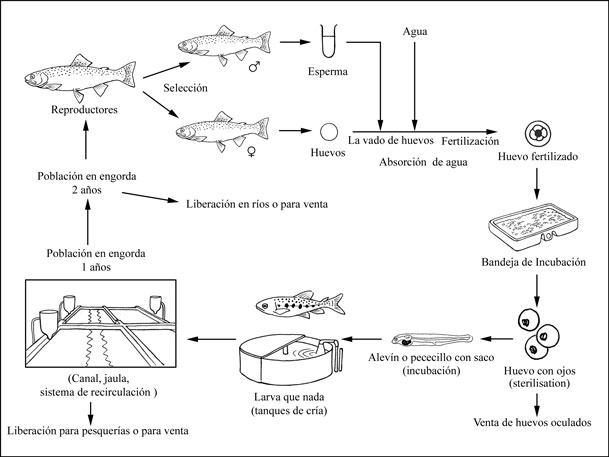
\includegraphics[width=15cm]{1} 
    \caption {Ciclo productivo de la trucha arcoiris}
    \label {fig:ciclo}
\end{figure}

Este pez es resistente, de crecimiento rápido y tolerante a una amplia
gama de manipulaciones y ambientes, pudiendo así ocupar una variedad de
hábitats y diferentes temperaturas. La temperatura ideal para el cultivo
de la trucha arcoiris está por debajo de 21º C, aunque en etapa de
desove y crecimiento la temperatura tiene que estar en el rango de 9 a
14ºC (Figura \ref{fig:ciclo}).

\subsection{Situación actual en Chile}

Los desembarques de Trucha arcoiris han aumentado cercano al 1500\% en
20 años (Figura \ref{desembarques}), con una tasa de crecimiento
porcentual promedio del alrededor del 15\% (Sernapesca, 2012), en
términos monetarios, el año 2013 la exportación de este producto generó
ventas alrededor de los 300 millones de dólares, lo que lo convierte en
una de las 3 especies más cosechadas en Chile junto al Chorito y el
Salmón del atlántico (Subpesca, 2013).

\begin{figure}[h]
    \centering
    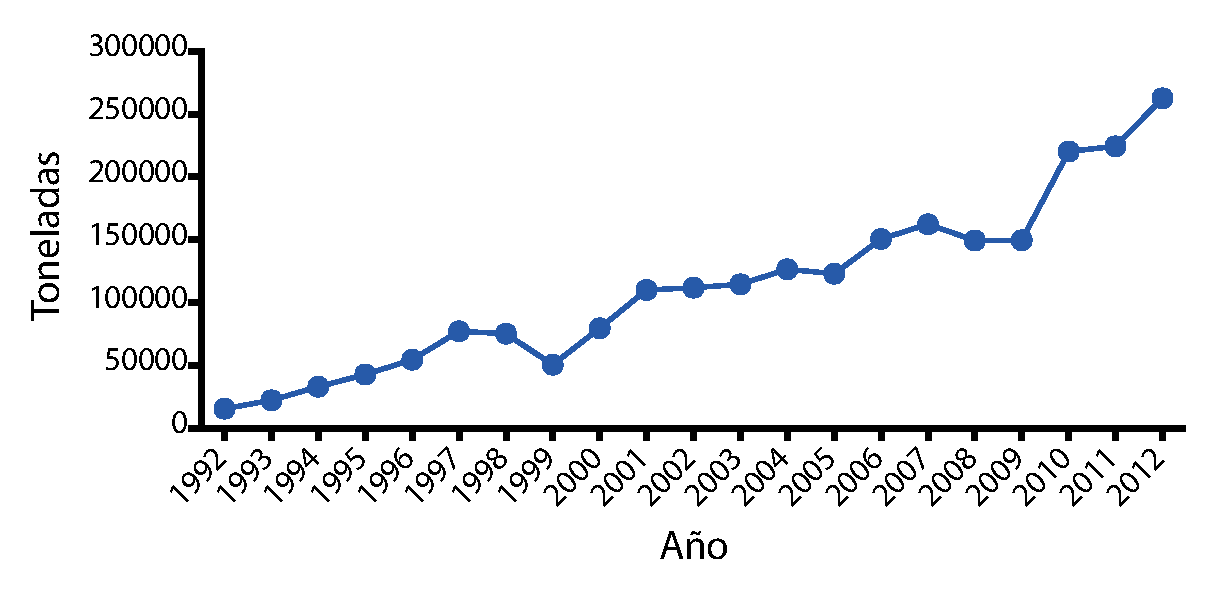
\includegraphics[width=0.9\textwidth]{desembarques.eps}
    \caption{Desembarques de Trucha arcoiris en Chile} \label{desembarques}
\end{figure}

Los sistemas de cultivo, debido al crecimiento acelerado de la
producción enfrentan diferentes problemas, por una parte patógenos como
\emph{Flavobacterium psychrophilum} y \emph{Piscirickettsia salmonis},
llegando a haber muertes en casos de hasta el 50\% y 34\% de la
producción respectivamente. La explicación de esto radica en la pérdida
del equilibrio ambiente-patógeno-hospedero, lo cual genera las
condiciones que hacen aumentar la enfermedad y mortalidad en el cultivo;
y por otra parte el estrés en que se ven sometidos los organismos
(Georgiadis et~al., 2001; FAO, 2012; Zwollo et~al., 2014). Estas
enfermedades, cualquiera sea su origen, pueden tener un alto impacto
negativo en la producción mundial, lo que equivale a grandes pérdidas
económicas (Shao, 2001). Para comprender y crear soluciones se requiere
conocer aspectos fundamentales de la defensa, especialmente del sistema
inmune.

\section{Sistema inmune en peces}

La comprensión de la funcionalidad del sistema inmune de peces,
especialmente en teleósteos, al igual que en vertebrados superiores se
puede entender como una respuesta innata o inespecífica y una respuesta
adaptativa o especifica (Olabuenaga, 2000; Fernández et~al., 2002). La
respuesta inmune innata o inespecífica en peces es muy importante, ya
que constituye la primera y más importante línea de defensa del pez
frente a un gran número de patógenos, en esta respuesta convergen
factores humorales y celulares ({Reyes Cerpa} et~al., 2012; Zhu et~al.,
2012). El sistema inmune tiene que ser efectivo en distinguir ``lo
propio'' de lo ``no propio'' y así poder combatir los patógenos (Athman
y Philpott, 2004). Los receptores de reconocimiento de patrones (PRR,
por sus siglas en inglés) de macrofagos, neutrofilos y células
dendríticas reconocen moléculas simples y patrones regulares de
estructuras moleculares conocidos como patrones moleculares asociados a
patógenos (PAMPs, por sus siglas en inglés), las cuales son moléculas
exógenas producidos solo por patógenos potenciales (Medzhitov y Janeway,
2000; Gordon, 2002; Kawai y Akira, 2010). Estos PRR reconocen
estructuras como oligosacáridos ricos en manosa, peptidoglicanos y
lipopolisacaridos en la pared celular bacteriana, así como también DNA
CpG no metilado, los que son comunes entre los patógenos y han sido
conservados durante la evolución (Roach et~al., 2005).

Los PRR tienen distintas funciones: estimular la ingestión y digestión
de los patógenos que reconocen, guiar las células al sitio de infección
e inducir la producción de moléculas efectoras, y se han encontrado
varios análogos de PRR de mamíferos en teleósteos y podemos encontrar
receptores de tipo Toll (TLR, por sus siglas en inglés), lectinas que
unen manosas (MBL, por sus siglas en inglés), receptores del
complemento, proteína C-reactiva, Dectina-1, entre otros
(Rondon-Barragan, 2010; Zhang et~al., 2014a). (Tabla \ref{tabla:prr})

\begin{table}[h!]
    \begin{center}
        \begin{threeparttable}
            \caption{Receptores de reconocimiento de patrones en Mamíferos y sus análogos en Teleósteos}\label{tabla:prr}
            \begin{tabularx}{\textwidth}{m{3cm} l X l}
                \toprule
                Familia & Taxón & Miembros & Referencia\\
                \midrule
                \multirow{8}{*}{\minitab[l]{TLRs}}                          &   Mamíferos               & TLR1, TLR2, TLR3, TLR4, TLR5, TLR6, TLR7, TLR8, TLR9, TLR10, TLR11, TLR12, TLR13          & \multirow{2}{*}{\minitab[l]{Jault et al., 2004 \\ Roach et al., 2005 \\ M. S. Lee y Kim, 2007}}       \\ \cline{2-3}
                                                                            &   Peces Teleósteos        & TLR1, TLR2, TLR3, TLR4, TLR5, sTLR5, TLR7, TLR8, TLR9, TLR14, TLR21, TLR22, TLR23         &                                       \\
                \midrule
                \multirow{3}{*}{\minitab[l]{Lectinas}}                      &   Mamíferos               & MBL, Intelectina, Pentraxinas, Dectina-1                                                  & \multirow{2}{*}{\minitab[l]{Russell y Lumsden, 2005 \\ M. S. Lee y Kim, 2007}} \\ \cline{2-3}
                                                                            &   Peces Teleósteos        & MBL, Intelectina, Pentraxinas                                                             &       \\
                \midrule
                \multirow{3}{*}{\minitab[l]{Receptores \\del complemento}}  &   Mamíferos               & CR3 y CR4 (Integrinas), C5aR                                                              & \multirow{2}{*}{\minitab[l]{Boshra et al., 2004 \\ M. S. Lee y Kim, 2007}} \\ \cline{2-3}
                                                                            &   Peces Teleósteos        & CD18 (Cadena $\beta$ de CR3 y CR4), C5aR                                                  & \\
                \midrule
                \multirow{3}{*}{\minitab[l]{NLRs}}                          & Mamíferos                 & NOD1, NOD2, NALPs, IPAF, NAIPS                                                            & \multirow{2}{*}{\minitab[l]{M. S. Lee y Kim, 2007 \\ Stein et al., 2007}} \\\cline{2-3}
                                                                            & Peces Teleósteos          & NOD1, NOD2                                                                                & \\
                \midrule
                \multirow{2}{*}{\minitab[l]{Helicasas CARD}}                & Mamíferos                 & RIG-1, MDA5                                                                               & \multirow{2}{*}{\minitab[l]{M. S. Lee y Kim, 2007 \\ M. Chang et al., 2011}} \\ \cline{2-3}
                                                                            & Peces Teleósteos          & RLR (RIG-1-Like receptor)                                                                 & \\
                \bottomrule
            \end{tabularx}
            \begin{tablenotes}
                \item 
            \end{tablenotes}
        \end{threeparttable}
    \end{center}
\end{table}

Entre los PAMPs más clásicos se puede encontrar a las secuencias de ADN
CpG sin metilar, los lipopolisacáridos (LPS) y el RNA bicatenario viral.
La interacción entre los PRR (como los TLR) y los PAMP es la reacción
que desencadenará e iniciará la transducción de señales intracelular que
resultara en la expresión de genes involucrados en la inflamación,
respuesta antiviral y maduración de células con fenotipo dendrítico
(Aghaallaei et~al., 2010); TLRs individuales activan factores de
transcripción únicos y comunes a través de diferentes vías de
señalización para generar una respuesta biológica especifica ante
microorganismos (Kawai y Akira, 2005; Boltaña et~al., 2011)

\begin{table}[h!]
    \begin{center}
        \begin{threeparttable}
            \caption{PAMPs y los patógenos que los producen}\label{tabla:pamps}
            \begin{tabularx}{0.7\textwidth}{l X}
                \toprule
                PAMP & Patógeno \\
                \midrule
                Lipopolisacárido (LPS)      & Bacteria gram-negativa                    \\
                \midrule
                Peptidoglicano              & \multirow{4}{*}{Bacteria gram-positiva}   \\
                Ácido Lipoteicóico          &                                           \\
                Lipopéptidos                &                                           \\
                Lipoarabinomanosa           &                                           \\
                \midrule
                Quitina                     & \multirow{2}{*}{Hongos y Levaduras}       \\
                Glucanos                    &                                           \\
                \midrule
                DNA CpG no-metilado         & Bacterias                                 \\
                \midrule
                DNA Doble y simple hebra    & Virus                                     \\
                \midrule
                Flagelina                   & Bacterias flageladas                      \\
                \bottomrule
                \end{tabularx}
                \begin{tablenotes}
                    \item
                \end{tablenotes}
                \end{threeparttable}    
                \end{center}
                \end{table}

Entre las células involucradas la fase celular inespecífica de la
respuesta inmune podemos encontrar las células citotóxicas no
específicas (NCC, por sus siglas en inglés), además se ha encontrado
evidencia que plantea la presencia de células tipo NK en peces, así
también como el reclutamiento de estas mediante células fagocíticas,
granulocitos y el factor NKEF (Athanasopoulou et~al., 2009; Bethke
et~al., 2012; Gomez et~al., 2013). Las células NCC en peces se
encuentran principalmente en el riñón cefálico, el bazo, sangre
periférica y el timo, son células citotóxicas inespecíficas, es decir
ejercen su acción en diferentes células diana sin un reconocimiento
previo, las cuales requieren un contacto célula-célula para poder
efectuar la lisis celular (Fischer et~al., 2013; Gomez et~al., 2013).
Dentro de las células fagocíticas los neutrófilos representan
aproximadamente en promedio a un 11\% de los leucocitos en sangre, son
también llamados polimorfonucleares o leucocitos específicos, su
capacidad fagocítica es baja, ya que ingieren poco material extraño,
aunque poseen la mayoría de la batería enzimática para este trabajo
(Palić et~al., 2011).

Dentro del sistema fagocítico mononuclear, podemos encontrar a los
monocitos y a los macrófagos, los primeros son móviles y generalmente
más grandes que los demás leucocitos, y en el caso de los macrófagos,
estos pueden fagocitar partículas mucho más grandes, y abundan en el
bazo y riñón cefálico, aunque también se han encontrado en tejido
linfoide asociado a mucosas (Olabuenaga, 2000; Castro et~al., 2011;
Gomez et~al., 2013).

\begin{figure}[h!]
    \centering
    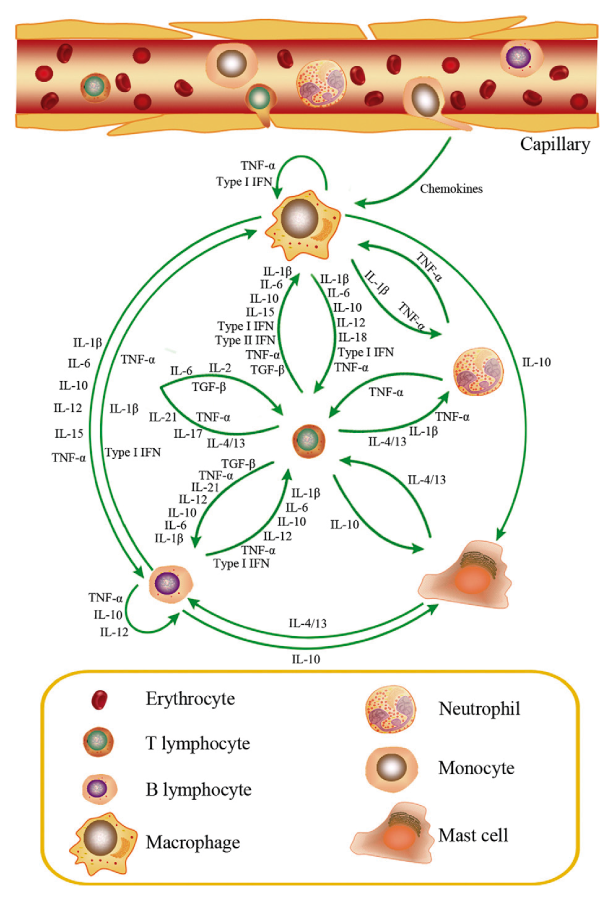
\includegraphics[width=10cm]{citoquinas} 
    \caption {Representación esquemática de las redes de citoquinas conocidas, involucradas en la regulación de funciones celulares en los peces, incluyendo la diferenciación, proliferación, supervivencia o apoptosis celular, y numerosas expresiones génicas. Tomada de Zhu et al., 2012}
    \label {fig:citoquinas}
\end{figure}

Entre los componentes moleculares asociados a la respuesta innata del
sistema inmune de peces se encuentran las citoquinas (Figura
\ref{fig:citoquinas}), moléculas de señalización celular particularmente
importantes en orquestar y regular la respuesta inmune. Son una familia
de proteínas de bajo peso molecular (comúnmente glicosiladas) y
secretadas por células del sistema inmune activadas previamente frente a
la exposición de diferentes componentes patógenos (Wang y Secombes,
2013). La respuesta inmune innata en mamíferos y peces está iniciada por
citoquinas de la familia de las interleuquinas (IL-1\(\beta\), IL-2,
IL-6), TNF-\(\alpha\) e IFN-\(\gamma\) (Uribe et~al., 2011), siendo
estas llamadas citoquinas pro-inflamatorias debido a a su rol en la
génesis de la respuesta inflamatoria (Savan y Sakai, 2006).

\begin{table}[h!]
    \begin{center}
        \begin{threeparttable}
            \caption{Interleuquinas de peces}\label{tabla:ils}
            \begin{tabular}{@{}lll@{}}
\toprule
Interleuquina & Organismo $^*$          & Referencia                \\ \midrule
IL-1$\beta$   & \textit{O.mykiss}   & Zou et al., 1999          \\
IL-18         & \textit{T.rubripes} & Huising et al., 2004      \\
IL-6          & \textit{T.rubripes} & Bird et al., 2005a        \\
IL-11         & \textit{O.mykiss}   & Wang et al., 2005         \\
IL-2          & \textit{T.rubripes} & Bird et al., 2005b        \\
IL-4          & \textit{T.rubripes} & Li et al., 2007           \\
IL-7          & \textit{T.rubripes} & Kono et al., 2008         \\
IL-15         & \textit{T.rubripes} & Bei et al., 2006          \\
IL-21         & \textit{T.rubripes} & Bird et al., 2005b        \\
IL-10         & \textit{T.rubripes} & Zou et al., 2003          \\
IL-22         & \textit{T.rubripes} & Zou et al., 2004          \\
IL-17         & \textit{D.rerio}    & Gunimaladevi et al., 2006 \\
IL-12         & \textit{T.rubripes} & Yoshiura et al., 2003     \\ \bottomrule
            \end{tabular}
                \begin{tablenotes}
                    \item $^*$ Se nombra el primer organismo donde fue reportada
                \end{tablenotes}
                \end{threeparttable}    
                \end{center}
                \end{table}

Las interleuquinas son citoquinas producidas principalmente por
linfocitos T CD4+, aunque también son secretadas por una gran variedad
de tipos celulares, como por ejemplo los macrófagos/monocitos y las
células endoteliales. En peces se ha descrito gran parte de las
interleuquinas presentes en mamiferos (Tabla \ref{tabla:ils}) (Secombes
et~al., 2011). Dentro de la familia de las interleuquinas podemos
encontrar la Interleuquina 1\(\beta\), la citoquina proinflamatoria mas
estudiada, todo debido a su rol mediador de enfermedades
autoinflamatorias. Es producida principalmente por macrófagos activados,
células dendríticas y monocitos, y afecta a casi cualquier tipo celular,
jugando un rol central en la generación de respuestas sistémicas y
locales a la infección, así como también en respuesta a daños y desafíos
inmunológicos (Reis et~al., 2012). Esta citoquina potencialmente induce
la proliferación, diferenciación y activación de células no específicas,
como NK y macrófagos, así como también una respuesta inmune específica,
activando linfocitos B y T (Hong et~al., 2004; Taechavasonyoo et~al.,
2013). Junto con IL-1\(\beta\) existe otro marcador que sirve para
evaluar si es que los inmunoestimulantes inducen o no una respuesta
inflamatoria, este otro marcador es el Factor de necrosis tumoral
(TNF-\(\alpha\)). este factor tiene una variedad de funciones
inmunológicas, regulando la inflamación y la respuesta inmune celular
(Zou et~al., 2003b; Wang et~al., 2004; Teles et~al., 2011). Promueve la
necrosis hemorrágica de tumores, así como también mejora la fagocitosis
y citotoxicidad de neutrófilos. Mejora la síntesis de prostaglandina E2
y oxido nítrico (NO), y modula la expresión de muchas citoquinas,
incluyendo IL-1, IL-6 y algunas quimioquinas. IL-1\(\beta\) y
TNF-\(\alpha\) son ampliamente usados como marcadores de respuesta
inmune innata (Zhang et~al., 2009). La interleuquina 12 (IL-12) es una
citoquina heterodimérica, compuesta por la subunidades P35 y P40, la
primera miembro de la familia de la interleuquina 6 con 4
\(\alpha\)-hélices en su topología y p40 recuerda una forma asociada a
un receptor de citoquinas solubles(Yoshiura et~al., 2003b; Huising
et~al., 2006). Esta citoquina pro-inflamatoria es producida en las
etapas iniciales de la respuesta inmune por monocitos, macrófagos,
celulas dendríticas y neutrófilos, y una de sus principales funciones es
inducir la síntesis de otras citoquinas, como IFN-\(\gamma\) (Zhang
et~al., 2014b).

Interferón Gamma (IFN-\(\gamma\)), perteneciente a la familia de los
Interferones de tipo II, importantes reguladores del sistema inmunitario
innato y adaptativo (Savan y Sakai, 2006). El IFN-\(\gamma\) es
producido en una primera etapa por celulas NK estimuladas por NKEF e
interleuquinas 12 y 18, las cuales son producidas por fagocitos
mononucleares y celulas presentadoras de antígenos (APCs, por sus siglas
en inglés). Al ser secretada esta molécula se une a su receptor y por la
via Jak/STAT promueve la activación de macrófagos aumentando la síntesis
de la fagocito oxidasa dependiente de NADPH (\si{gp91^{phox}} y
\si{p67^{phox}}), la oxido nítrico sintasa 2 (NOS2), p47 GTP-asa y la
proteína de unión a guanilato, así como también aumenta las moléculas de
MHC de clase 2 en macrófagos y otras APCs (Boehm et~al., 1997). Por lo
tanto en contraste con los interferones de tipo I
(IFN-\(\alpha\)/\(\beta\)) el IFN-\(\gamma\) juega un rol clave en la
activación de macrófagos para aumentar destrucción de patógenos
bacterianos, protozoos y virales (Fields et~al., 2007).

Dentro de las moléculas efectoras de la respuesta inmune la oxido
nítrico sintasa de tipo inducible (iNOS), propia de fagocitos (Wu
et~al., 2008; Zhao et~al., 2010), aumenta su expresión durante eventos
de inflamación, y a su vez, es propia del estallido respiratorio de los
macrófagos proveyendo así a la célula de un ambiente citotóxico ideal
para los eventos pro-inflamatorios por la producción de Oxido Nítrico
(NO), catalizando la oxídación de L-arginina (Yang et~al., 2013). Esta
molécula, puede ser activada en monocitos, macrófagos, células
dendríticas, neutrófilos y células NK ya sea por citoquinas,
endotoxinas, o ambas (MacMicking et~al., 1997; Bogdan, 2001). estas
características demuestran la importancia del rol de iNOS y su producto
gaseoso NO en el sistema inmune, haciendo de esta molécula un marcador
inmunológico de importancia para estudiar procesos inmunológicos.

Además de poseer una estructurada y bien desarrollada respuesta inmune
innata como se explicaba anteriormente, los peces también cuentan con
una respuesta adaptativa, con componentes celulares y humorales
(Alvarez-Pellitero, 2008), en este último grupo se encuentran los
anticuerpos, los cuales son proteínas pertenecientes al grupo de las
inmunoglobulinas (Ig), en el caso de los peces producen inmunoglobulinas
del tipo M, T y D (Bengtén et~al., 2002; Zhang et~al., 2011; Zhu et~al.,
2012), siendo la primera la más importante, estando presente en el
suero, el mucus y la bilis. Los anticuerpos son producidos por
linfocitos B activados al reconocer algún antígeno, ya sea en solución o
presentado por alguna célula presentadora de antígeno, que en el caso de
los peces principalmente son macrófagos, y tienen variadas funciones,
pueden actuar como moléculas efectoras en el suero, o también como
receptores de superficie de linfocitos B.

Una de las principales diferencias entre el sistema inmune de peces
teleósteos con el de mamíferos es la carencia de medula ósea y ganglios
linfáticos, por lo cual no se puede marcar una diferencia entre órganos
hematopoyéticos y órganos linfoides (Olabuenaga, 2000; Fernández et~al.,
2002). Entre los principales órganos pertenecientes al sistema inmune de
peces podemos encontrar el timo, el riñón y el bazo. El riñón cefálico
es el principal órgano en la diferenciación de linfocitos B, ya que es
el primer órgano en el que aparecen estas células durante el desarrollo
del pez, también es el órgano donde se produce la eritropoyesis,
granulopoyesis, linfopoyesis y monocitopoyesis (Whyte, 2007), por lo que
se le puede considerar a la vez un órgano análogo a la medula ósea de
los mamíferos (Razquin et~al., 1990). Los centros melanomacrofágicos son
una agregación de macrófagos que contienen melanina, un pigmento de
color oscuro, su tamaño y número está directamente relacionado con el
estado del pez, ya que estas variables aumentan considerablemente en
peces enfermos, donde el catabolismo ha sido excesivo. Algunos estudios
ontogénicos realizados en salmónidos sugieren que la función del bazo no
es esencial en la maduración del sistema inmunológico, ya que los
linfocitos del timo y riñón cefálico estarían más involucrados que este
órgano en esta maduración. Otros estudios sin embargo indican, que bajo
un desafío antigénico aparecen linfocitos B en el bazo, teniendo
parámetros similares a los presentados por estas células en otros
órganos como el riñón cefálico.

\section{Inmunidad de mucosas}

La mayoría de las infecciones empiezan o afectan las mucosas epiteliales
de los animales. El campo de la investigación en inmunología de mucosas
ha crecido sin precedentes durante los últimos años, así como también
nuestro conocimiento en la materia, específicamente como las superficies
de las mucosas responden a los variados antígenos que constantemente
invaden estos tejidos. En teleósteos los principales tejidos con
mucosas, y por ende las primeras barreras inmunológicas, son el
intestino, la piel y las branquias (Gomez et~al., 2013). El intestino,
la piel y las branquias contienen tejido linfoide asociado a mucosa
(MALT, por sus siglas en inglés) que tiene un rol fundamental en el
mantenimiento de la homeostasis en la mucosa. Este tejido linfoide
asociado a mucosa está dividido en tejidos linfoides asociados a
intestino, piel y branquias (GALT, SALT y GIALT, respectivamente, por
sus siglas en inglés). Estas superficies mucosas están cubiertas por una
capa protectora de mucus rico en factores inmunológicos, como las
lectinas, mucinas, peptidos antimicrobianos, toxinas e inmunoglobulinas
(Lazado y Caipang, 2014).

\begin{figure}[h!]
    \centering
    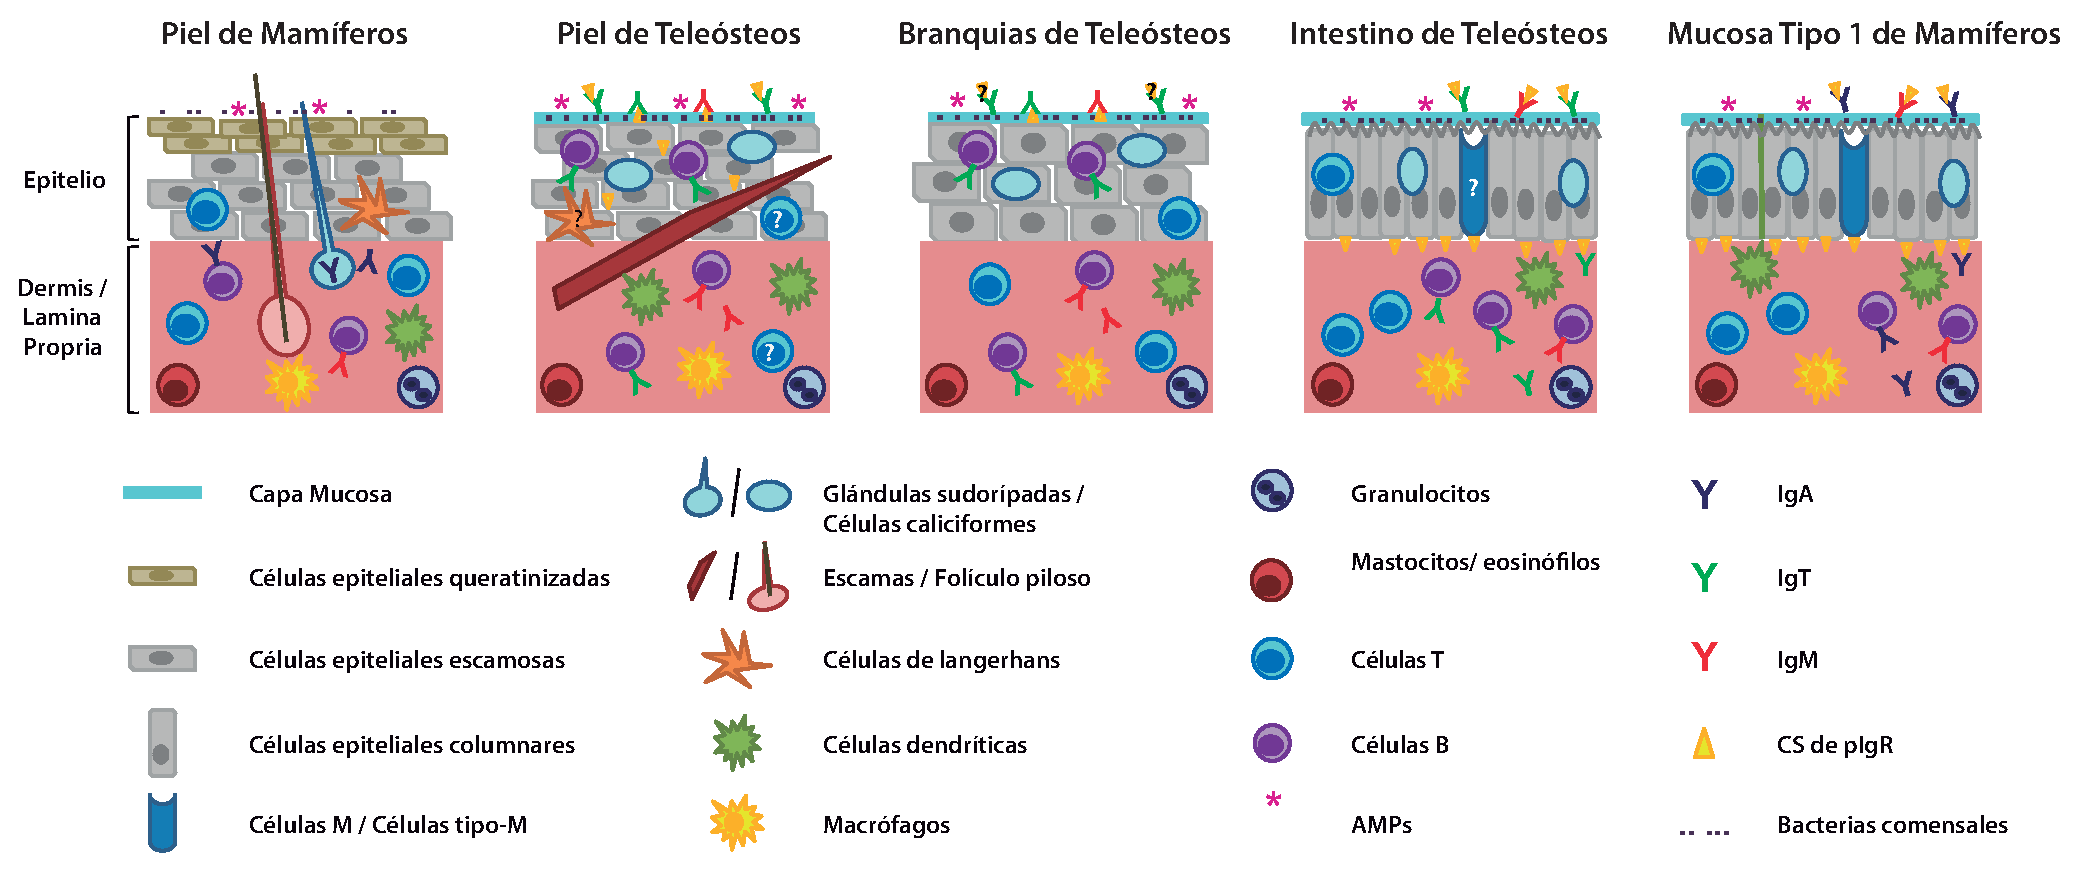
\includegraphics[width=\textwidth]{mucosalimmunity} 
    \caption {Representación esquemática de las similitudes y diferencias entre las superficies mucosas de teleósteos como piel, intestino y branquias y de mamiferos como piel y mucosa de tipo 1. Adaptado y traducido desde Gomez et al., 2013}
    \label {fig:mucosal}
\end{figure}

Las principales diferencias estructurales y funcionales entre las
superficies mucosas de mamíferos tipo 1 con las de teléosteos son la
falta de tejido linfoide organizado como los placas de Peyer, así como
también células M como tal o la inmunoglobulina A secretada
(\(\mathrm{_{sec}}\)IgA, por sus siglas en inglés) todavía no han sido
descritas en peces (Rombout et~al., 2011). A pesar de estas diferencias
los intestinos, piel y branquias de los peces comparten muchas
características con las superficies mucosas de tipo 1 en mamíferos (Fig.
\ref{fig:mucosal}).

\subsection{Inmunidad Branquial}

Las branquias de los peces son, en términos de superficie expuesta, el
mayor tejido en muchas especies de teleósteos (1m\textsuperscript{2}/kg
en carpa), siendo el órgano principal para mantener la homeostasis del
pez por la ingesta de nutrientes y sustancias, así como también formando
una barrera activa en contra de la entrada de patógenos (Oikawa y
Itazawa, 1985). Morfológicamente, las branquias consisten en una
laminilla, la cual comprende la principal superficie respiratoria del
pez (Wilson y Laurent, 2002). El epitelio presente en las branquias
contiene una a cuatro capas cúbicas o escamosas de células, a su vez
también presenta células caliciformes, encargadas de la producción de
mucus. La ubicación morfológica de las branquias le confieren un lugar
expuesto al ambiente acuático, por lo que es un sitio esencial para que
bacterias y otros patógenos entren al organismo del pez, siendo un sitio
con una sustancial exposición a distintos tipos de antígenos. El GIALT
cuenta con macrófagos y granulocitos (Mulero et~al., 2008), componentes
de la respuesta adaptativa como células B y T (Scapigliati et~al., 1999;
Santos et~al., 2001; Salinas et~al., 2011), así como también e una alta
expresión de los genes relacionados con células T (Boschi et~al., 2011).

\section{Inmunomoduladores}

Los inmunomoduladores han sido descritos como componentes necesarios
para la acuicultura, ya que mejoran la respuesta innata y proveen
resistencia frente a diferentes patógenos. Estas sustancias, como los
\(\beta\)-glucanos, productos bacterianos y constituyentes de las
plantas pueden iniciar directamente la activación de mecanismos de
defensa innata actuando en receptores y desencadenando la activación de
distintos genes que puedan resultar en la producción de moléculas
antimicrobianas (Bricknell y Dalmo, 2005; Kumari y Sahoo, 2006). A pesar
de la evidencia demostrada sobre el uso benéfico de estas sustancias
como potenciales inmunomoduladores de la respuesta frente a distintos
patógenos en la acuicultura (Bricknell y Dalmo, 2005; Dalmo y Bøgwald,
2008; Bilen et~al., 2011; Abarca et~al., 2012; Chettri et~al., 2013),
las actuales soluciones comerciales están de cierta manera restringidas
por ser derivadas de algunas levaduras, como por ejemplo los \(\beta\)
1-3, \(\beta\) 1-6 glucanos que son vendidos bajo la marca MacroGard® y
sus distintos derivados. Existe también un producto comercial llamado
Ergosan, el cual está hecho de una mezcla de distintos componentes de un
alga, la cual es rica en alginatos y polisacáridos. Una dosis individual
de 1mg de Ergosan aumenta significativamente la proporción de
neutrófilos, aumentan el grado de fagocitosis, la actividad del
estallido respiratorio y la expresión de interleuquina 1\(\beta\)
(IL-1\(\beta\)), interleuquina 8 (IL-8) y el factor de necrosis tumoral
alfa (TNF-\(\alpha\)) en leucocitos peritoneales de trucha arcoíris a 1
dia post inyección (Peddie et~al., 2002).

\subsection{$\beta$-glucanos}

\begin{table}[h!]
    \sffamily
    \begin{center}
        \begin{threeparttable}
            \captionsetup{font={normalsize,sf}}
            \caption{Estructuras de $\beta$-Glucanos según su origen}\label{tablaglucanos}
            \begin{tabularx}{13cm}{l c X}
                \toprule
                Origen & Estructura & Función \\
                \midrule
                Bacteriano & 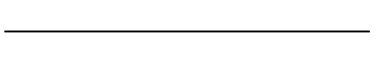
\includegraphics[width=3cm]{bgbacteriano} & $\beta$1,3-Glucano lineal con ramificaciones largas de $\beta$1,6-Glucano\\
                Levadura & 
\includegraphics[width=3cm]{bglevadura} & $\beta$1,3-Glucano Lineal \\ 
                Cereal & 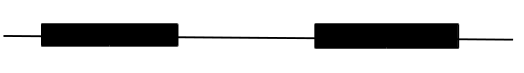
\includegraphics[width=3cm]{bgcereal} & $\beta$1,3/$\beta$1,4-Glucano lineal \\
                Hongo & 
\includegraphics[width=3cm]{bghongo} & $\beta$1,3-Glucano lineal con ramificaciones cortas de $\beta$1,6Glucano \\
                \bottomrule
            \end{tabularx}
            \begin{tablenotes}
                \item Estructuras de $\beta$-Glucanos según su origen
            \end{tablenotes}
        \end{threeparttable}
    \end{center}
\end{table}

Los \(\beta\)-glucanos son carbohidratos que consisten en moléculas de
glucosas enlazadas, los cuales son componentes estructurales de gran
importancia en paredes celulares de levaduras, hongos, algas y algunas
bacterias. Estos carbohidratos también forman parte de la pared celular
endospermas de algunos cereales como la cebada y la avena. Dependiendo
del origen del \(\beta\)-glucano encontraremos diferencias también en
sus estructuras moleculares y sus posibles ramificaciones (Tabla
\ref{tablaglucanos}) (Volman et~al., 2008; Skov et~al., 2012).

\begin{table}[h!]
    \renewcommand{\arraystretch}{0.8}% Tighter
    \begin{center}
        \begin{threeparttable}
            \caption{Efectos inmunomoduladores de $\beta$-glucanos en peces}\label{tabla:glucanos}
            \begin{tabularx}{\textwidth}{l l l X l}
                \toprule
                $\beta$-Glucano & Entrega & Especie & Efecto & Referencia\\
                \midrule
                Macrogard                       &   Oral                & \emph{C.carpio}               & $\uparrow$ CRP $\uparrow$ C3                  & Pionnier \emph{et al}., 2014          \\
                & & & & \\
                Macrogard                       &   IIP                 & \emph{D.labrax}               & $\uparrow$ HSP $\uparrow$ Lisozima                    & Bagni et al., 2005            \\
                                                &                       &                               & $\uparrow$ Complemento            &                       \\
                & & & & \\
                Laminarán                       &   IIP                 & \emph{O.mykiss}               & $\uparrow$ IL-1$\beta$ $\uparrow$ IL-6            & Løvoll et al., 2007       \\
                                                &                       &                               & $\uparrow$ C3-1   $\uparrow$ C3-2 $\uparrow$ C3-3         &                       \\
                & & & & \\
                Paramylon                       &   Baño                & \emph{O.mykiss}               & $\uparrow$ Hepcidina  $\uparrow$ Factor B             & Chettri et al., 2013      \\  
                                                &                       &                               & $\uparrow$ Preceberelina $\uparrow$ C3            &                       \\
                & & & & \\
                $\beta$1,3-Glucano              &   Baño, IIP           & \emph{C.carpio}               & $\uparrow$ Leucocitos Sanguíneos  & Selvaraj et al., 2005         \\
                \emph{S. cerevisiae}            &   Oral                &                               & $\downarrow$ Mortalidad $\uparrow$ IL-1$\beta$ mRNA           &                       \\
                                                &                       &                               & $\uparrow$ Producción anticuerpos &                       \\                                              
                & & & & \\
                Laminarán                       &   Oral, IIP           & \emph{O.mykiss}               & $\uparrow$ TNF-$\alpha$ $\uparrow$ IL-8           & Morales-Lange et al., 2014    \\
                                                &                       &                               & $\uparrow$ AF $\uparrow$ CF                   &                       \\
                & & & & \\
                $\beta$1,3-Glucano              &   Oral                & \emph{L.crocea}               & $\downarrow$ Mortalidad $\uparrow$ AF             & Ai et al., 2007               \\
                \emph{S.cerevisiae}             &                       &                               & $\uparrow$ Estallido Respiratorio                     &                       \\
                & & & & \\
                $\beta$-D-Glucano               &   IIP                 & \emph{L.rohita}               & $\downarrow$ Mortalidad           & Misra et al., 2006            \\
                Cebada                          &                       &                               & $\uparrow$ Lisozima $\uparrow$ AF $\uparrow$ AB               &                       \\
                & & & & \\
                Macrogard                       &   Oral                & \emph{C.carpio}               & $\uparrow$ Gen MX $\uparrow$ TLR3,1               & Falco et al., 2014            \\
                                                &                       &                               & $\uparrow$ IL-1$\beta$ $\uparrow$ TNF-$\alpha$            &                       \\
                & & & & \\
                $\beta$1,3-Glucano              &   Baño                & \emph{O.mykiss}               & $\uparrow$ IFN-$\gamma$ $\uparrow$ TNF-$\alpha$           & Skov et al., 2012             \\
                \emph{E.gracilis}               &                       &                               & $\uparrow$ Hepcidina          &                       \\
                \bottomrule
            \end{tabularx}
            \begin{tablenotes}
                \item IIP: Inyección intra-peritoneal, AF: Actividad Fagocítica, CF: Capacidad Fagocítica \\
            \end{tablenotes}
        \end{threeparttable}
    \end{center}
\end{table}

\(\beta\)-glucanos derivados de diferentes especies pueden variar en su
estructura y su bioactividad (Akramiene et~al., 2007). Las diferencias
como el largo de su cadena de polisacáridos, la presencia o no de
ramificaciones, y el largo de esas ramificaciones pueden influenciar
finalmente en el método de extracción, los componentes insolubles e
incluso en los pesos moleculares (Akramiene et~al., 2007). Diferencias
como el método de extracción o su solubilidad pueden afectar la
bioactividad de estos componentes, sobretodo teniendo en cuenta que
existen estudios que han demostrado que el \(\beta\)-(1,3/1,6)-glucano
tiene mejor actividad biológica que su forma soluble
(\(\beta\)-(1,3/1,6)-glucano) (Ooi y Liu, 2000).

En peces ha sido estudiado el uso de \(\beta\)-glucanos como
inmunoestimulantes, en distintas especies, como en ciprínidos
(\emph{C.koi, C.carpio}) (Lin et~al., 2011; Kühlwein et~al., 2014),
salmónidos (Abarca, 2011; Skov et~al., 2012), pez cebra
(\emph{Danio rerio}) (Rodríguez et~al., 2009), entre otros (Wang et~al.,
2007; Lokesh et~al., 2012), demostrando que estos inmunomoduladores
pueden estimular la actividad fagocítica de macrófagos, promoviendo la
producción de proteínas líticas como la lisozima y el complemento,
generando un \emph{boost} en la respuesta innata del pez.

En mamíferos el principal receptor de \(\beta\)-glucanos pertenece la
familia de las Lectinas de tipo C y es llamado Dectina-1 (Brown y
Gordon, 2001). En peces existe muy poca información relevante a los
receptores específicos para \(\beta\)-glucanos. En macrófagos de
\emph{Salmo salar} estimulados con un \(\beta\)-1,3-glucano de levaduras
sugieren la presencia de un receptor específico que podría reconocer
cadenas de \(\beta\)-glucanos (Engstad y Robertsen, 1994). Finalmente,
un estudio realizado en 2013, usando Zimosán y agonistas específicos
para los receptores Dectina-1 demostraron que los macrófagos de la carpa
son poco, pero no insensibles a los agonistas selectivos de Dectina-1,
sugiriendo que el reconocimiento de \(\beta\)-glucanos puede ser
efectuado por múltiples PRR, incluyendo receptores TLR y no-TLR
(Pietretti et~al., 2013).

Existen evidencias a nivel de GIALT de respuesta inmune sistémica
(Bethke et~al., 2012) y además se ha demostrado que el consumo en dieta
o la suplementación por inyección de \(\beta\)-glucanos modifica la
disponibilidad de TNF-\(\alpha\) e IL-8 en trucha arcoíris
(Morales-Lange et~al., 2014).

La inmunoestimulación oral afecta distintos parámetros inmunológicos, y
a su vez existen antecedentes de estos cambios a nivel de mucosas como
la piel, los intestinos y las branquias.

No obstante no existe un modelo molecular que indique el espectro de
moléculas reguladoras y efectoras de inmunidad a evaluar, ni existe un
consenso con los tiempos asociados a la expresión y disponibilidad de
éstas. Teniendo en cuenta que los estudios disponibles a la fecha solo
usan una aproximación a nivel de transcrito, habiendo pocos estudios
sobre disponibilidad de proteínas, es necesario que la evaluación de
estos parámetros relacione su nivel de transcripción con la
disponibilidad de proteínas, para saber qué, cuándo y con qué método
evaluar al momento de suplementar la alimentación de estos organismos
con \(\beta\)-glucanos como inmunomoduladores.

Se requiere un analisis que correlacione la cuantificación de ambos
parametros para establecer cual es el mejor indicador molecular del
efecto inmunomodulador de \(\beta\)-glucanos.

\chapter{Hipótesis}

La inmunomodulación en tejido branquial de \emph{O.mykiss} generada por
la liberación en dieta del \(\beta\)-glucano \emph{Zimosán A} es
cuantificable, lo que permite establecer un modelo y relacionar los
niveles de la expresión y disponibilidad de moléculas reguladoras y
efectoras de la inmunidad. \chapter{Objetivo General}

Establecer un modelo molecular basado en la magnitud de la expresión y
disponibilidad de diferentes parámetros de respuesta inmunológica en
tejido branquial de \emph{O.mykiss} en respuesta a la liberación en
dieta del \(\beta\)-glucano Zymosan A.

\section{Objetivos Específicos}

\begin{enumerate}
\def\labelenumi{\arabic{enumi}.}
\itemsep1pt\parskip0pt\parsep0pt
\item
  Implementar un sistema de alimentación para la liberación en dieta de
  Zimosán A y sus respectivos controles de \emph{O.mykiss}
\item
  Evaluar la expresión de moléculas efectoras y reguladoras de respuesta
  inmune en tejido branquial de \emph{O.mykiss} tratados con Zimosán A
  liberado en dieta.
\item
  Detectar la disponibilidad de proteínas efectoras y reguladoras de
  respuesta inmune en tejido branquial de \emph{O.mykiss} tratados con
  Zimosán A liberado en dieta.
\item
  Correlacionar el nivel de expresión y detección de moléculas de
  respuesta inmune evaluadas en tejido branquial.
\end{enumerate}

\clearpage

\chapter{Materiales y Métodos}

\begin{figure}[h!]
    \centering
    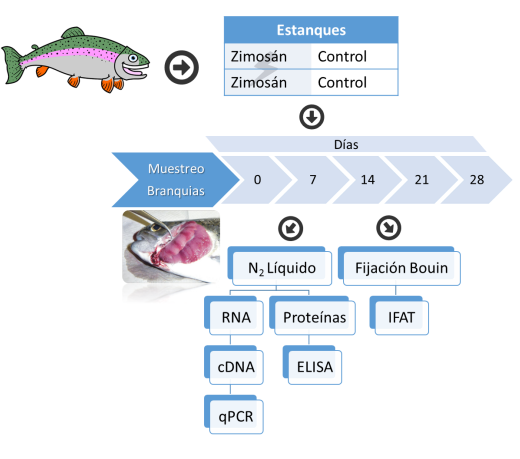
\includegraphics[width=9cm]{esquema} 
    \caption {Esquema general de trabajo}
    \label {fig:esquema}
\end{figure}

\section{Material Biológico y Bioensayo}\subsection{Peces}

Ejemplares de truchas arcoiris con un peso promedio de 22,26 \(\pm\)
1,7397g fueron obtenidas desde la piscicultura de Rio Blanco, ubicada a
35km de Los Andes, en la Quinta región de Valparaíso y fueron
trasladados hasta el Centro de Investigaciones en Acuicultura Curauma
(CIAC), ubicado en la provincia de Valparaíso. Fueron aclimatados
durante 1 semana y se mantuvieron a 14º C durante toda la investigación.

\subsection{Dieta}

La dieta base de las truchas consistió en un pellet que contenía 65\% de
harina de pescado, 16,3\% harina de trigo, 16\% aceite de pescado, 0.1\%
vitamina C, 1\% Premix Vitamínico, 1\% Premix minerales traza, 0.6\%
Colina + Gluten de Maiz

\subsection{Parametros fisicoquimicos del ensayo}

Durante toda la experiencia se midió dia a dia la temperatura, pH,
presión y saturación de oxigeno de cada estanque y modulo llenando una
planilla dispuesta para ese fin por el CIAC.

\subsection{Anticuerpos}

Se utilizarán anticuerpos policlonales monoespecíficos, obtenidos en
ratones y conejos, inmunizados con epítopes sintéticos de las moléculas
de interés. Estas moléculas han sido validadas en salmónidos, mediante
técnicas estandarizadas en el Grupo de Marcadores Inmunológicos del
Laboratorio de Genética e Inmunología Molecular de la Pontificia
Universidad Católica de Valparaíso (GIM-PUCV) (Narváez et~al., 2010;
Bethke et~al., 2012; Rojas et~al., 2012; Santana et~al., 2012)

\begin{table}[h!]
    \sffamily
    \begin{center}
        \begin{threeparttable}
        \caption{Lista de Anticuerpos Usados}\label{tabla:anticuerpos}
            \begin{tabularx}{16cm}{l l l X l l l}
                \toprule
                \multicolumn{4}{c}{} & \multicolumn{3}{c}{Dilución Anticuerpo} \\
                \cmidrule(r){5-7}
                Molécula (Anti) & Huesped & Origen & Secuencia epítope & ELISA & WB & IFAT \\
                \midrule
                TNF-$\alpha$ & Conejo & Suero & \texttt{WRKDDGQAFSQGGFE} & 1:2000 & 1:500 & 1:500 \\
                TNF-$\alpha$ & Ratón & Suero & \texttt{ } & - & 1:500 & - \\
                IL-1$\beta$ & Conejo & Suero &  \texttt{DLLNFLLESAVEEHI} & 1:2000 & 1:500 & 1:500 \\
                IL-1$\beta$ & Ratón & L.A. & \texttt{} & - & 1:250 & - \\
                IFN-$\gamma$ & Conejo & Suero & \texttt{ASKLALKIHLKKDN} & 1:2000 & 1:500 & 1:500 \\
                IFN-$\gamma$ & Ratón & Suero & \texttt{ } & - & 1:500 & - \\
                iNOS & Ratón & Suero & \texttt{CFIYSSGGFHLPAEPSTPVI} & 1:1000 & 1:500 & 1:250 \\
                IL-12 & Ratón & L.A. & \texttt{TETQVPLLCGDSYQDTE} & 1:1000 & 1:500 & 1:250 \\
                \bottomrule
            \end{tabularx}
            \begin{tablenotes}
                \item *L.A. = Líquido Ascítico, WB = Western Blot, IFAT = \emph{Immunofluorescence Antibody Test}
            \end{tablenotes}
        \end{threeparttable}
    \end{center}
\end{table}

\begin{table}[h!]
    \begin{center}
        \begin{threeparttable}
            \caption{Lista de Anticuerpos Comerciales Usados}\label{tabla:anticuerpos-comerciales}
                \begin{tabular}{l l l l l}
                \toprule
                Reactividad & Huesped & Conjugado & Dilución & Proveedor \\
                \midrule
                IgG (H+L) Ratón & Cabra & HRP & 1:7000 & Thermo Pierce (31430) \\
                IgG (H+L) Conejo & Cabra & HRP & 1:5000 & Thermo Pierce (31460) \\
                IgG (H+L) Ratón & Cabra & Alexa Fluor 568 & 1:400 & Life Technologies (A-11004) \\
                IgG (H+L) Conejo & Cabra & Alexa Fluor 488 & 1:400 & Life Technologies (A-31576) \\
                \bottomrule
                \end{tabular}
            \begin{tablenotes}
                \item *HRP = \emph{Horse radish peroxidase}
            \end{tablenotes}
        \end{threeparttable}
    \end{center}
\end{table}

\section{Desafío y Controles}

Los especímenes de trucha arcoíris se alimentaran en dos grupos,
inducidos y controles, el primer grupo tendrá una dieta al 3\% de su
peso con un agregado del 0,3\% de Zimosán, los controles tendrán la
misma alimentación excepto por el Zimosán, el cual será reemplazado con
PBS.

\section{Muestreo}

Los peces se sacrificaron con sobredosis del sedante Kalmagin 20\%
(Benzocaína 20\% CentroVet), se pesaron los peces y luego tomaron
muestras los días 0, 7, 14, 21 y 28, 5 peces por condición, intercalando
3 peces de un estanque y 2 de su par respectivo en cada día de muestreo
(Tabla \ref{tablaidentificantes}). Las muestras se tomaron en dos
grupos, primero se tomaron ejemplares de branquias y se fijaron con
solución de Bouin (71\% solución saturada al 1,2\% de Ácido pícrico,
24\% formaldehído y 5\% ácido acético glacial) por 7 horas y luego se
lavaron 3 veces con Etanol al 70\% , dejándolos en este alcohol hasta su
posterior uso. Para el otro grupo se procedió a pulverizar con Nitrógeno
Líquido usando un mortero, para ser usado en las extracciones de RNA y
Proteínas.

\begin{table}[h!]
    \begin{center}
        \begin{threeparttable}
            \caption{Identificantes de muestras}\label{tablaidentificantes}
            \begin{tabular}{l l l l l l l l l l}
                \toprule
                ID & Muestra & ID & Muestra & ID & Muestra & ID & Muestra & ID & Muestra\\
                \midrule
                B1 & d0B1 & B21 & d7Bz3 & B31 & d14Bz3 & B41 & d21Bz3 & B51 & d28Bz3 \\
                B2 & d0B2 & B22 & d7Bz3 & B32 & d14Bz3 & B42 & d21Bz3 & B52 & d28Bz3 \\
                B3 & d0B3 & B23 & d7Bz3 & B33 & d14Bz4 & B43 & d21Bz3 & B53 & d28Bz4 \\
                B4 & d0B4 & B24 & d7Bz4 & B34 & d14Bz4 & B44 & d21Bz4 & B54 & d28Bz4 \\
                B5 & d0B5 & B25 & d7Bz4 & B35 & d14Bz4 & B45 & d21Bz4 & B55 & d28Bz4 \\
                B16 & d7Bc1 & B26 & d14Bc1 & B36 & d21Bc1 & B46 & d28Bc1 & \\
                B17 & d7Bc1 & B27 & d14Bc1 & B37 & d21Bc1 & B47 & d28Bc1 & \\
                B18 & d7Bc1 & B28 & d14Bc2 & B38 & d21Bc1 & B48 & d28Bc2 & \\
                B19 & d7Bc2 & B29 & d14Bc2 & B39 & d21Bc2 & B49 & d28Bc2 & \\
                B20 & d7Bc2 & B30 & d14Bc2 & B40 & d21Bc2 & B50 & d28Bc2 & \\
                \bottomrule
            \end{tabular}
            \begin{tablenotes}
                \item   d = Día Muestreo (0,7,14,21,28); B = Branquia; \\
                        c = Estanques control (1,2); z = Estanques inducidos (3,4)
            \end{tablenotes}
        \end{threeparttable}
    \end{center}
\end{table}

\clearpage

\section{Extracción de RNA}\label{extraccionrna}

La extracción de RNA se llevó acabo usando el Kit de OmegaBiotek E.Z.N.A
Total RNA Kit II usando las instrucciones del fabricante, para el
homogenizado adicional se usó el homogenizador de sobremesa FastPrep24
de MP Biomedicals con un programa de 4,5 movimientos por segundo durante
40 segundos usando como matriz 4 esferas metálicas de 2,388mm de
diametro.

\subsection{Cuantificación e Integridad de RNA}

El RNA se cuantificó usando el sistema espectrofotométrico ND-1000 de
NanoDrop cargando 2\si{\micro\liter} del RNA previamente extraído, luego
para verificar su integridad se corrió un gel de agarosa nativo al 0,8\%
durante 1 hora a 80V cargando 1\si{\micro\gram} de RNA por pocillo, el
RNA se almacenó a -80ºC.

\subsection{Sintesis de cDNA}

La transcripción reversa para generar el DNA complementario al RNA
previamente extraido se realizó usando el Kit M-MLV Reverse
Transcriptase de Promega usando las instrucciones del fabricante con
1\si{\micro\gram} de RNA, la reacción se hizo en un Termociclador C1000
Touch de Bio-Rad.

Para asegurar que las amplificaciones eran obtenidas a partir del cDNA y
no de restos de DNA genómico no eliminado por el tratamiento con DNAsa
I, previo a las reacciones de retrotranscripción, se realizaron
reacciones de PCR control en las que como molde se utilizaron los RNAs
extraídos. El tratamiento con DNAsa I se repetía, si era necesario,
hasta que en todos los casos se obtenía una amplificación nula, de
manera que el RNA molde para las reacciones de retrotranscripción
estuviese totalmente libre de DNA genómico.

\section{PCR en Tiempo Real (qPCR)}

La cuantificación por PCR a tiempo real permite monitorizar la reacción
de PCR al mismo tiempo que ésta tiene lugar. Se empleó como estrategia
para realizar la cuantificación el uso de la sonda SYBR Green® del kit
Brilliant III Ultra-Fast (Agillent) (Wittwer et~al., 1997). Las
reacciones de PCR se llevaron a cabo en un termociclador a tiempo real
CFX96 (Bio-Rad). Esta mezcla incluye, en las cantidades adecuadas y
listo para su uso, la enzima ``\emph{Taq} DNA Polimerasa'', dNTPs, MgCl2
y el tampón de PCR, e incorpora, como su nombre indica, el colorante
SYBR Green I, que detecta DNA de doble hélice, por lo que no es
necesario el uso de sondas específicas. Las muestras se amplificaron por
duplicado en placas de 96 pocillos para reacciones ópticas (Hard-Shell
de Bio-Rad) (Figura \ref{fig:placapcr}).

\begin{figure}[h!]
    \centering
    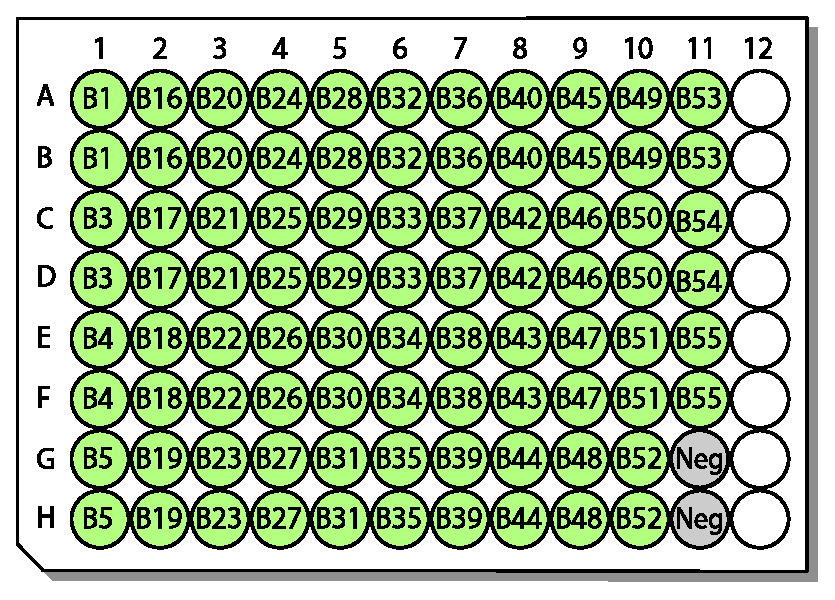
\includegraphics[width=8cm]{placaqpcr}
    \caption {Diseño de placa para PCR en tiempo real}
    \label {fig:placapcr}
\end{figure}

\subsection{Estandarización de partidores}

\begin{table}[h!]
    \begin{center}
        \begin{threeparttable}
            \caption{Lista de Partidores}\label{tabla:partidores}
            \begin{tabularx}{15cm}{l l X r}
                \toprule
                \textbf{Molécula}   & \textbf{Partidor} & \textbf{Secuencia} & \textbf{Amplicón} \\
                \midrule
                EF-1$\alpha$        & Fw    & \texttt{TGG AGA CTG GCA CCC TGA AG}       & 127 pb    \\
                                    & Rev   & \texttt{CCA ACA TTG TCA CCA GGC ATG G}    &           \\
                IL-1$\beta$         & Fw    & \texttt{GTC ACA TTG CCA ACC TCA TCA TCG}  & 95 pb     \\
                                    & Rev   & \texttt{GTT GAG CAG GTC CTT GTC CTT GA}   &           \\
                TNF-$\alpha$        & Fw    & \texttt{GTG TGG GGT CCT CTT AAT AGC AGG}  & 88 pb     \\
                                    & Rev   & \texttt{CTG CAT CGT TGA CGG TCT TCC}      &           \\
                IFN-$\gamma$        & Fw    & \texttt{GCT GTT CAA CGG AAA ACC TGT TT}   & 51 pb     \\
                                    & Rev   & \texttt{TCA CTG TCC TCA AAC GTG}          &           \\
                iNOS                & Fw    & \texttt{TAT GCT CTG CCT GCC GTG TC}       & 158 pb    \\
                                    & Rev   & \texttt{ATC CTG CGA CCC ACT TCC TC}       &           \\
                IL-12               & Fw    & \texttt{TTT AAT CAG CTG TCG GGC CAA GTC}  & 123 pb    \\
                                    & Rev   & \texttt{GTG CAA GAT TCC TGG CTG TCA GTA}  &           \\
                \bottomrule                         
            \end{tabularx}
            \begin{tablenotes}[normal,flushleft,rm]
                \item Tabla de partidores usados para la amplificación de las moléculas en estudio, se indica el tamaño esperado en pares de bases del amplicón. \\ Fw = Forward, Rev= Reverse, pb = Pares de Bases
            \end{tablenotes}
        \end{threeparttable}
    \end{center}
\end{table}

Usando un mix de varios cDNA al azar (controles e inducidos) se
estandarizaron los distintos partidores usados en el ensayo, usando
diluciones en agua DEPC 1:1 1:2 1:4 1:8 de este mix en cada placa (1µL
en total), por cada partidor, luego el software CFX Manager (Bio-Rad)
entregó las informaciones necesarias para determinar el uso o no de un
partidor en base a un programa del termociclador y un gradiente de
temperaturas (Tabla \ref{tabla:estandar}).

\begin{table}[h!]
    \begin{center}
        \begin{threeparttable}
            \caption{Programa Termociclador para estandarización de Partidores}\label{tabla:estandar}
            \begin{tabularx}{13cm}{l X l l}
                \toprule
                Etapa & Temperatura & Tiempo & Ciclos \\
                \midrule
                Denaturación Inicial & 95º & 03:00 min & 1 \\
                Denaturación & 95º & 00:10 seg & 39\\
                Annealing en Gradiente & 62º $\rightarrow$ 52* & 00:10 seg & 39 \\
                Extensión & 60º & 00:10 seg & 39 \\
                \bottomrule
            \end{tabularx}
            \begin{tablenotes}
                \item El gradiente varía dentro de esas temperaturas según los partidores
            \end{tablenotes}
        \end{threeparttable}
    \end{center}
\end{table}

\subsection{Master Mix para cada reacción}

Cada reacción se llevó a cabo en un volumen de 10µl según la Tabla
\ref{mmix}. Las condiciones térmicas de la amplificación fueron las
siguientes: un ciclo inicial de 3 minutos a 95ºC (activación
enzimática), seguido por 39 ciclos de 5 segundos a 95ºC, 5 segundos a
58º para todos los partidores exceptuando los partidores para
IFN-\(\gamma\) que fue de 61,5º y 15 segundos a 72ºC (desnaturalización,
\emph{annealing} y extensión respectivamente).

\begin{table}[h!]
    \begin{center}
        \begin{threeparttable}
            \caption{Preparación de Master Mix para qPCR}\label{mmix}
                \begin{tabularx}{13cm}{X l}
                    \toprule
                                                            & \textbf{1 Reacción} \\
                    \midrule
                    Brilliant III Ultra-Fast SYBR Green MM  & 5\si{\micro\litro} \\
                    Partidores (F+R) 1,5\si{\micro\molar}   & 4\si{\micro\litro} \\
                    Muestra (1:4)                           & 1\si{\micro\litro} \\
                    \textbf{Total por reacción}             & 10m\si{\litro} \\
                    \bottomrule
                \end{tabularx}
                \begin{tablenotes}
                    \item Tabla de reactivos para 1 reacción de qPCR
                \end{tablenotes}
        \end{threeparttable}
    \end{center}
\end{table}

\subsection{Cuantificación relativa}

Para evaluar la cuantificación relativa de cada gen en estudio frente al
gen de referencia, en este caso el factor de elongación 1 alfa
(EF-1\(\alpha\)), se utilizó la metodología llamada \(\Delta\Delta C_T\)
(Pfaffl, 2001), la cual consiste en lo siguiente: el valor
\(\Delta C_T\) se determina restando la media de los valores \(C_T\)
obtenidos para el gen de referencia de la media de los valores \(C_T\)
del gen problema.

El cálculo del valor \(\Delta\Delta C_T\) implica restar a cada
\(\Delta C_T\) el valor del \(\Delta C_T\) de un calibrador, que es una
muestra utilizada como base para los resultados relativos. Al ser una
resta de un valor arbitrario, la desviación del \(\Delta\Delta C_T\) es
la misma que la del \(\Delta C_T\) . Una vez obtenidos estos valores, la
cantidad de un gen problema, normalizado a una referencia endógena y
relativa a un calibrador, viene dada por la fórmula:

\begin{displaymath}
\scalebox{1.5}{
$2^{-\Delta\Delta C_T}$
}
\end{displaymath}

\clearpage

\section{Extracción de Proteínas}

Se agregó una pequeña cantidad de tejido pulverizado a
500\si{\micro\litro} de Buffer de Lisis (Tabla \ref{tablabufferlisis}) y
se homogenizó con el equipo FastPrep24 con un programa de 4,5
movimientos por segundo durante 30 segundos usando como matriz 8 esferas
de óxido de zirconio, luego se dejaron las muestras en hielo durante 30
minutos para posteriormente centrifugar a máxima velocidad por 5 minutos
a 4ºC, se descartó el precipitado y el sobrenadante se almacenó a -80ºC
hasta su uso.

\begin{table}[h!]
    \begin{center}
        \begin{threeparttable}
            \caption{Composición Buffer de Lisis}\label{tablabufferlisis}
            \begin{tabularx}{10cm}{X l}
                \toprule
                Compuesto & Concentración \\
                \midrule
                Tris pH: 7,5 & 0,02M \\
                NaCl & 0,1M \\
                Tritón X-100 & 0,05\% \\
                PMSF & 5mM \\
                \emph{Cocktail} Inhibidor de Proteasas* & 0,2\% \\
                \bottomrule
            \end{tabularx}
            \begin{tablenotes}
                \item *\emph{Sigma Aldrich, P8340}
            \end{tablenotes}
        \end{threeparttable}
    \end{center}
\end{table}

\subsection{Cuantificación de Proteínas}
\label{cuantificacionbca}

Para cuantificar las proteínas totales extraídas se usó el método del
ácido bicinconínico (BCA, por sus siglas en inglés), el cual está basado
en la capacidad de este compuesto por formar un intenso complejo purpura
con el ion cuproso en un entorno básico, producido al reaccionar las
proteínas con cobre alcalino (método Biuret), y el BCA de cierta forma
va censando esta formación (Smith et~al., 1985). Se utilizará el Kit BCA
(Thermo Pierce), como curva de calibrado se usó albumina de suero bovino
(BSA, por sus siglas en inglés) en diferentes concentraciones (1,5; 1,0;
0,75; 0,5; 0,25; 0,125 y 0,0125 \si{\micro\gramo}/\si{\micro\litro}). En
una placa de cultivo de 96 pocillos se cargaron 25\si{\micro\litro} de
cada concentración de la curva de calibrado y 25\si{\micro\litro} de
cada extracto de proteínas en una dilución 1:50, todas las muestras
incluyendo la curva se cargaron en duplicado. Luego se agregaron 200
\si{\micro\litro} del reactivo BCA en una relación 50:1 (A:B) siguiendo
las instrucciones del fabricante, y se incubó la microplaca a 37ºC. Para
la lectura de la placa se usó un lector espectrofotométrico de
microplacas (VersaMax Microplate Reader, Molecular Devices) a una
longitud de onda de 562nm.

\section{ELISA Indirecto}\label{ELISAs}

Para validar los anticuerpos en estudio y ademas, determinar
posteriormente la presencia de las moléculas en estudio se realizaron
ensayos de ELISA -del inglés \emph{Enzyme Linked Immunosorbent Assay}-
Indirecto.

\subsection{Activación de la placa}

La placa de 96 pocillos
PolySorp\textregistered (\emph{nunc\texttrademark}) se activó
\emph{overnight} en duplicado con 30ng de proteínas totales previamente
extraidas de branquias usando PBS 1X para diluir según sea necesario.
Todas las muestras se sembraron en duplicado, y como blanco se utilizó
PBS 1X. Luego se lavó 3 veces cada pocillo con 200\si{\micro\litro} de
PBS 1X-Tween20 0,05\% (PBST 0,05\%).

\subsection{Bloqueo de sitios inespecíficos}

Para bloquear los sitios inespecíficos donde no se unió el antígeno se
usó BSA diluida (200\si{\micro\litro} por pocillo)en PBS 1X al 1\% (PBSA
1\%) incubando la placa cubierta con parafilm por 2 horas a 37ºC con
agitación leve y luego lavando la placa 3 veces con 200\si{\micro\litro}
PBST 0,05\% usando un lavador de microplacas.

\subsection{Incubación primer anticuerpo}

El anticuerpo primario se usó a una concentración de 1:2000 o 1:1000
según corresponda (Tabla \ref{tabla:anticuerpos}) durante 1 hora a 37ºC
con agitación constante y luego se lavó nuevamente la placa 3 veces con
PBST 0,05\%

\subsection{Incubación segundo anticuerpo y revelado}

Se incubaron 100\si{\micro\litro} del anticuerpo secundario anti-conejo
o anti-ratón según corresponda en una dilución 1:5000 y 1:7000
respectivamente por 1 hora a 37ºC con agitación leve, posteriormente se
lavó la placa 3 veces con PBST 0,05\% y se incubó con TMB (3,3',
5,5;-tetrametilbencidina) (Invitrogen) por 30 minutos en oscuridad.
Luego se leyó la placa a 650nm y finalmente, deteniendo la reacción con
50\si{\micro\litro} de H\subindice{2}SO\subindice{4} 1N se leyó a 450nm
para aumentar la detección usando el software SoftMax 5.2 de Molecular
Probes.

\subsection{Validación de anticuerpos}

Con el fin de validar cualitativamente los anticuerpos policlonales
mono-específicos sintetizados por el grupo de marcadores inmunológicos
en organismos acuáticos (Tabla \ref{tabla:anticuerpos}), se sembró en
concentración decreciente (8 diluciones seriadas 1:2 desde
3ng/\si{\micro\litro}) el péptido sintético con el cual fue inmunizado
el huésped, y posteriormente se realizó la técnica de ELISA indirecto,
descrita en la sección \ref{ELISAs}, usando como curva de calibrado las
IgG Normal de Conejo y Ratón (Sigma).

\section{Cortes histológicos}

Desde las branquias previamente aisladas y fijadas en reactivo de Bouin,
se formaron bloques emparafinados, para posteriormente llevarlos a un
micrótomo, con la finalidad de poder obtener cortes a
5\si{\micro\meter}.

Para evaluar la integridad de los cortes histológicos previamente
preparados se procedió a realizar una tinción hematoxilina-eosina,
tinción que nos permite distinguir nucleos y otros componentes celulares
(Sharpey-Schäfer y Carleton, 1938).

\subsection{Tinción Hematoxilina-eosina}

Los cortes se desparafinaron con NeoClear\textregistered (Merck) como
sustituto de xileno, luego, para hidratarlos se pasaron los portaobjetos
por una batería de alcohol decreciente (100º-96º-70º) y finalmente se
sumergieron en agua.

Luego se tiñeron con Hematoxilina de Mayer (Merck) por un minuto y se
lavaron en agua por 5 minutos y se pasaron por agua desstilada.

Los cortes se deshidrataron usando una batería creciente de alcoholes
(70º-96º) y luego se tiñeron con Eosina durante 1 minuto. Para terminar
la deshidratación se pasaron 3 veces por alcohol 100º y finalmente la
muestra se aclaró 3 veces con NeoClear\textregistered.

Finalmente, el montaje se realizó usando Entellán (Merck) y se
obtuvieron microfotografías usando el Microscopio Leica DM4000B (Leica
Microsystems).

\section{Inmunofluorescencia}\label{sec:ifat}

Para localizar las moleculas en estudio se realizó una prueba de inmuno
fluorescencia con anticuerpos (IFAT).

\subsection{Desparafinización e Hidratación}

Los cortes previamente emparafinados se les quitó la parafina
incubandolos 2 veces durante 5 minutos en NeoClear\textregistered como
sustituto de xileno, para luego hidratar la muestra pasando por una
batería de alcoholes de 100\%, 96\% y 50\% durante dos minutos cada uno,
para finalizar lavando con Agua \emph{Milli-Q} (MQ) durante 5 minutos.

\subsection{Bloqueo}

Los cortes fijados en el portaobjetos fueron delimitados en cuadrantes
con un lapiz con tinta hidrofóbica (PAP PEN, Em sciences) para evitar la
posible perdida de material en las sucesivas incubaciones. Para preparar
la muestra para el bloqueo se incubó con PBS 1X y luego con PBST 0,05\%
durante 5 minutos cada uno. Para bloquear los sitios de union
inespecíficos en los tejidos se bloqueó durante 30 minutos con una
solución compuesta de PBSA 5\% con 0,3\% de Triton-X100 como potenciador
para la penetración del PBSA en el tejido. Luego de esto los cortes se
lavaron por 5 minutos con PBS 1X y PBST 0,05\% cada uno.

\subsection{Incubación de anticuerpo primario}

El anticuerpo primario se diluyó en PBSA 1\% según corresponda (Tabla
\ref{tabla:anticuerpos}) y se agregaron aproximadamente
50\si{\micro\litro} por cada tejido. La incubación fue en oscuridad
durante 1 hora a temperatura ambiente. Posteriormente se lavó con PBS 1X
y PBST 0,05\% con agitación durante 5 minutos cada uno.

\subsection{Incubación anticuerpo secundario y tinción de DNA (Núcleos)}

El anticuerpo secundario conjugado con el fluoroforo Alexa 568 y 635
anti ratón y conejo respectivamente se diluyeron según corresponda en
PBSA 1\% (Tabla \ref{tabla:anticuerpos-comerciales}) y se incubaron
durante 1 hora las muestras con esta solución a temperatura ambiente y
oscuridad. Posteriormente se lavó 1 vez con PBS 1X y 2 veces con PBST
0,05\% durante 10 minutos. Para teñir el DNA se utilizó SYTO9 (Life
Technologies) diluído en PBS 1X en una relación 1:1000 y se incubó por 5
segundos para finalmente lavar 3 veces con PBST 0,05\%

\subsection{Montaje}

El montaje fue realizado usando el medio de Montaje VECTASHIELD para
Inmunofluorescencia (VectorLabs) agregando 25\si{\micro\litro} sobre el
portaobjetos y luego superponiendo un cubre portaobjetos rectangular,
con mucho cuidado se presionó para distribuir el medio en todas las
muestras y se selló con esmalte para uñas. Finalmente los cortes se
almacenaron a 4º en oscuridad hasta su uso en el microscopio confocal.

\section{Microscopía Confocal}

La toma de imágenes se realizó con el Microscopio Confocal TCS SP5 II de
Leica Microsystems, cortesía del Nucleo Biotecnológico de Curauma (NBC).

\section{Analisis Estadístico}

Todos los análisis estadísticos fueron realizados en el software Prism
6.0 de GraphPad, la significancia fue obtenida usando la prueba pareada
de t de student con un 95\% de confianza (\(\alpha\) = 0.05).

\subsection{Coeficiente de correlación de Pearson (R)}

Para poder interpretar mejor los resultados, y ver como se relacionan
estos entre sí incluso entre técnicas diferentes, se realizaron duplas
entre cada uno de estos datos. Con estas duplas finalmente se calculó el
coeficiente de correlación de Pearson (R), el cual puede ser calculado
con la siguiente ecuación

\begin{equation}
    R = \frac{   \sum{X Y} - \frac{ (\sum{X})(\sum{Y})}{n}              }
            { \sqrt{ \left( \sum{X^2} -\frac{ (\sum{X})^2}{n} \right)
            \left( \sum{Y^2} -\frac{ (\sum{Y})^2}{n} \right) } }
\end{equation}

\chapter{Resultados}

Los resultados se expresarán en base a su relación con los objetivos
específicos. \vfill
\clearpage

\epigraph{\textbf{Objetivo 1}: ``Implementar un sistema de alimentación que permita realizar la administración oral de zimosán y sus respectivos controles a O.mykiss.''}

\section{Bioensayo}

Se implementó el sistema de alimentación para las truchas arcoiris en el
CIAC, donde se contó con 2 módulos de 3 estanques cada uno, dos de los
cuales fueron destinados a la alimentación con la dieta suplementada con
zimosán (estanques 2 y 5) y otros dos a la dieta control (estanques 3 y
6) (Fig. \ref{fig:ciac}).

\begin{figure}[h!]
    \centering
    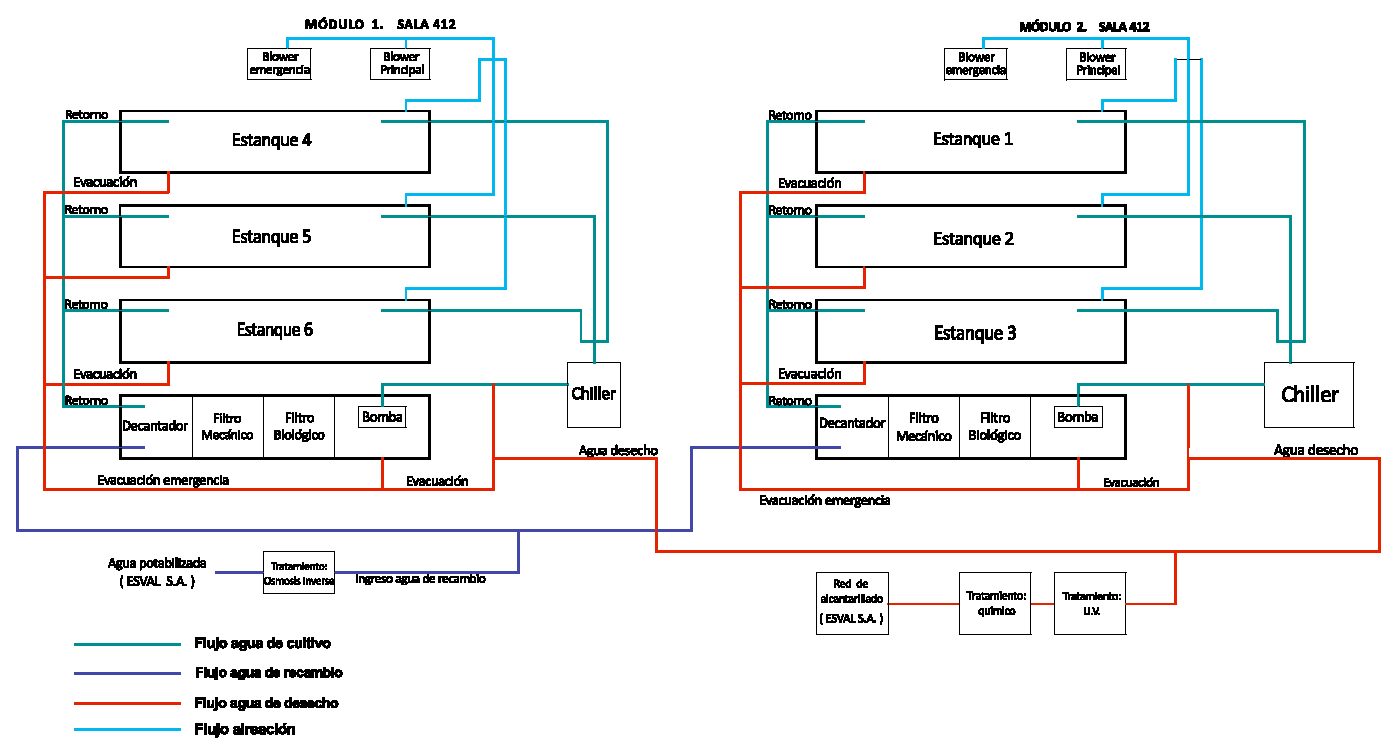
\includegraphics[width=1\textwidth]{ciac}
    \caption {Diagrama de flujo Centro de Investigaciones en Acuicultura Curauma}
    \label {fig:ciac}
\end{figure}

\begin{figure}[h!]
    \centering
    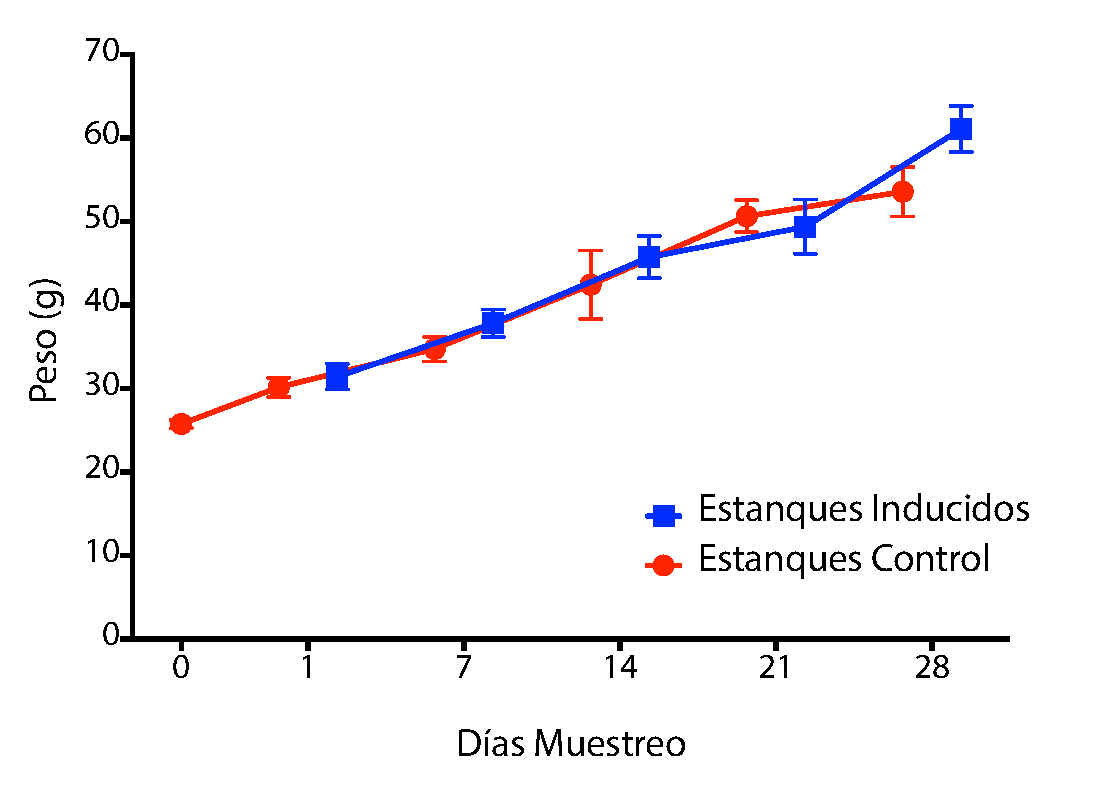
\includegraphics[width=10cm]{peso}
    \caption {Crecimiento promedio de truchas en estudio}
    \label {fig:pesos}
\end{figure}

No se observó ningún cambio significativo entre los pesos registrados
para la dieta control y la dieta suplementada con Zimosán (Figura
\ref{fig:pesos}), lo que indica que este \(\beta\)-glucano no genera un
crecimiento a nivel de masa muscular comparado con el grupo sin
tratamiento.

\clearpage

\epigraph{\textbf{Objetivo 2}: ``Evaluar la expresión de moléculas efectoras y reguladoras de respuesta inmune en tejido branquial de \emph{O.mykiss} tratados con Zymosán A liberado en dieta.''}

\section{Extracción y Cuantificación de RNA}

Para cada una de las muestras realizadas se obtuvo las siguientes
cuantificaciones de RNA (Tabla \ref{tablaRNA}).

\begin{table}[h!]
    \begin{center}
        \begin{threeparttable}
            \caption{Concentraciones de RNA total extraído}\label{tablaRNA}
            \begin{tabular}{l r l r l r l r l r}
                \toprule
                \textbf{ID}   & \textbf{ng/µL} & \textbf{ID} & \textbf{ng/µL} & \textbf{ID} & \textbf{ng/µL} & \textbf{ID} & \textbf{ng/µL} & \textbf{ID} & \textbf{ng/µL}\\
                \midrule
                B1    & 151,40 & B21 & 257,00 & B31 & 242,10 & B41 & 40,20 & B51 & 264,10 \\
                B2 & 63,30 & B22 & 341,50 & B32 & 250,40 & B42 & 121,90 & B52 & 183,00 \\
                B3 & 208,40 & B23 & 145,10 & B33 & 264,10 & B43 & 105,20 & B53 & 393,40 \\
                B4 & 178,30 & B24 & 121,30 & B34 & 295,10 & B44 & 237,30 & B54 & 292,80 \\
                B5 & 248,40 & B25 & 151,70 & B35 & 572,70 & B45 & 116,40 & B55 & 322,60 \\
                B16 & 165,10 & B26 & 326,30 & B36 & 115,60 & B46 & 415,60 & \\
                B17 & 249,90 & B27 & 149,30 & B37 & 183,20 & B47 & 220,80 & \\
                B18 & 138,40 & B28 & 263,90 & B38 & 171,60 & B48 & 271,40 & \\
                B19 & 169,60 & B29 & 357,30 & B39 & 194,50 & B49 & 173,80 & \\
                B20 & 690,70 & B30 & 341,80 & B40 & 192,40 & B50 & 315,40 & \\
                \bottomrule
            \end{tabular}
        \end{threeparttable}
    \end{center}
\end{table}

Las muestras dispuestas en la tabla \ref{tablaRNA} fueron llevadas para
la obtención de cDNA. \section{Estandarización de Partidores}

Para cada molécula en estudio se obtuvieron las siguientes
estandarizaciones de partidores.

\subsection{EF-1$\alpha$}

Se obtuvo la mejor curva estándar, eficiencia y curva de fusión a los
58ºC (Figura \ref{fig:ef1a}).

\begin{figure}[h]
    \centering
        \subcaptionbox{Amplificación\label{fig:ef1a:ampl}}
        {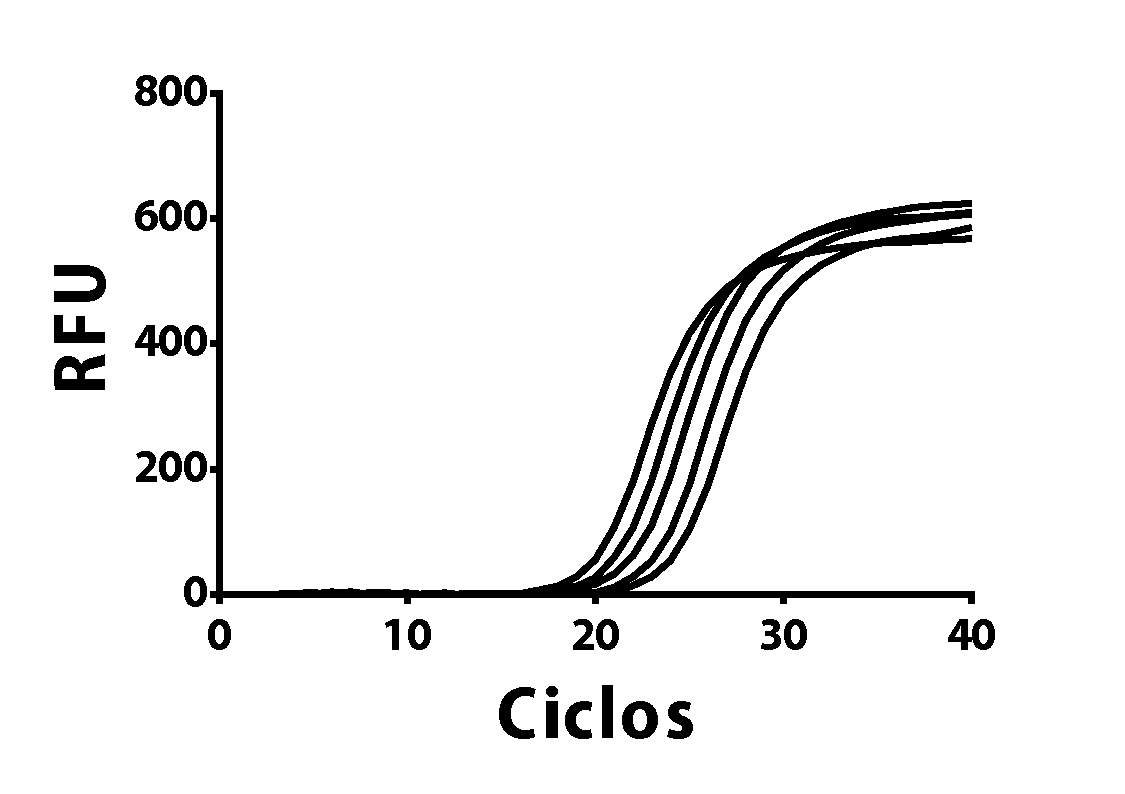
\includegraphics[width=0.32\textwidth]{standarization/ef1a/ampl}}
        \subcaptionbox{Estandarización\label{fig:ef1a:stand}}
        {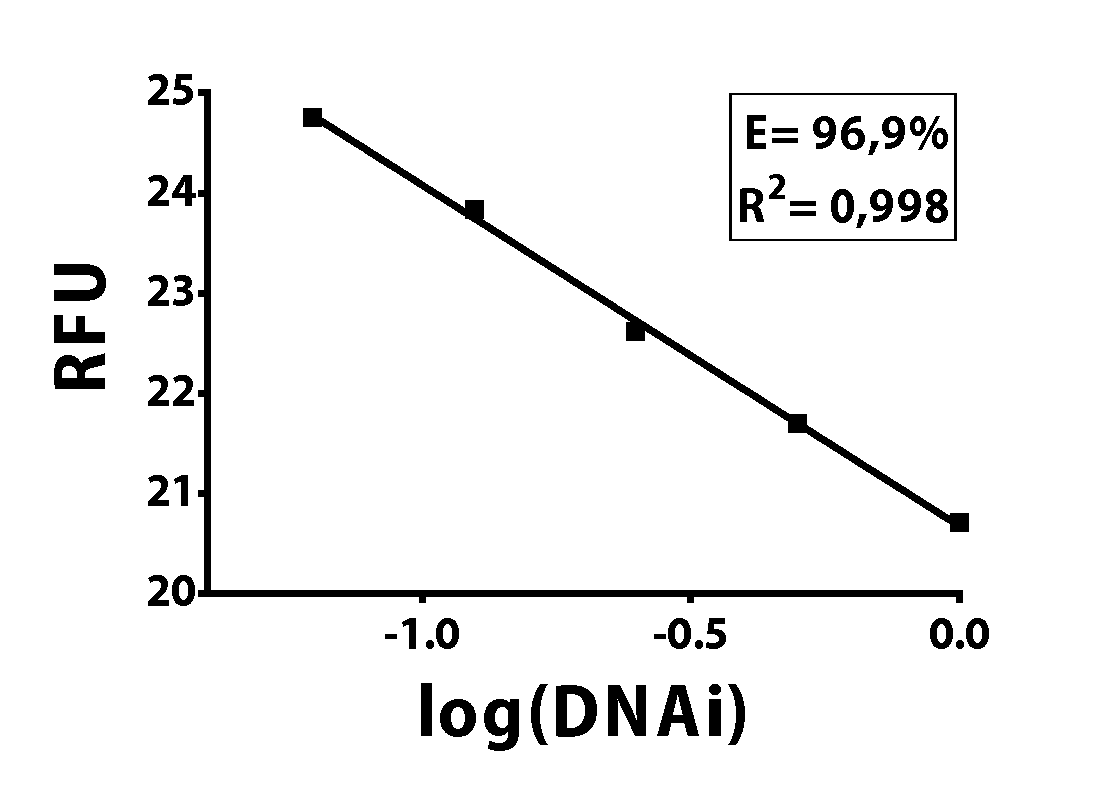
\includegraphics[width=0.32\textwidth]{standarization/ef1a/stand}}
        \subcaptionbox{Disociación\label{fig:ef1a:melting}}
        {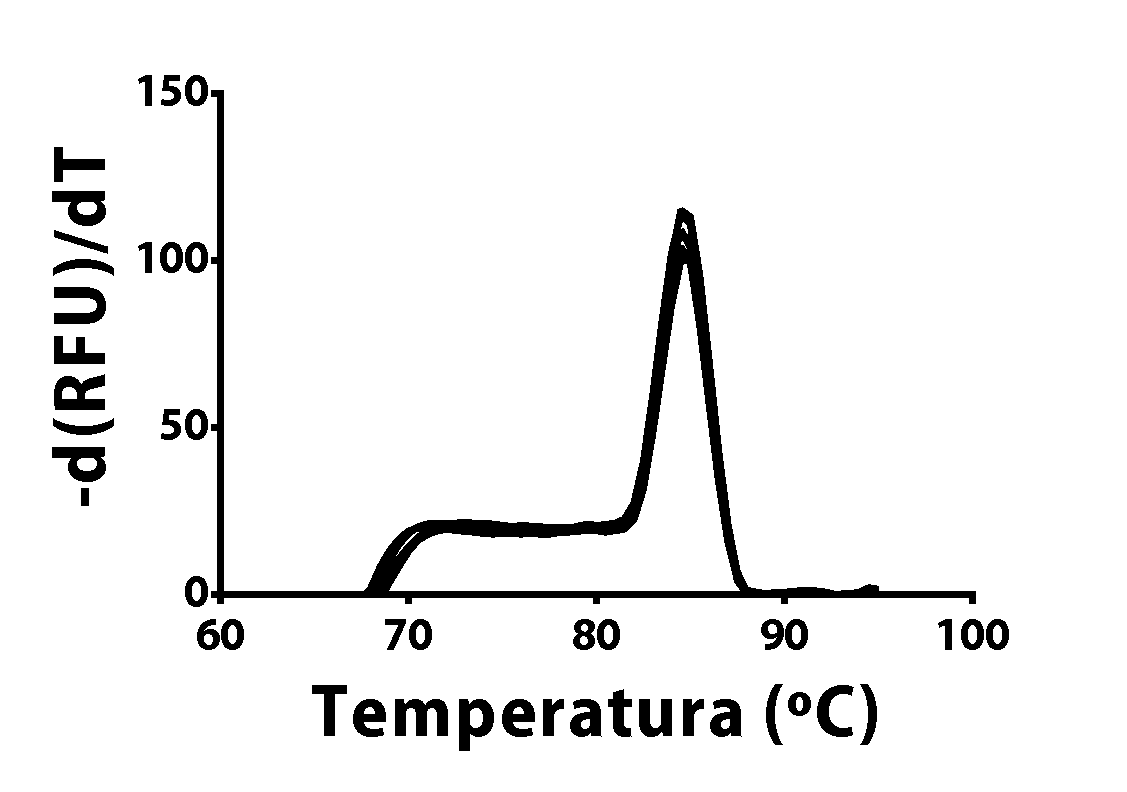
\includegraphics[width=0.32\textwidth]{standarization/ef1a/melting}}
        \caption{Curvas de estandarización del partidor para EF-1$\alpha$}
    \label {fig:ef1a}
\end{figure}

\subsection{IL-12}

Se obtuvo la mejor curva estándar, eficiencia y curva de fusión a los
58ºC. (Figura \ref{fig:il12})

\begin{figure}[h!]
    \centering
        \subcaptionbox{Amplificación\label{fig:il12:ampl}}
        {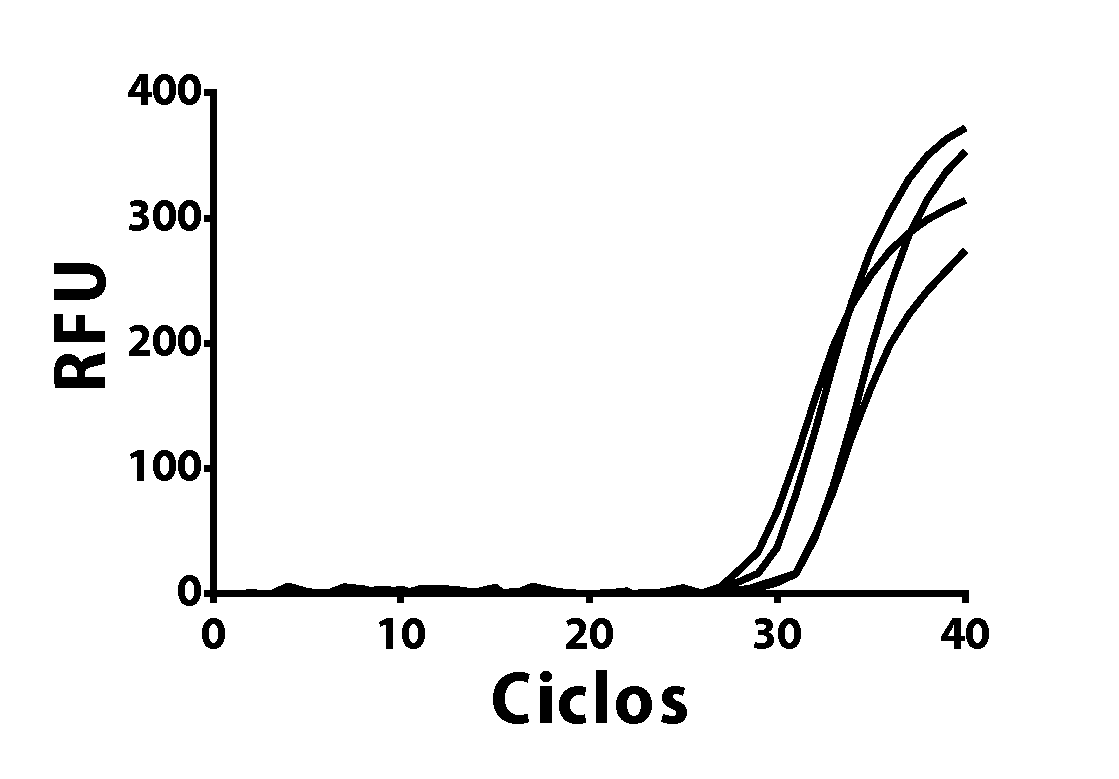
\includegraphics[width=0.32\textwidth]{standarization/il12/ampl}}
        \subcaptionbox{Estandarización\label{fig:il12:stand}}
        {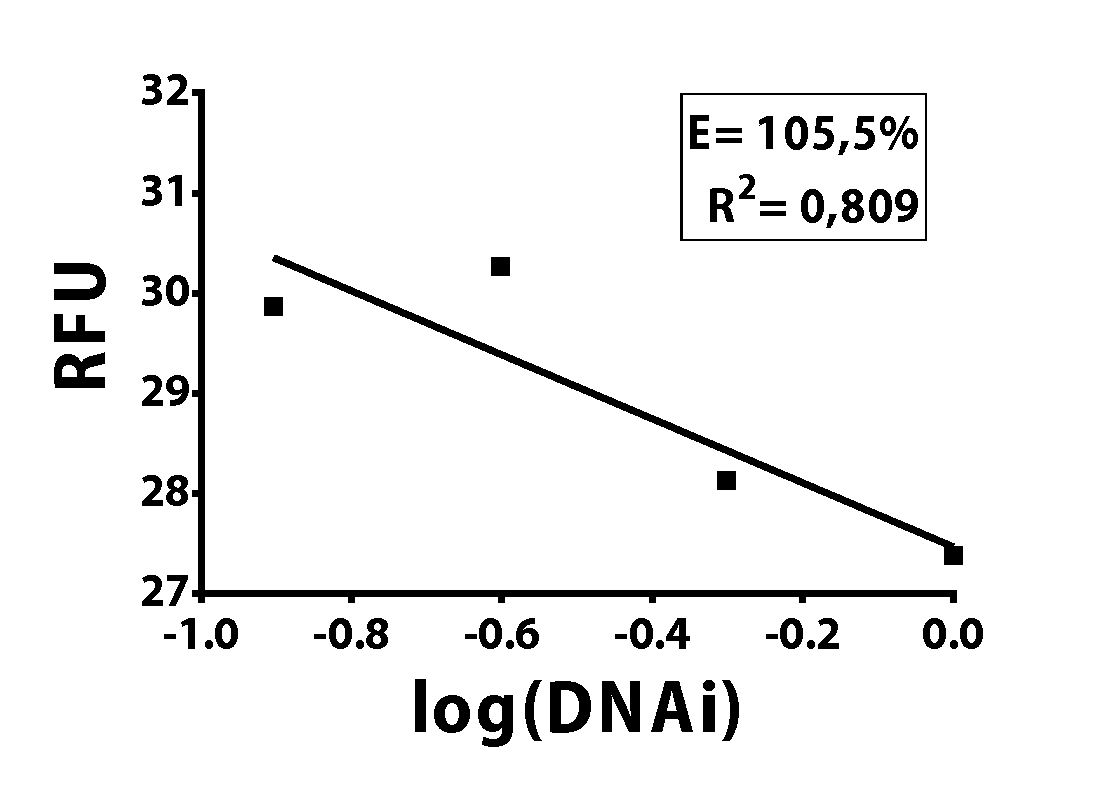
\includegraphics[width=0.32\textwidth]{standarization/il12/stand}}
        \subcaptionbox{Disociación\label{fig:il12:melting}}
        {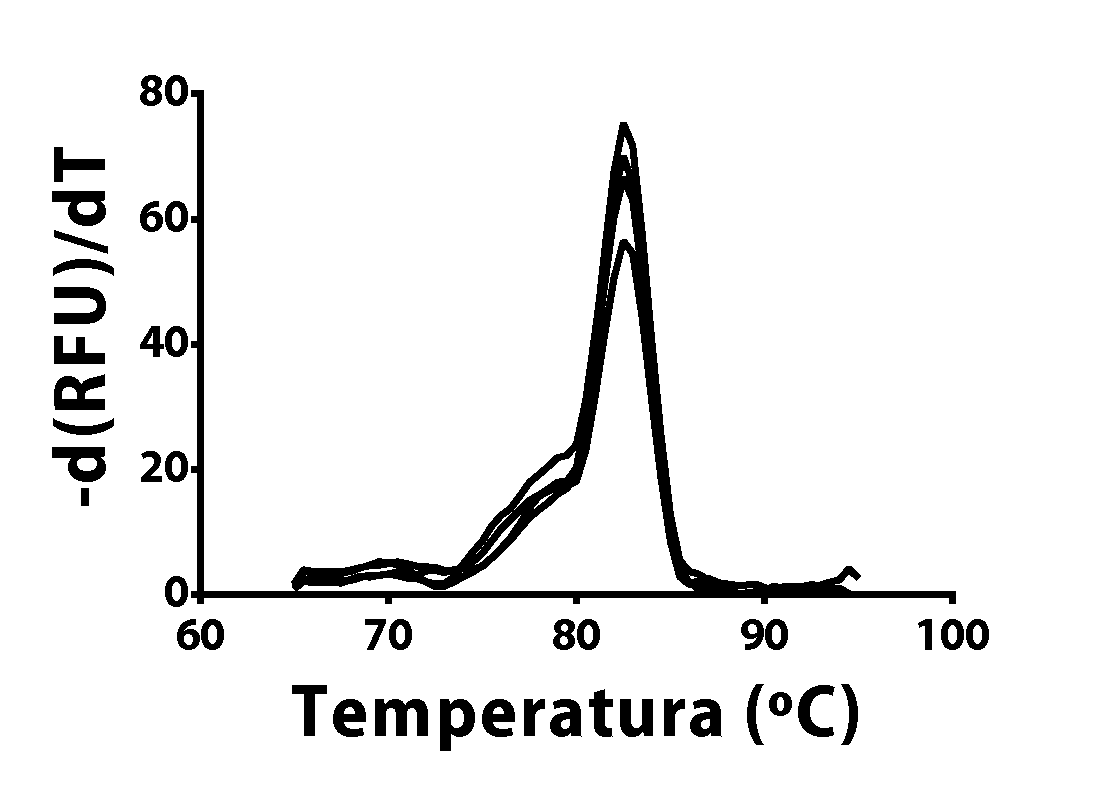
\includegraphics[width=0.32\textwidth]{standarization/il12/melting}}
        \caption{Curvas de estandarización del partidor para IL-12}
        \label {fig:il12}
\end{figure}

\subsection{TNF-$\alpha$}

Se obtuvo la mejor curva estándar, eficiencia y curva de fusión a los
58ºC (Figura \ref{fig:tnfa}).

\begin{figure}[h!]
\centering
   \subcaptionbox{Amplificación\label{fig:tnfa:ampl}}
        {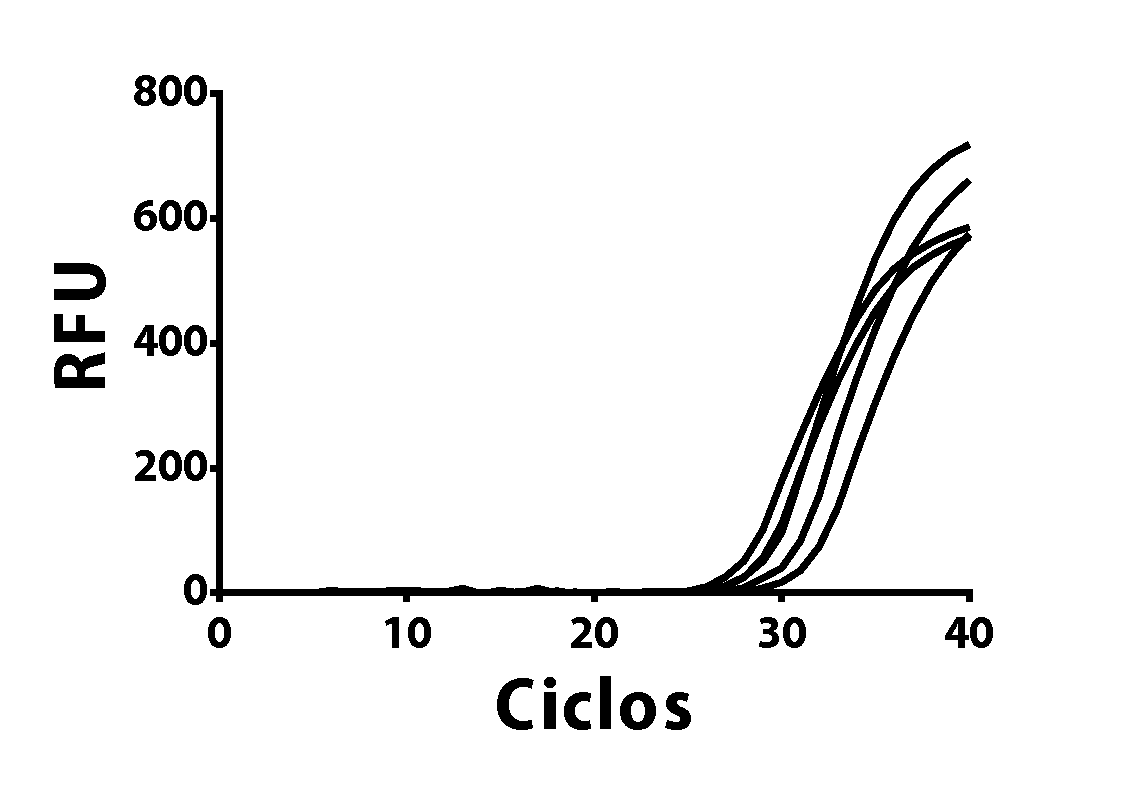
\includegraphics[width=0.32\textwidth]{standarization/tnfa/ampl}}
        \subcaptionbox{Estandarización\label{fig:tnfa:stand}}
        {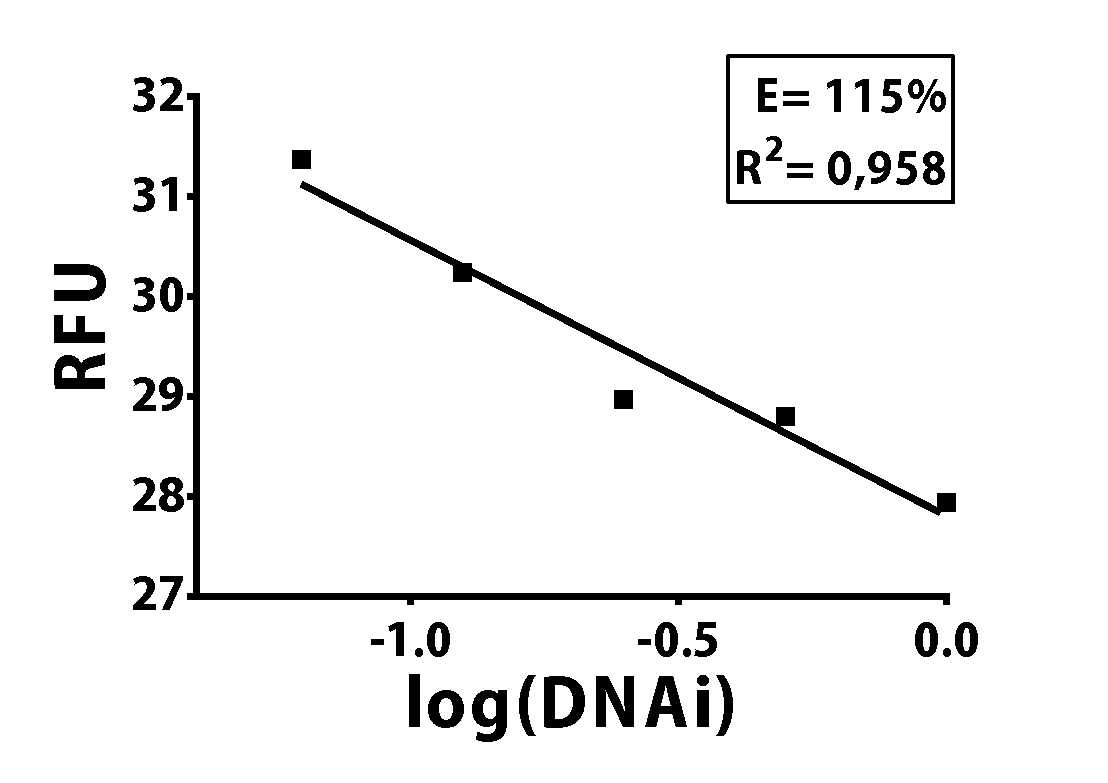
\includegraphics[width=0.32\textwidth]{standarization/tnfa/stand}}
        \subcaptionbox{Disociación\label{fig:tnfa:melting}}
        {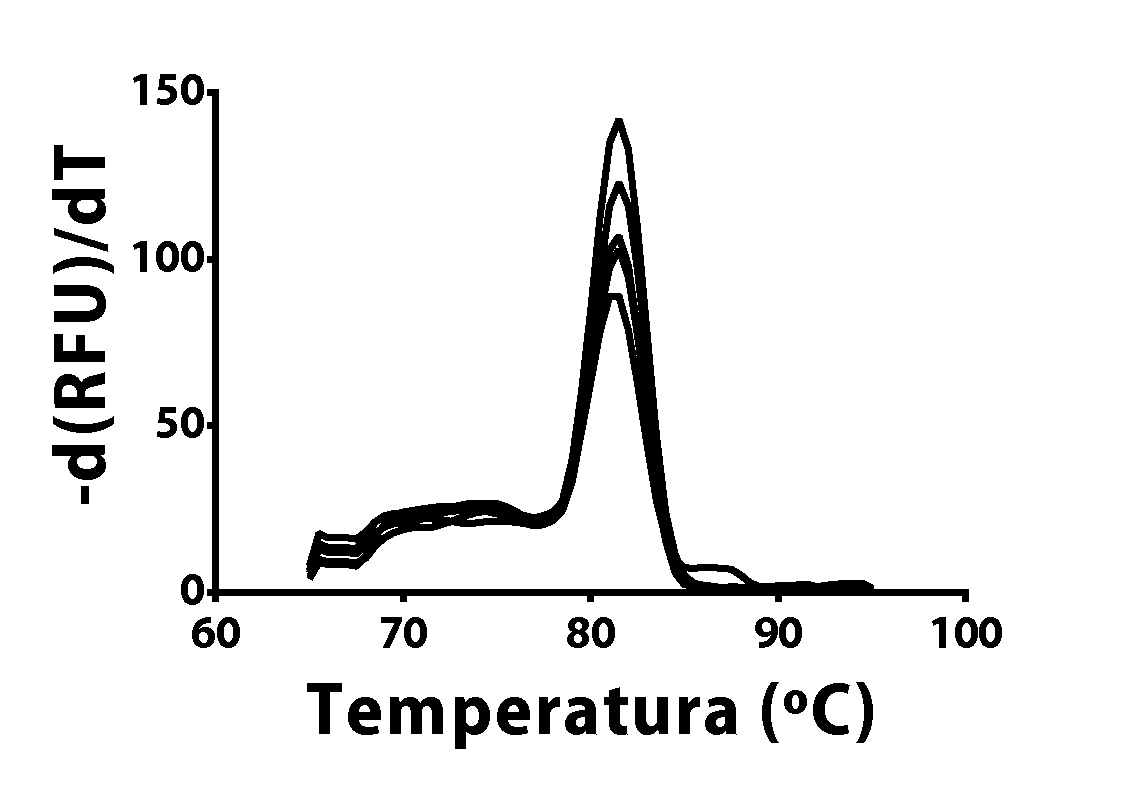
\includegraphics[width=0.32\textwidth]{standarization/tnfa/melting}}
        \caption{Curvas de estandarización del partidor para TNF-$\alpha$}
    \label {fig:tnfa}
\end{figure}

\subsection{IFN-$\gamma$}

Se obtuvo la mejor curva estándar, eficiencia y curva de fusión a los
61.5ºC (Figura \ref{fig:ifng}).

\begin{figure}[h!]
\centering
        \subcaptionbox{Amplificación\label{fig:ifng:ampl}}
        {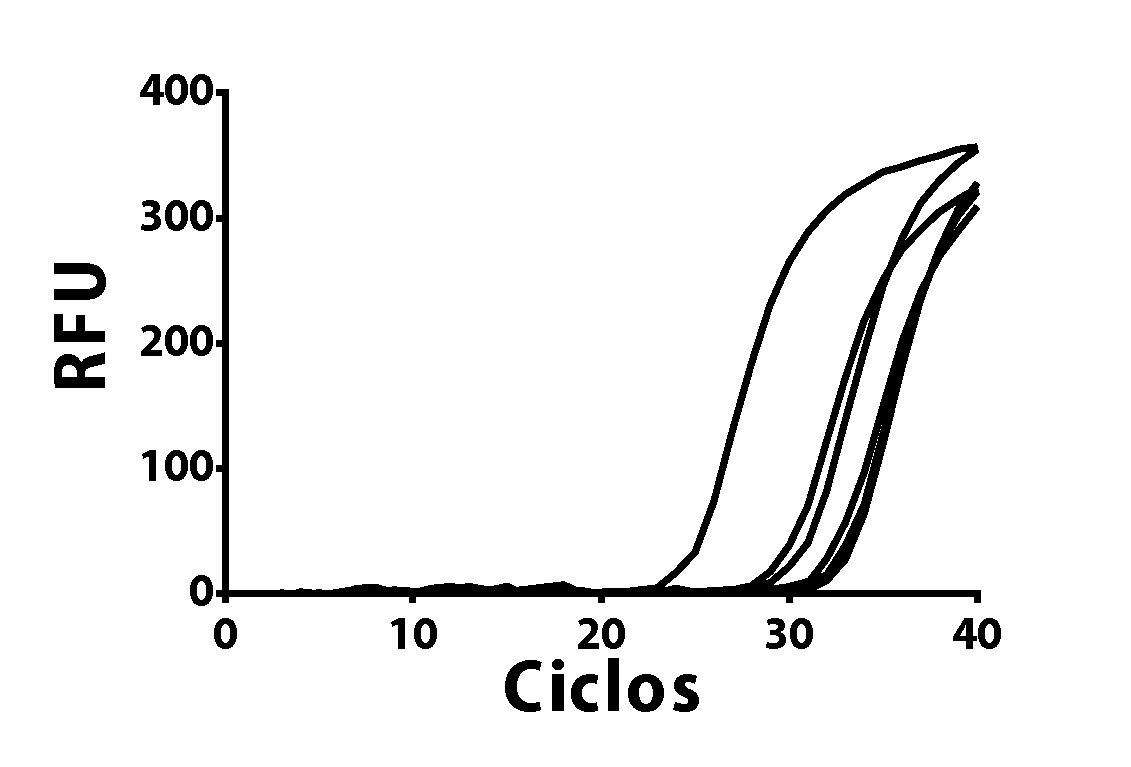
\includegraphics[width=0.32\textwidth]{standarization/ifng/ampl}}
        \subcaptionbox{Estandarización\label{fig:ifng:stand}}
        {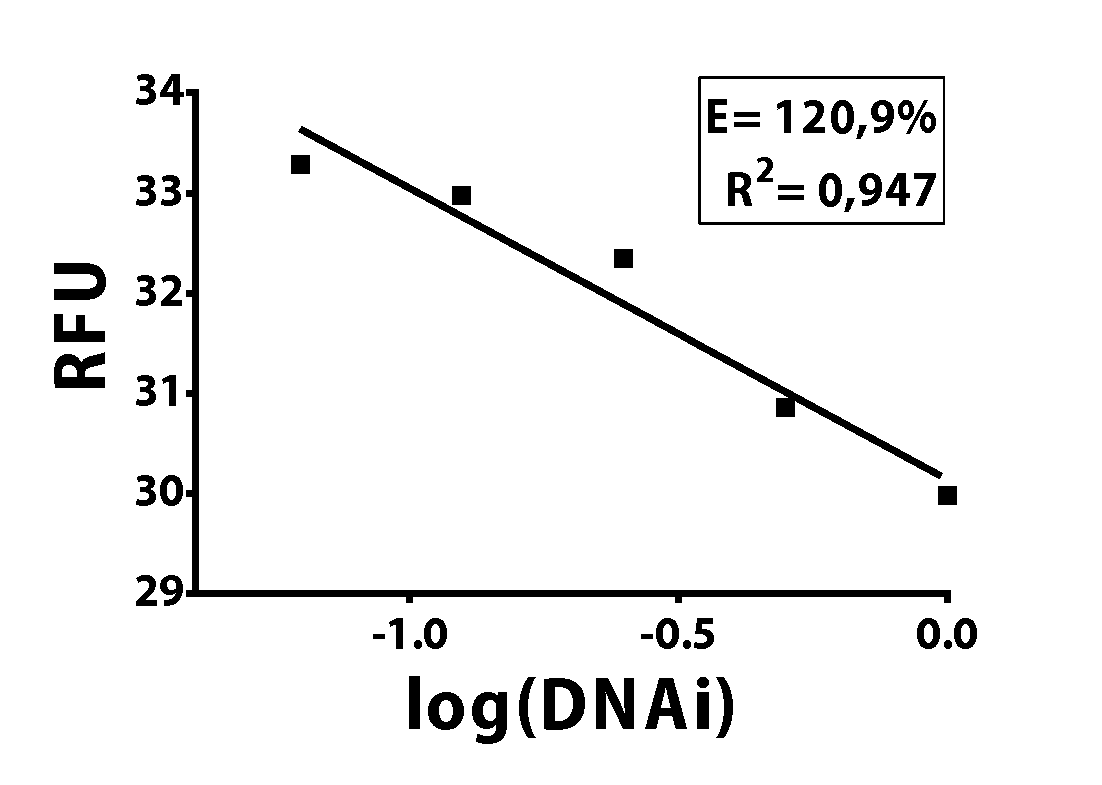
\includegraphics[width=0.32\textwidth]{standarization/ifng/stand}}
        \subcaptionbox{Disociación\label{fig:ifng:melting}}
        {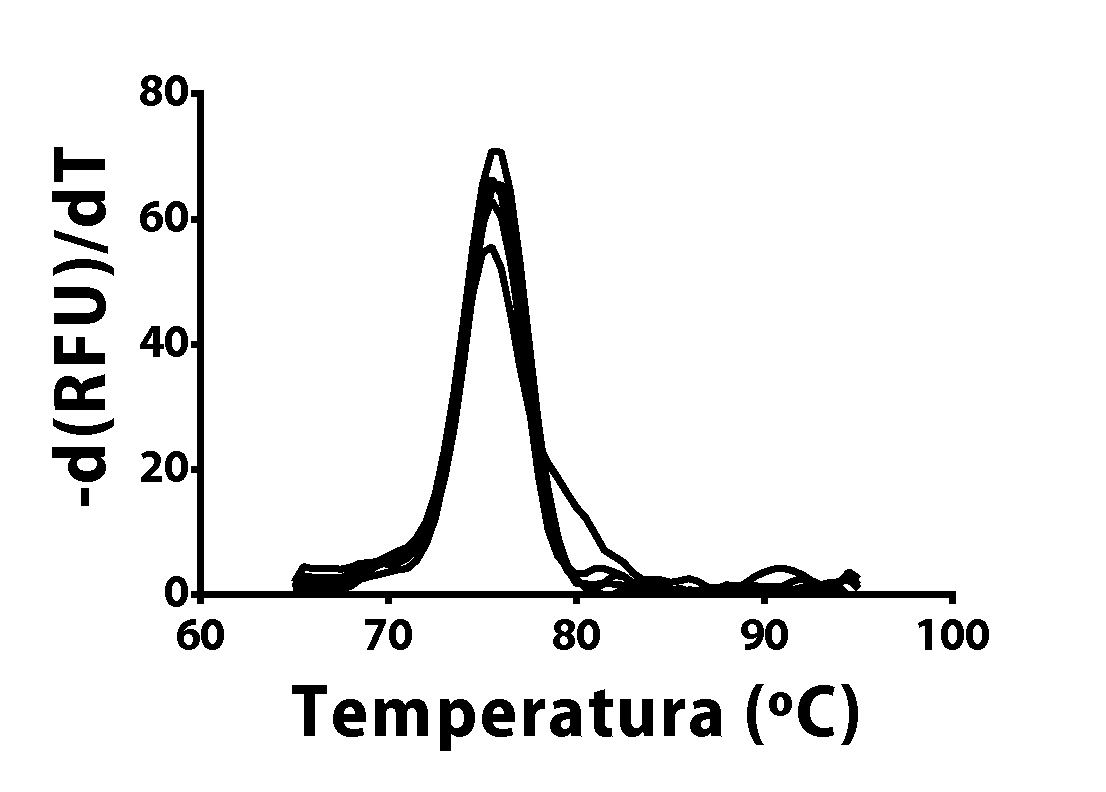
\includegraphics[width=0.32\textwidth]{standarization/ifng/melting}}
         \caption{Curvas de estandarización del partidor para IFN-$\gamma$}
         \label {fig:ifng}
    \end{figure}

\subsection{IL-1$\beta$}

Se obtuvo la mejor curva estándar, eficiencia y curva de fusión a los
58ºC (Figura \ref{fig:il1b}).

\begin{figure}[h!]
\centering
   \subcaptionbox{Amplificación\label{fig:il1b:ampl}}
        {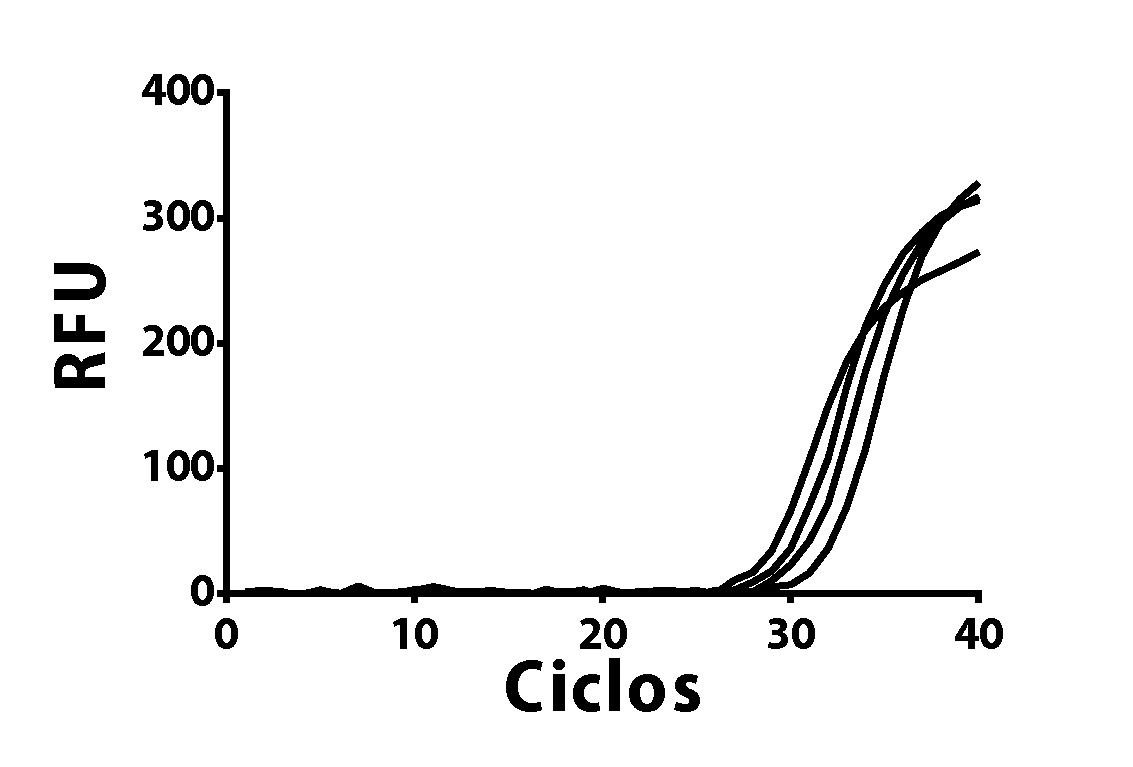
\includegraphics[width=0.32\textwidth]{standarization/il1b/ampl}}
        \subcaptionbox{Estandarización\label{fig:il1b:stand}}
        {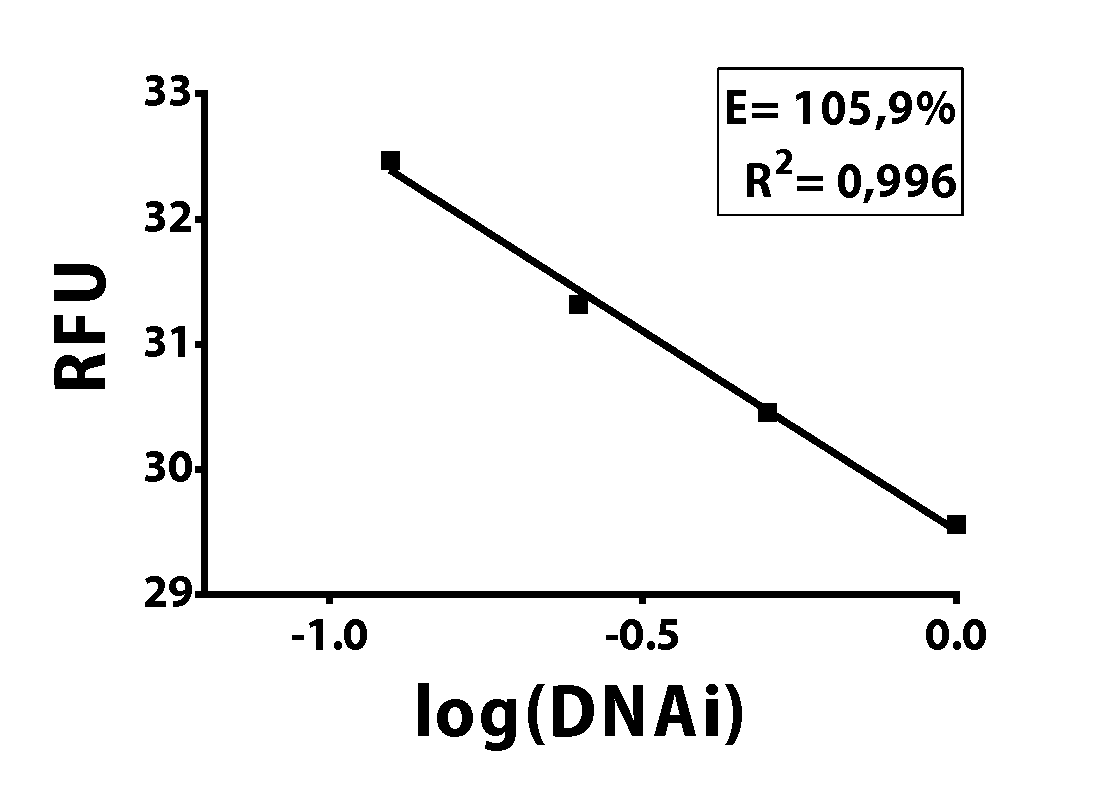
\includegraphics[width=0.32\textwidth]{standarization/il1b/stand}}
        \subcaptionbox{Disociación\label{fig:il1b:melting}}
        {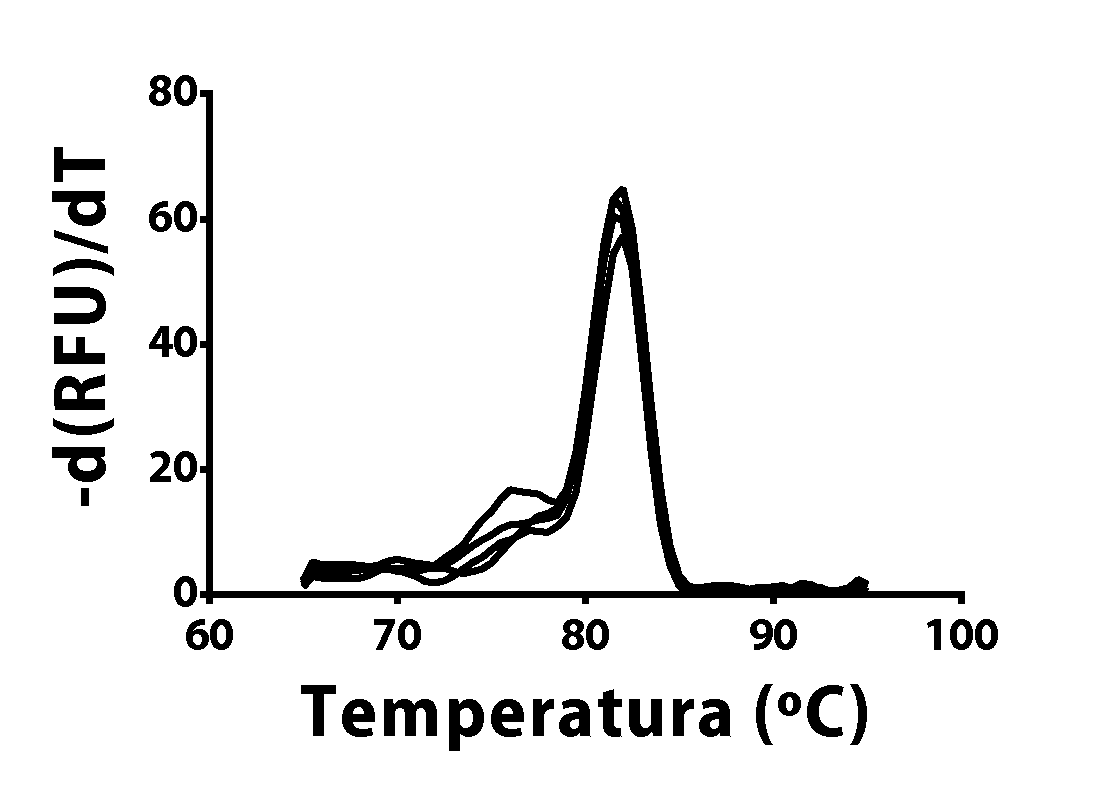
\includegraphics[width=0.32\textwidth]{standarization/il1b/melting}}
        \caption{Curvas de estandarización del partidor para IL-1$\beta$}
    \label {fig:il1b}
\end{figure}

\subsection{iNOS}

Se obtuvo la mejor curva estándar, eficiencia y curva de fusión a los
58ºC (Figura \ref{fig:inos}).

\begin{figure}[h!]
\centering
   \subcaptionbox{Amplificación\label{fig:inos:ampl}}
        {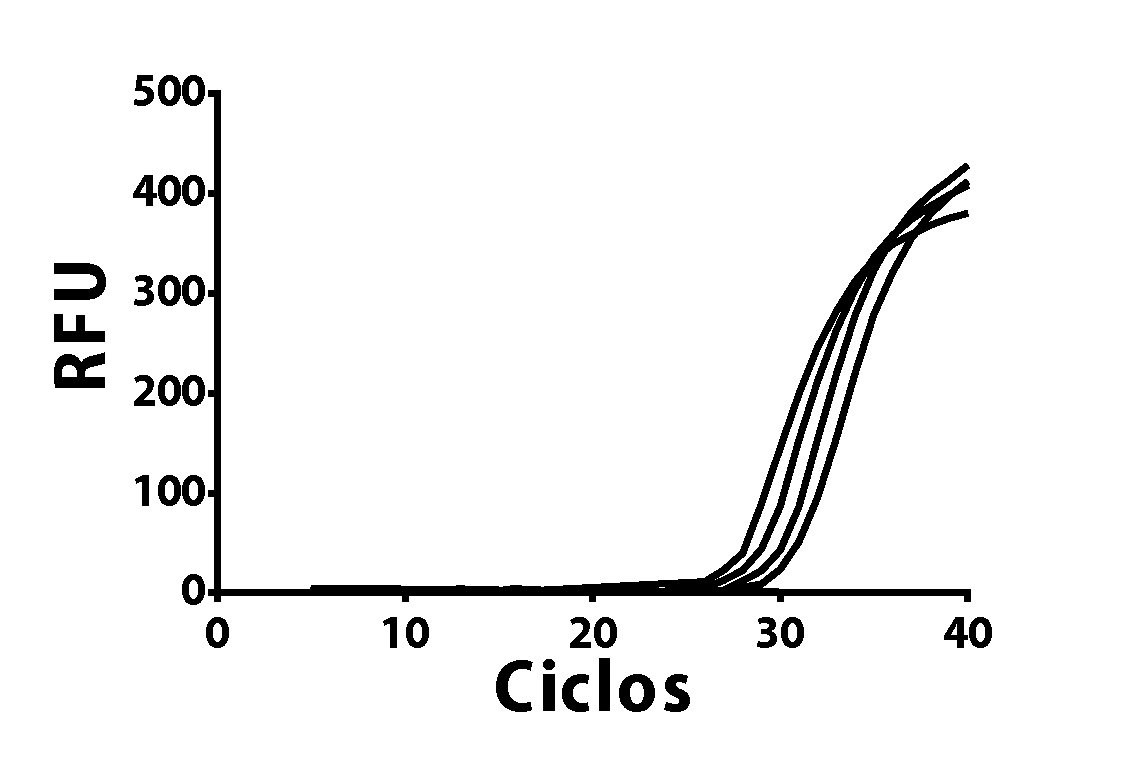
\includegraphics[width=0.32\textwidth]{standarization/inos/ampl}}
        \subcaptionbox{Estandarización\label{fig:inos:stand}}
        {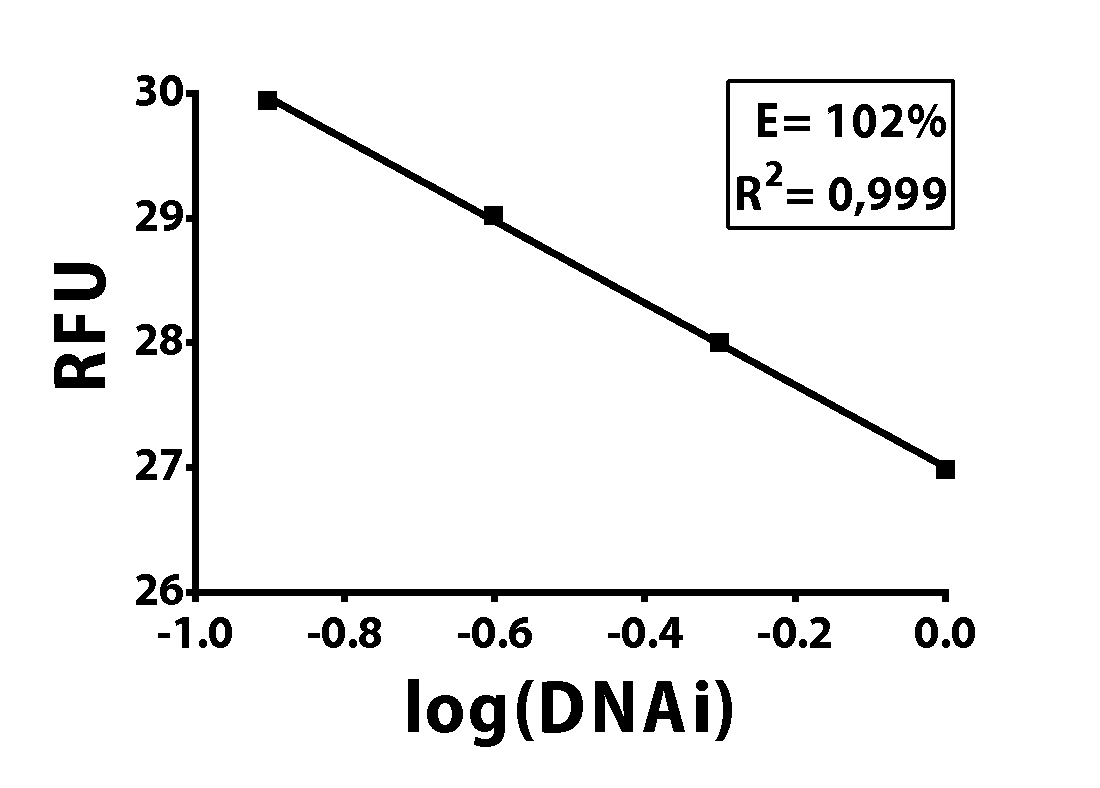
\includegraphics[width=0.32\textwidth]{standarization/inos/stand}}
        \subcaptionbox{Disociación\label{fig:inos:melting}}
        {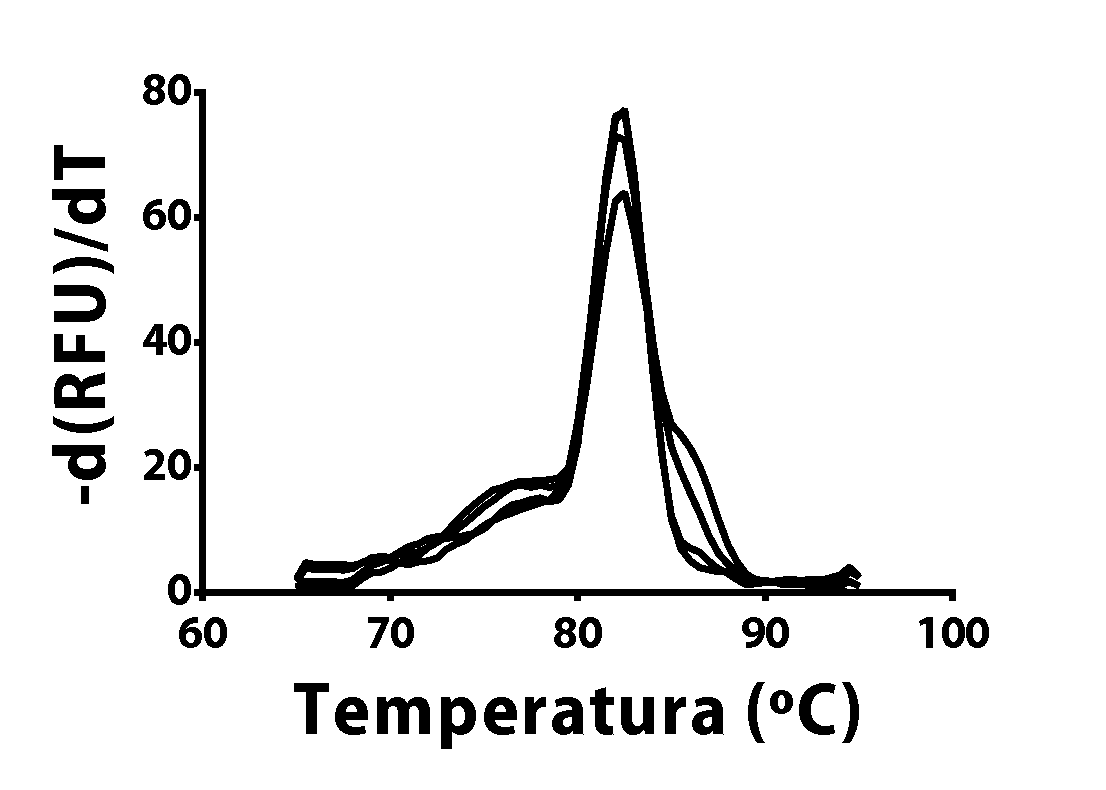
\includegraphics[width=0.32\textwidth]{standarization/inos/melting}}
        \caption{Curvas de estandarización del partidor para iNOS}
    \label {fig:inos}
\end{figure}

\begin{table}[h!]
    \centering
    \begin{threeparttable}
        \caption{Síntesis: Temperaturas de annealing estandarizadas para cada partidor} \label{tabla:sintesispartidores}
        \begin{tabularx}{0.5\textwidth}{X l}
            \toprule
            Partidor & TA \\
            \midrule
            EF-1$\alpha$ & 58ºC \\
            IL-1$\beta$ & 58ºC \\
            TNF-$\alpha$ & 58ºC \\
            IFN-$\gamma$ & 61,5ºC \\
            iNOS & 58ºC \\
            \bottomrule
        \end{tabularx}
    \begin{tablenotes}
        \item $T_A$= Temperatura de \emph{annealing}
    \end{tablenotes}
    \end{threeparttable}
\end{table}

\section{PCR en tiempo real}

Se procedió a realizar la PCR en tiempo real usando las temperaturas de
annealing obtenidas en la Tabla \ref{tabla:sintesispartidores}.

En todas las muestras el valor de \(C_T\) obtenido para el gen
EF-1\(\alpha\) fue similar, lo que indicó que las amplificaciones se
desarrollaron de forma correcta y que en todas las reacciones se partió
de cantidades similares de cDNA (Figura \ref{qef1a}).

\begin{figure}[h!]
    \centering
    \begin{subfigure}{0.32\textwidth}
        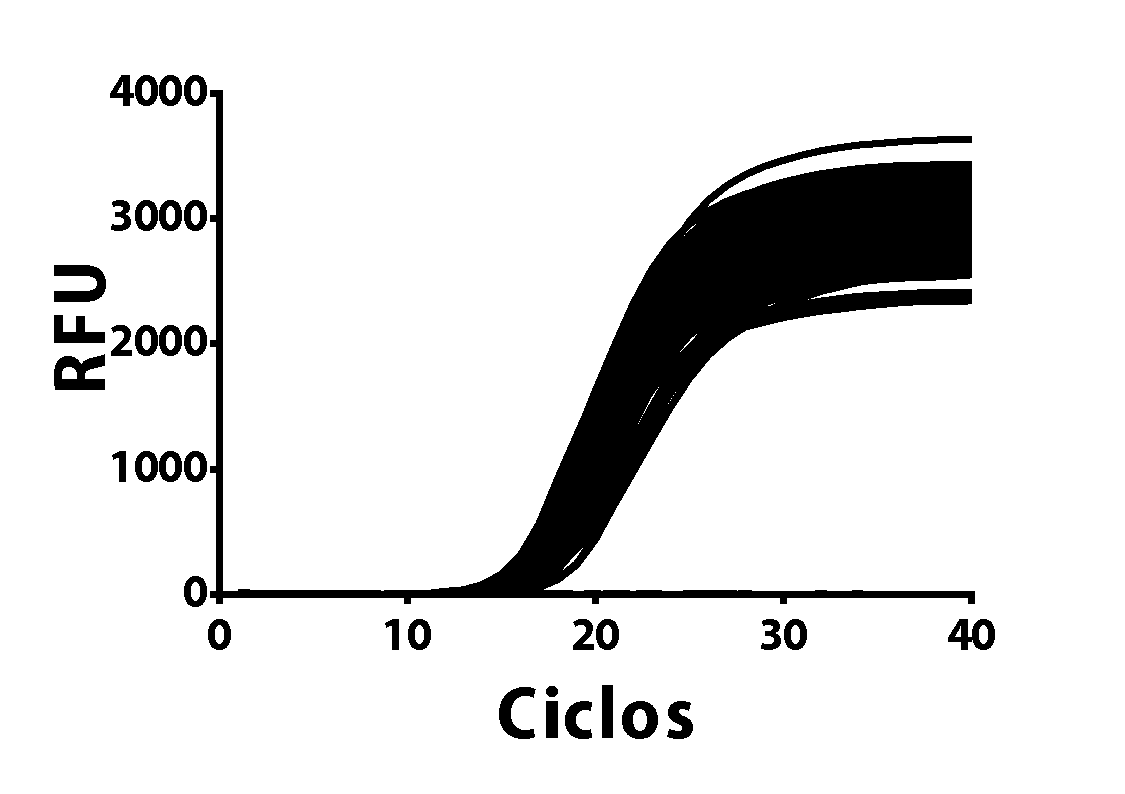
\includegraphics[width=1\textwidth]{qef1a}
        \caption{Curva de amplificación}
        \end{subfigure}
    \begin{subfigure}{0.32\textwidth}
        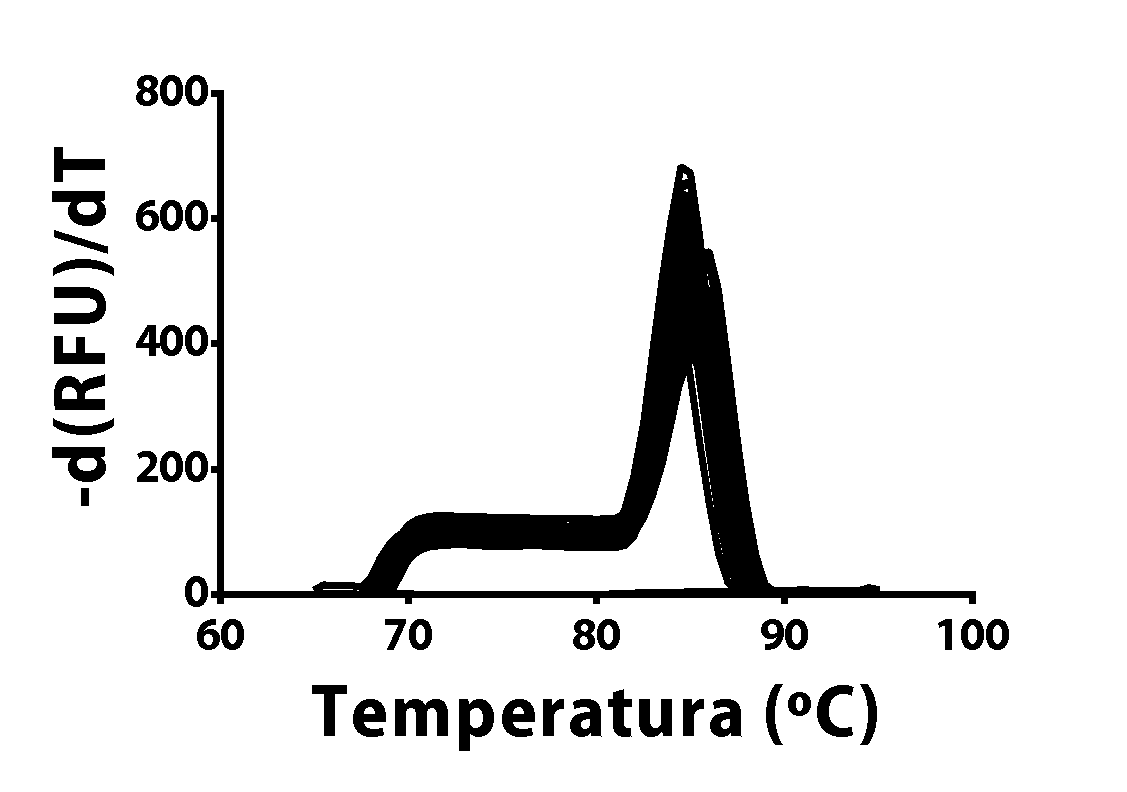
\includegraphics[width=01\textwidth]{qef1am}
        \caption{Curva de disociación}
    \end{subfigure}
    \caption{Reacción de PCR en Tiempo real para el gen de referencia EF-1a}
    \label{qef1a}
\end{figure}

\begin{figure}[h!]
    \begin{subfigure}{0.5\textwidth}
        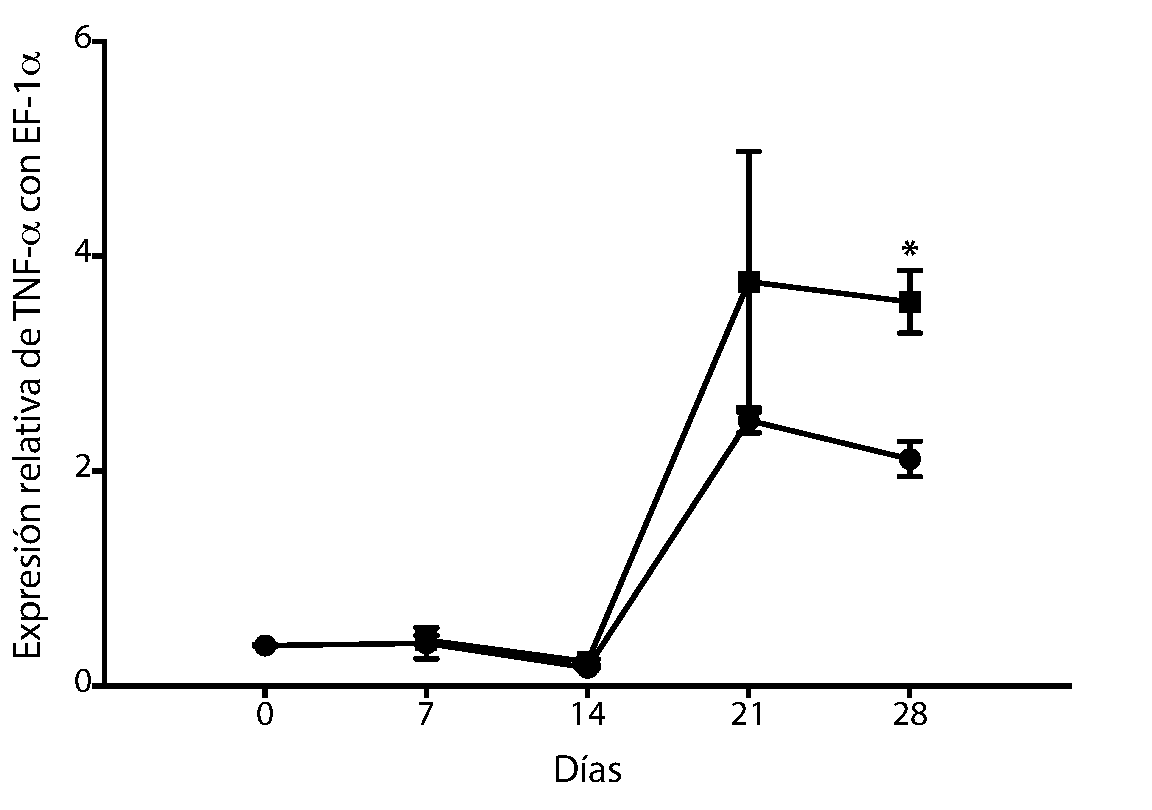
\includegraphics[width=0.9\textwidth]{eps/qPCR/pdf/qtnfa}
        \caption{TNF-$\alpha$}
        \label{fig:qpcr:tnfa}
        \end{subfigure}
    \begin{subfigure}{0.5\textwidth}
        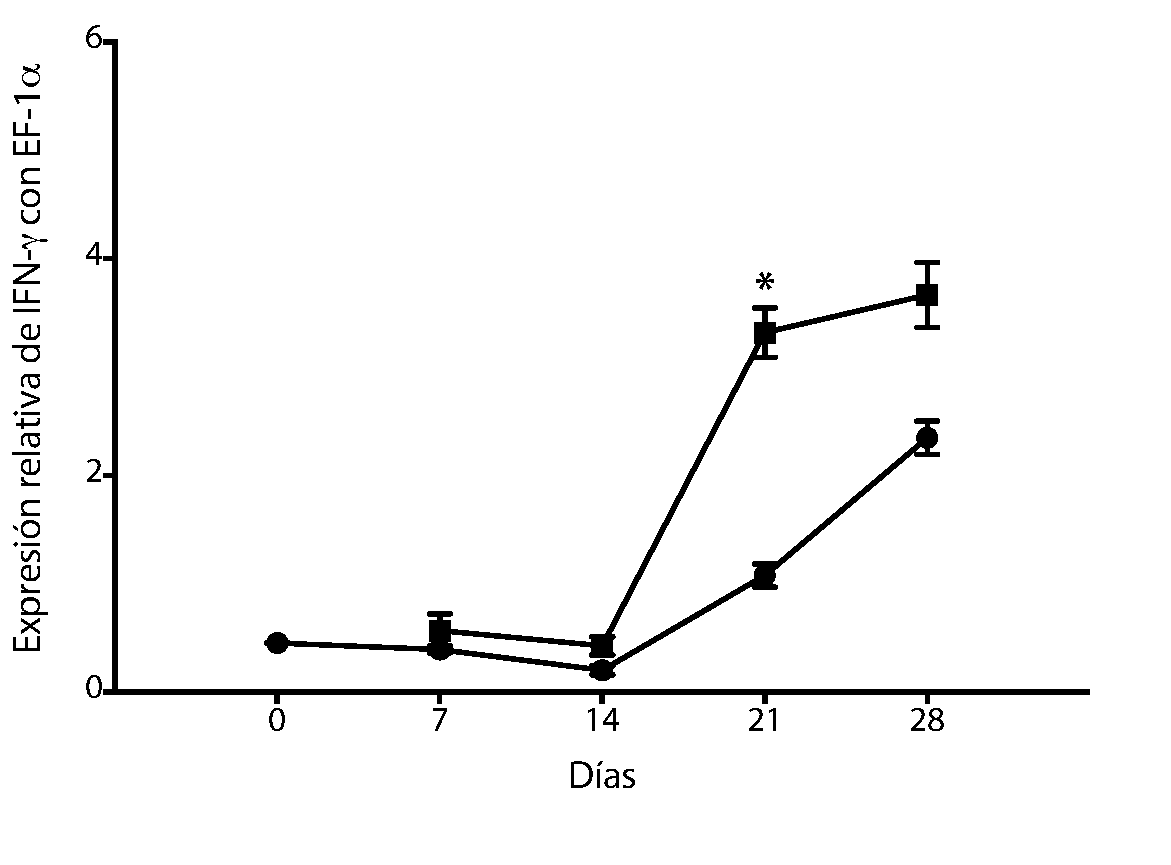
\includegraphics[width=0.9\textwidth]{eps/qPCR/pdf/qifng}
        \caption{IFN-$\gamma$}
        \label{fig:qpcr:ifng}
    \end{subfigure}
    \begin{subfigure}{0.5\textwidth}
        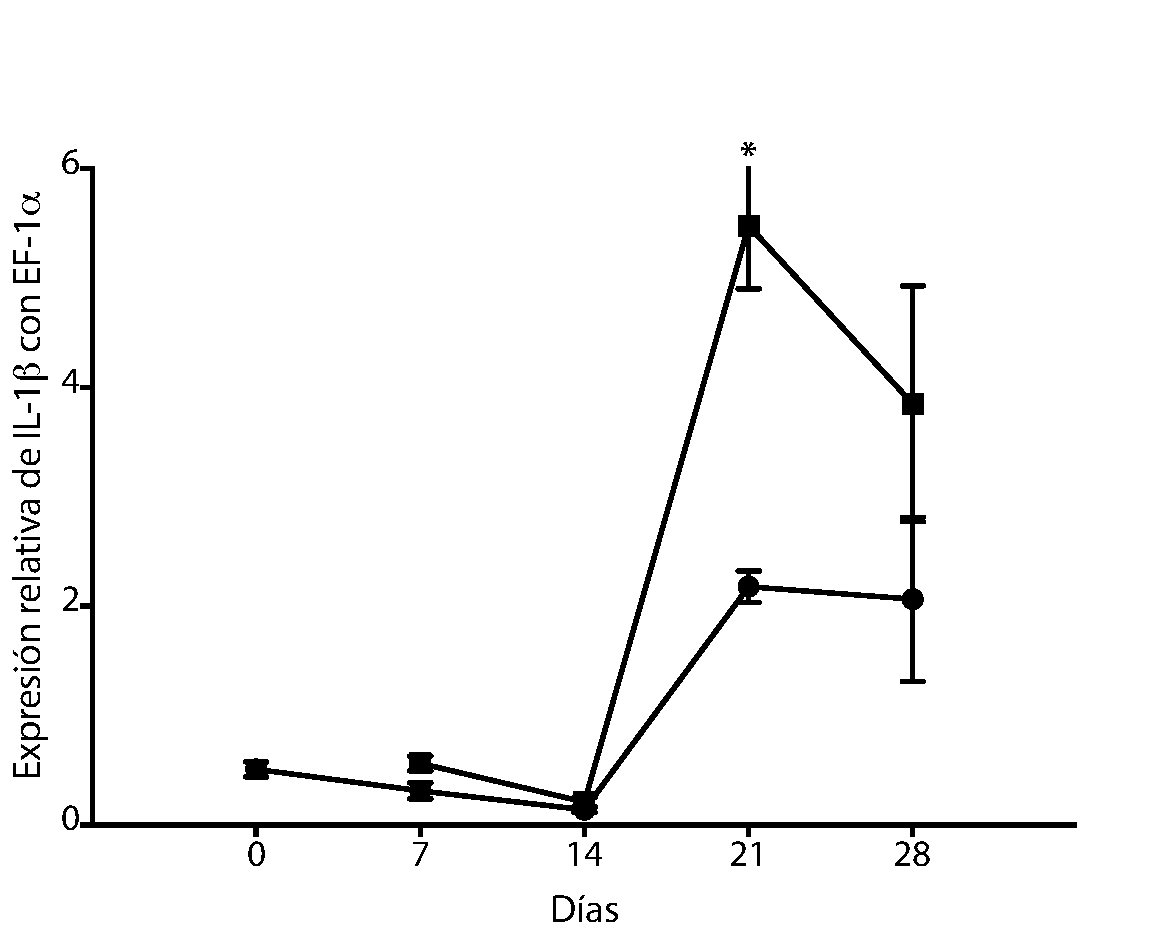
\includegraphics[width=0.9\textwidth]{eps/qPCR/pdf/qil1b}
        \caption{IL-1$\beta$}
        \label{fig:qpcr:il1b}
    \end{subfigure}
    \begin{subfigure}{0.5\textwidth}
        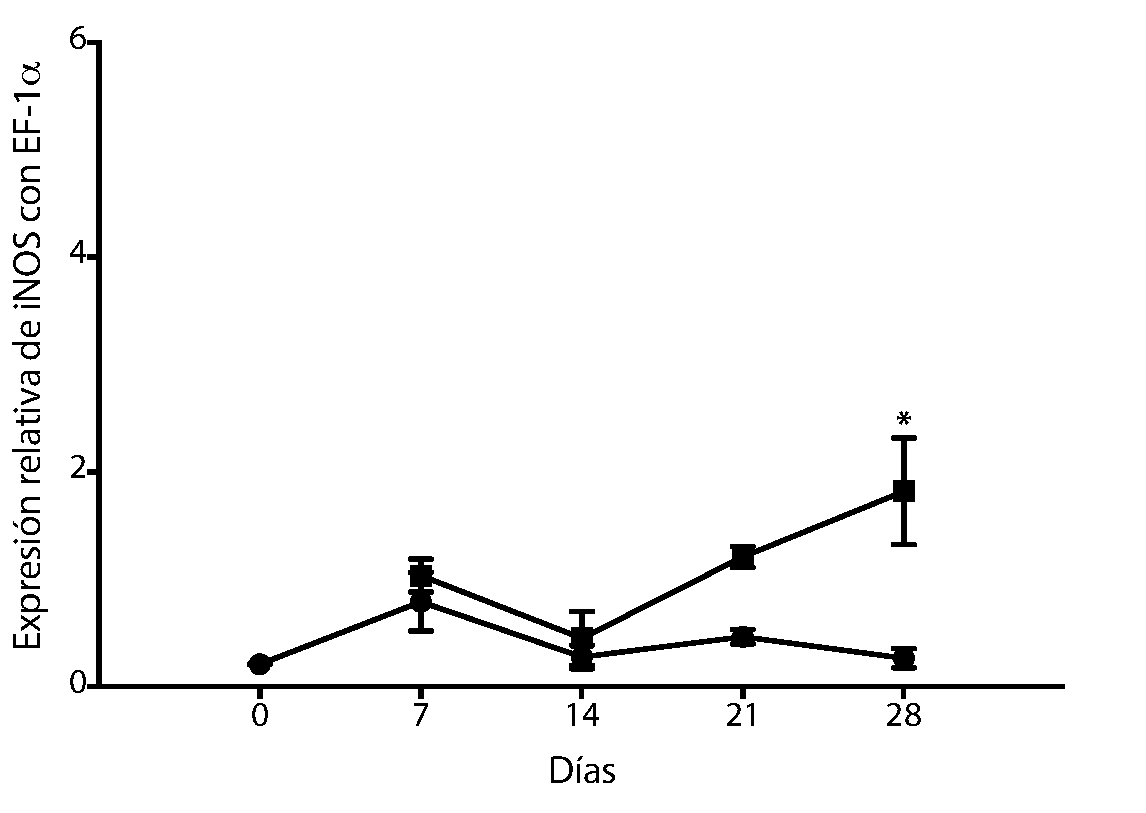
\includegraphics[width=0.9\textwidth]{eps/qPCR/pdf/qinos}
        \caption{iNOS}
        \label{fig:qpcr:inos}
    \end{subfigure}
    \begin{subfigure}{0.5\textwidth}
        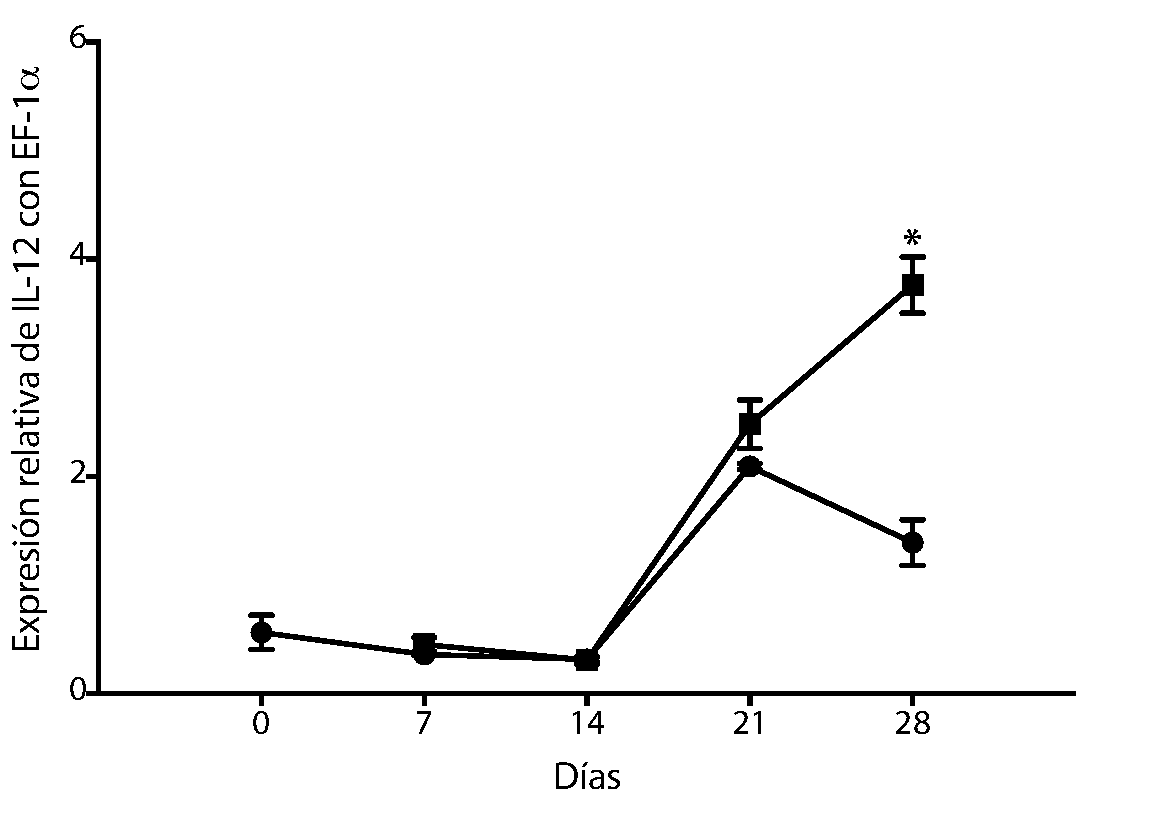
\includegraphics[width=0.9\textwidth]{eps/qPCR/pdf/qil12}
        \caption{IL-12}
        \label{fig:qpcr:il12}
    \end{subfigure}
    \begin{subfigure}{0.5\textwidth}
        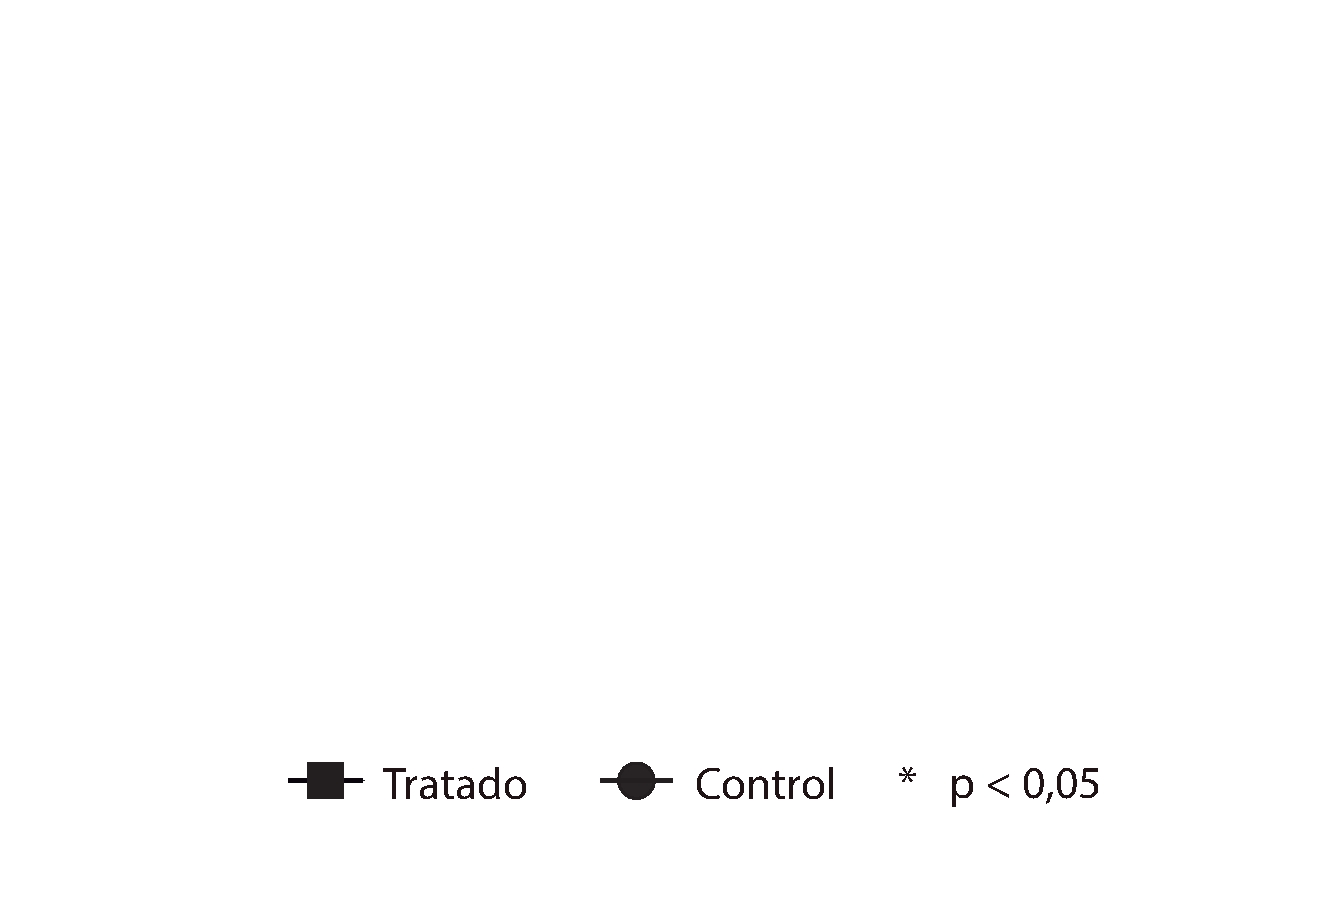
\includegraphics[width=0.9\textwidth]{eps/qPCR/leyenda}
    \end{subfigure}
    \caption{Expresión relativa de los genes en estudio frente a EF-1$\alpha$}
    \label{fig:qpcr}
\end{figure}

\subsection{TNF-$\alpha$}

Para el gen del factor de necrosis tumoral alfa (Figura
\ref{fig:qpcr}\subref{fig:qpcr:tnfa}) la expresión de transcrito se
mantuvo constante en condiciones controles y tratadas hasta el día 14,
donde aumentó súbitamente la cantidad relativa de mensajero en ambas
circunstancias hasta llegar a su máximo \emph{peak} el día 21,
finalmente baja un poco su expresión el día 28, día en el cual hubo una
diferencia significativa con su control(\(p \leq 0,05\)).

\subsection{IFN-$\gamma$}

La expresión relativa del transcrito de Interferón gamma (Figura
\ref{fig:qpcr}\subref{fig:qpcr:ifng}) frente al gen de referencia en
condiciones control y tratadas se mantuvieron en bajas cantidades hasta
el día 14, 7 días después hubo un peak significativo comparado con su
control (\(p \leq 0,05\)), cabe destacar que los días 21 y 28 en
situaciones control hubo un aumento de transcrito para este gen, aunque
no significativo con sus pares tratados.

\subsection{IL-1$\beta$}

Al igual que los dos genes anteriores, la expresión de interleuquina 1
beta (Figura \ref{fig:qpcr}\subref{fig:qpcr:il1b}) se mantuvo baja los
primeros 14 días con respecto al control inicial, para luego el día 21
aumentar súbita y significativamente (\(p \leq 0,05\)) en condiciones
tratadas frente a su control del día, finalmente el día 28 baja la
expresión del transcrito mientras que el control se mantiene estable.

\subsection{iNOS}

El gen de iNOS (Figura \ref{fig:qpcr}\subref{fig:qpcr:inos}) el día 7 se
empezó a transcribir demostrando un aumento en ambas condiciones frente
al control inicial, para luego bajar su expresión casi al nivel del día
0, luego, en condiciones tratadas, este gen experimenta una gran
expresión frente al gen de referencia (\(p \leq 0,05\)), siendo
significativa el día 21, y subiendo hasta el día 28. En los peces
controles, desde el día 14 al 28 se mantuvo prácticamente constante.

\subsection{IL-12}

El comportamiento de Interleuquina 12 (Figura
\ref{fig:qpcr}\subref{fig:qpcr:inos}) tiene cierta tendencia comparado
con la expresión del gen para IL-1\(\beta\), ya que también se gatilla
su expresión el día 14, aunque para el caso de esta citoquina, el día 28
es su mayor \emph{peak} siendo significativo este con respecto a su
control (\(p \leq 0,05\)).

\subsection{Síntesis comparada del estudio}

Las 5 moléculas presentan sobre expresión entre los días 21 y 28.

La molécula que obtuvo una mayor up-regulación fue IL-1\(\beta\),
llegando hasta casi 6 veces su cuantificación relativa frente al gen de
referencia, la que obtuvo una menor up-regulación, aunque igualmente
significativa fue iNOS llegando entre 1.5 a 2 veces de cambio con
respecto al gen de referencia.

El día con mayor sobre-expresión de los genes que codifican para estas
moléculas fue el 21, teniendo up-regulaciones significativas con
respecto a su control para las moléculas: IFN-\(\gamma\), IL-1\(\beta\)
e iNOS, mientras que el día 28 las moléculas que tuvieron una
up-regulación significativa fueron TNF-\(\alpha\) e IL-12.

\clearpage

\epigraph{\textbf{Objetivo 3}: ``Detectar la disponibilidad de proteínas efectoras y reguladoras de respuesta inmune en tejido branquial de O.mykiss tratados con Zymosán A liberado en dieta.''}

\section{Extracción y Cuantificación de Proteínas}

Con los datos obtenidos por el lector espectrofotométrico de
microplacas, usando las concentraciones sembradas de BSA, se construyó
la curva de calibrado para la cuantificación de proteínas. Obteniendo el
siguiente gráfico y ecuación de la recta:

\begin{figure}[h!]
\centering
    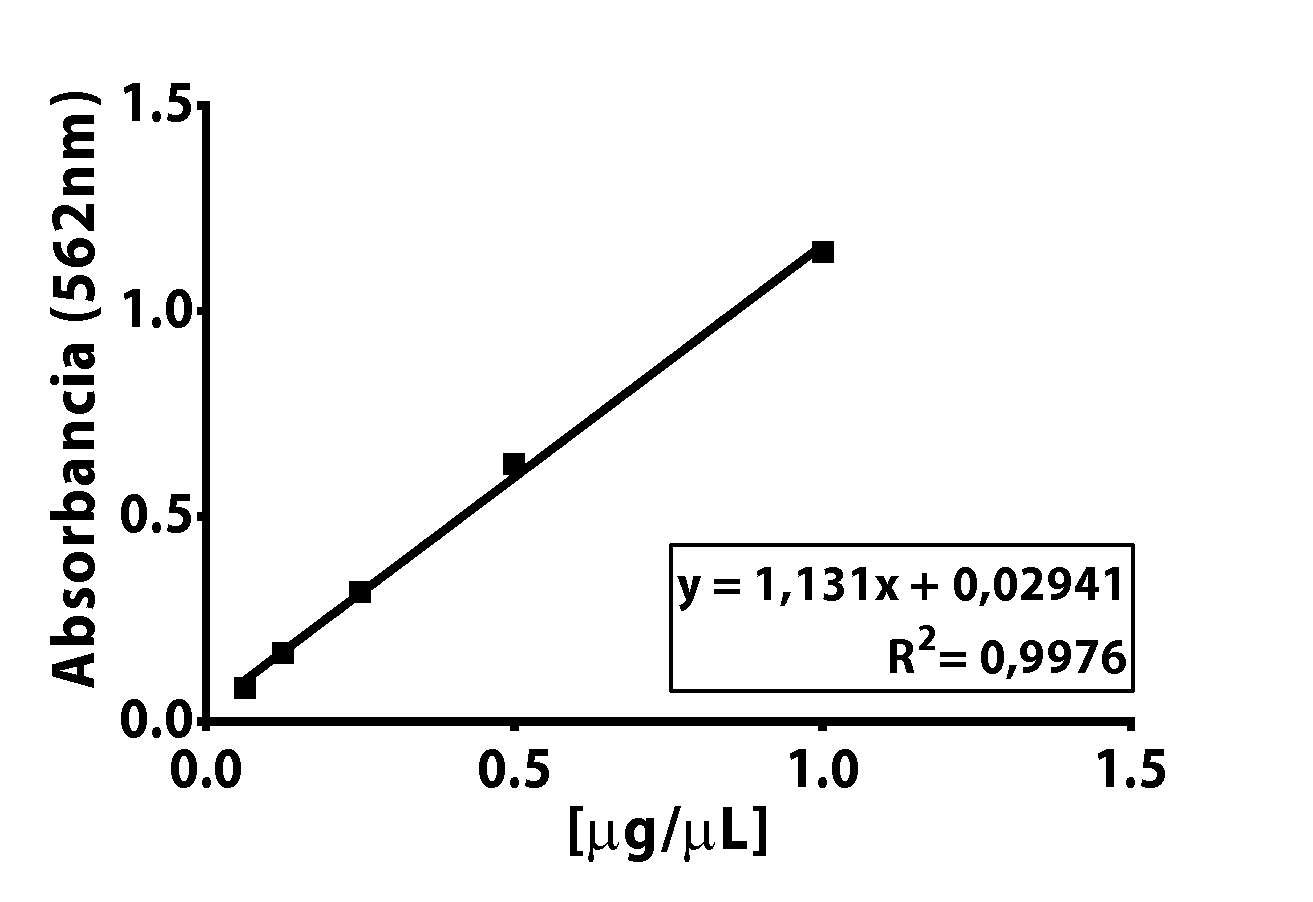
\includegraphics[width=0.4\textwidth]{BCA}
    \caption{Curva de calibrado BCA}
    \label{curvabca}
\end{figure}

\begin{displaymath}
y=1,131x+0,02941
\label{eq:BCA}
\end{displaymath}

Las cuantificaciones interpoladas en la recta de calibrado (Figura
\ref{curvabca}) se muestran en la Tabla \ref{tablaPROTEINAS}

\begin{table}[h]
\begin{center}
    \begin{threeparttable}
      \caption{Concentraciones de Proteínas totales extraídas}\label{tablaPROTEINAS}
      \begin{tabular}{l r l r l r l r l r}
    \toprule
    \textbf{ID} & \textbf{µg/µL} & \textbf{ID} & \textbf{µL/µL} & \textbf{ID} & \textbf{µL/µL} & \textbf{ID} & \textbf{µL/µL} & \textbf{ID} & \textbf{µL/µL}\\
    \midrule
    B1 & 4,14 & B21 & 3,79 & B31 & 4,10 & B41 & 3,35 & B51 & 2,70 \\
    B2 & 3,83 & B22 & 2,51 & B32 & 3,02 & B42 & 7,42 & B52 & 5,65 \\
    B3 & 3,84 & B23 & 3,20 & B33 & 9,62 & B43 & 5,20 & B53 & 4,31 \\
    B4 & 3,64 & B24 & 5,41 & B34 & 5,02 & B44 & 4,15 & B54 & 5,54 \\
    B5 & 3,66 & B25 & 6,43 & B35 & 5,88 & B45 & 6,62 & B55 & 3,18 \\
    B16 & 3,22 & B26 & 6,01 & B36 & 7,69 & B46 & 2,77 & \\
    B17 & 3,67 & B27 & 3,05 & B37 & 6,03 & B47 & 6,65 & \\
    B18 & 2,67 & B28 & 5,11 & B38 & 3,35 & B48 & 5,32 & \\
    B19 & 4,67 & B29 & 5,50 & B39 & 12,32 & B49 & 4,05 & \\
    B20 & 2,94 & B30 & 3,22 & B40 & 2,45 & B50 & 3,82 & \\
\bottomrule
\end{tabular}
\end{threeparttable}
\end{center}
\end{table}

\section{Validación de anticuerpos}

Los resultados de la validación de los anticuerpos por ELISA indirecto
fueron graficados en la Figura \ref{fig:pep}

\begin{figure}[h!]
    \begin{subfigure}{0.5\textwidth}
        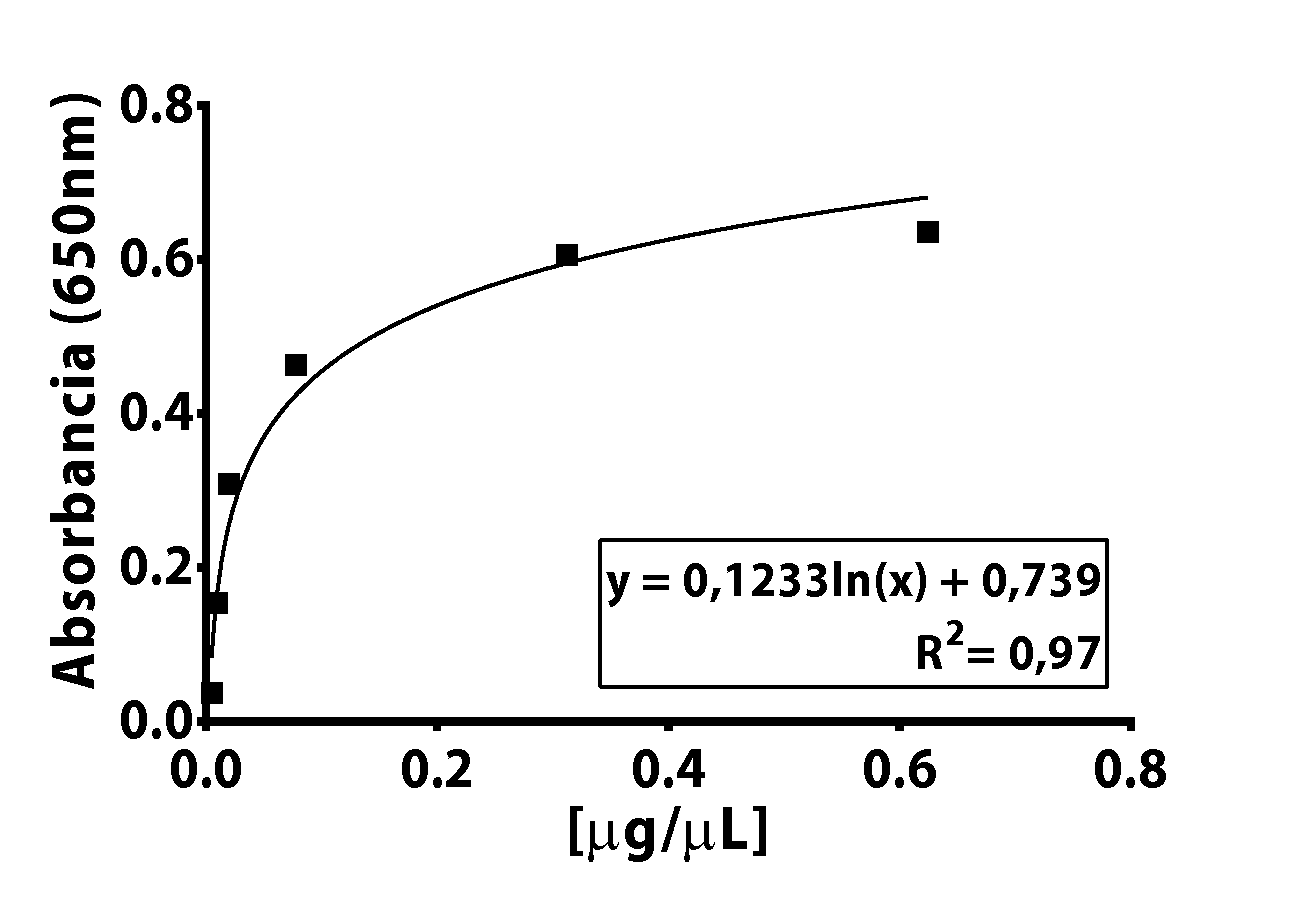
\includegraphics[width=0.9\textwidth]{peptidos/tnfa}
        \caption{TNF-$\alpha$}
        \label{fig:pep:tnfa}
        \end{subfigure}
    \begin{subfigure}{0.5\textwidth}
        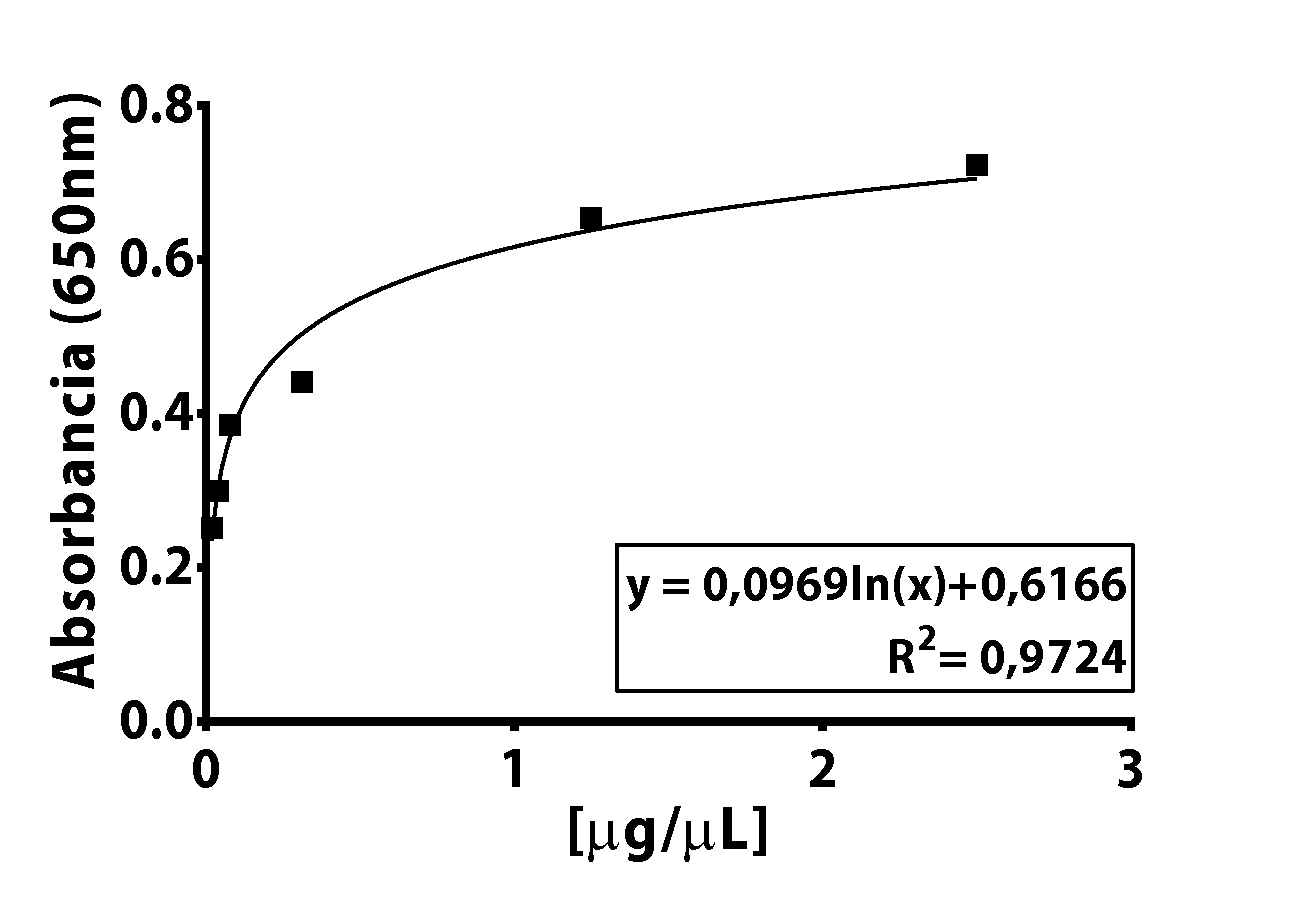
\includegraphics[width=0.9\textwidth]{peptidos/ifng}
        \caption{IFN-$\gamma$}
        \label{fig:pep:ifng}
    \end{subfigure}
      \begin{subfigure}{0.5\textwidth}
        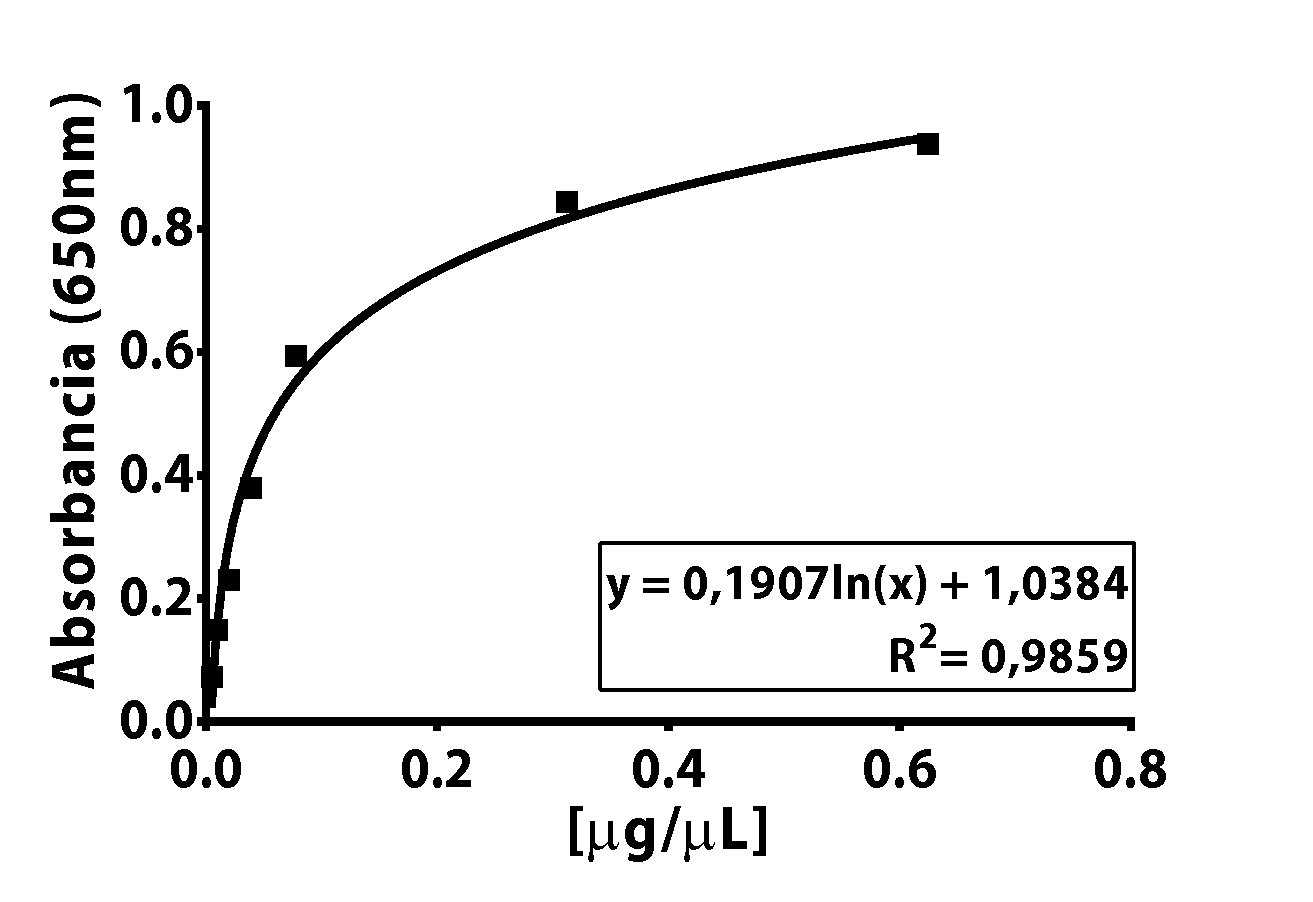
\includegraphics[width=0.9\textwidth]{peptidos/il1b}
        \caption{IL-1$\beta$}
        \label{fig:pep:il1b}
    \end{subfigure}
     \begin{subfigure}{0.5\textwidth}
        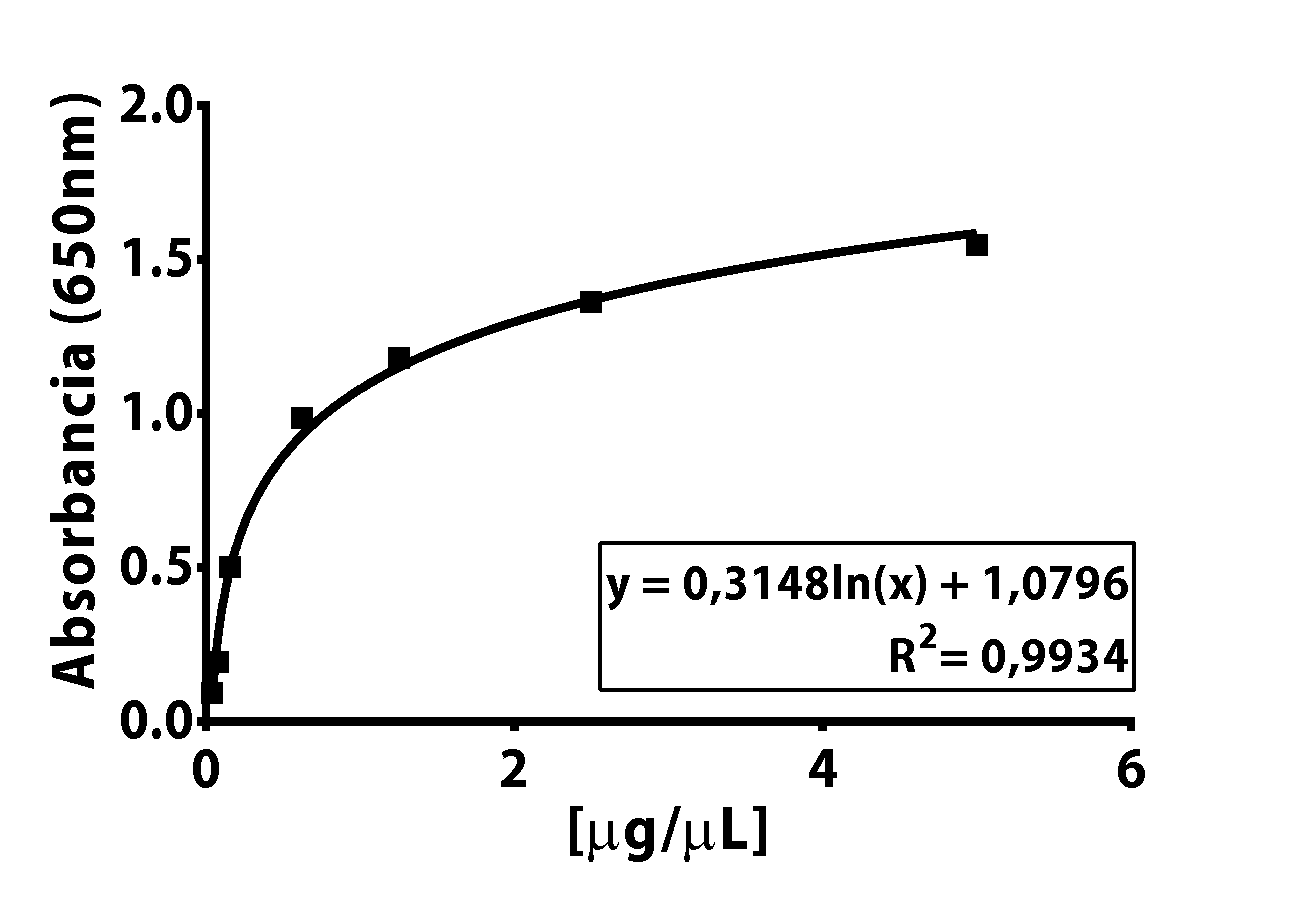
\includegraphics[width=0.9\textwidth]{peptidos/inos}
        \caption{iNOS}
        \label{fig:pep:inos}
    \end{subfigure}
    \begin{subfigure}{0.5\textwidth}
        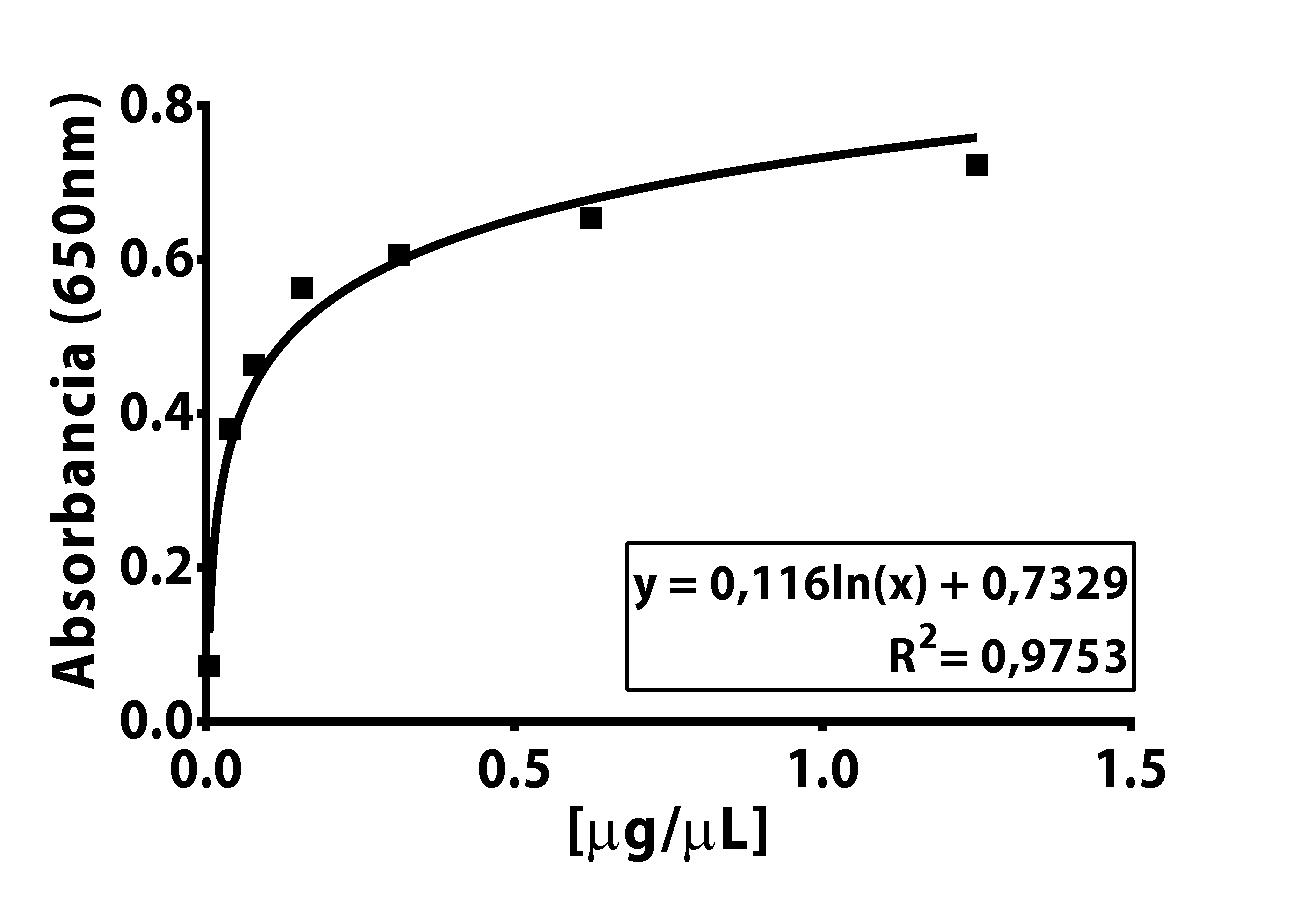
\includegraphics[width=0.9\textwidth]{peptidos/il12}
        \caption{IL-12}
        \label{fig:pep:il12}
    \end{subfigure}
    \caption{Evaluación cualitativa de los anticuerpos en estudio usando sus inmunógenos como antígenos, mediante ELISA Indirecto}
    \label{fig:pep}
\end{figure}

\subsection{Anticuerpos producidos en conejo}

Para el caso de los anticuerpos producidos en conejo,
anti-TNF-\(\alpha\) se obtuvo una curva con un \(R^2\) de 0,97 (Figura
\ref{fig:pep} \subref{fig:pep:tnfa}), el anticuerpo anti-IFN-\(\gamma\)
obtuvo una curva con un \(R^2\) de 0,9724(Figura \ref{fig:pep}
\subref{fig:pep:ifng}) y finalmente el anticuerpo anti-IL-1\(\beta\)
producido en conejo se obtuvo una curva con un \(R^2\) de 0,9859 (Figura
\ref{fig:pep} \subref{fig:pep:il1b}).

\subsection{Anticuerpos producidos en ratón}

En el caso de los anticuerpos producidos en murinos, anti-iNOS obtuvo
una curva con un \(R^2\) de 0,9934 (Figura \ref{fig:pep}
\subref{fig:pep:inos}) y para el anticuerpo anti-IL-12 se obtuvo un
\(R^2\) de 0,9753 (Figura \ref{fig:pep} \subref{fig:pep:il12}).

\section{ELISAs Indirectos}

Al evaluar mediante ELISA indirecto la disponibilidad de las distintas
moléculas en estudio en las branquias de las truchas arcoiris
alimentadas con Zimosán A, se observó una clara diferencia entre los
individuos control y los tratados (Figura \ref{fig:elisa}).

\begin{figure}[h]
    \begin{subfigure}{0.5\textwidth}
        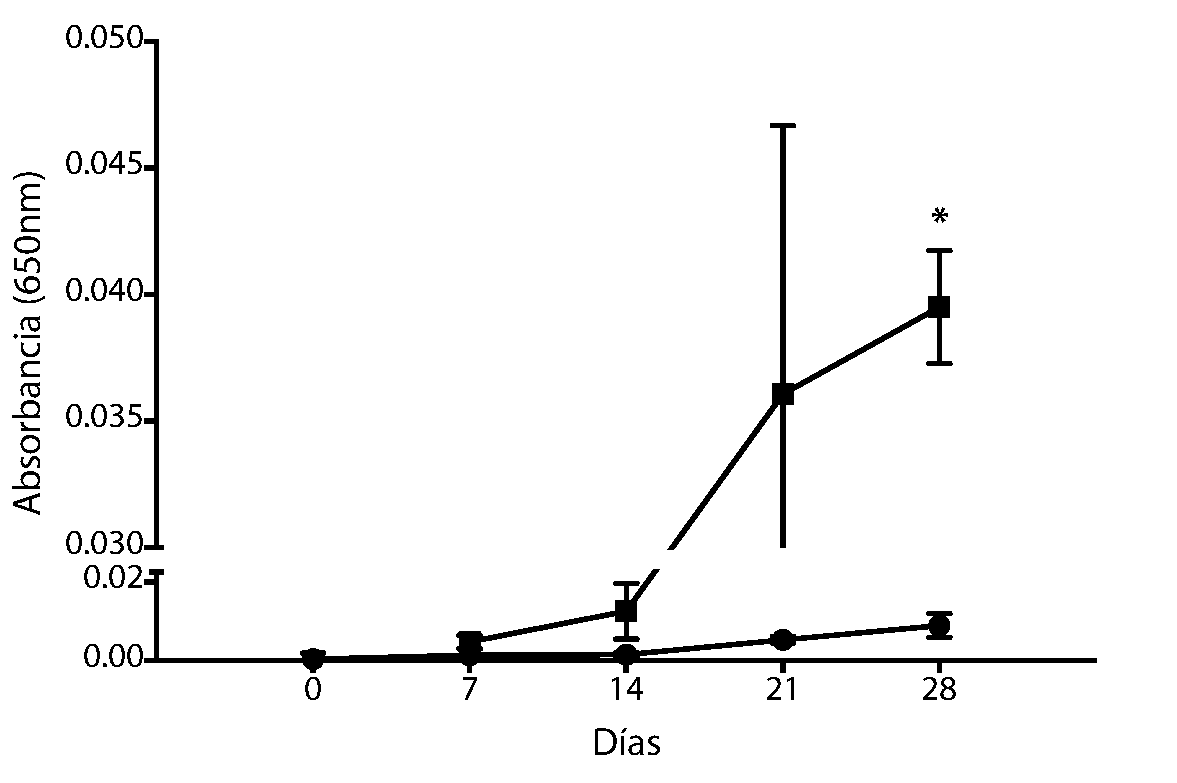
\includegraphics[width=0.9\textwidth]{eps/ELISA/pdf/etnfa}
        \caption{TNF-$\alpha$}
        \label{fig:elisa:tnfa}
        \end{subfigure}
    \begin{subfigure}{0.5\textwidth}
        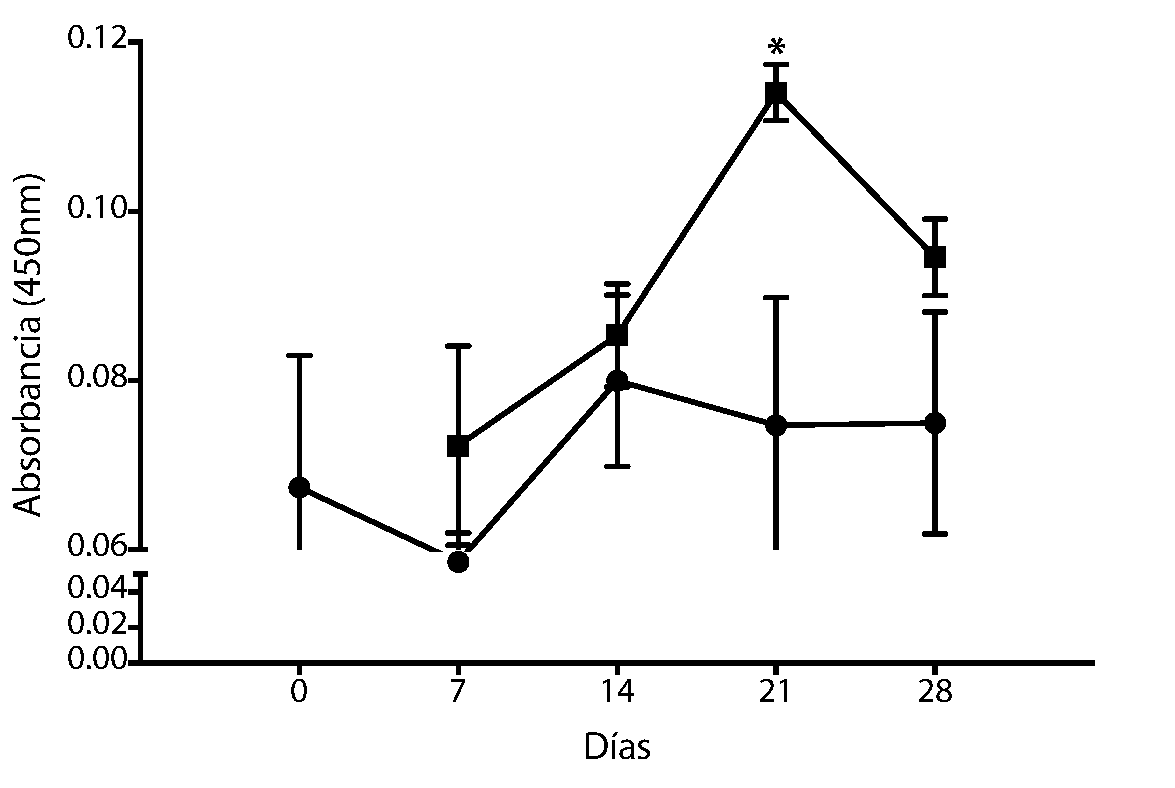
\includegraphics[width=0.9\textwidth]{eps/ELISA/pdf/eifng}
        \caption{IFN-$\gamma$}
        \label{fig:elisa:ifng}
    \end{subfigure}
    \begin{subfigure}{0.5\textwidth}
        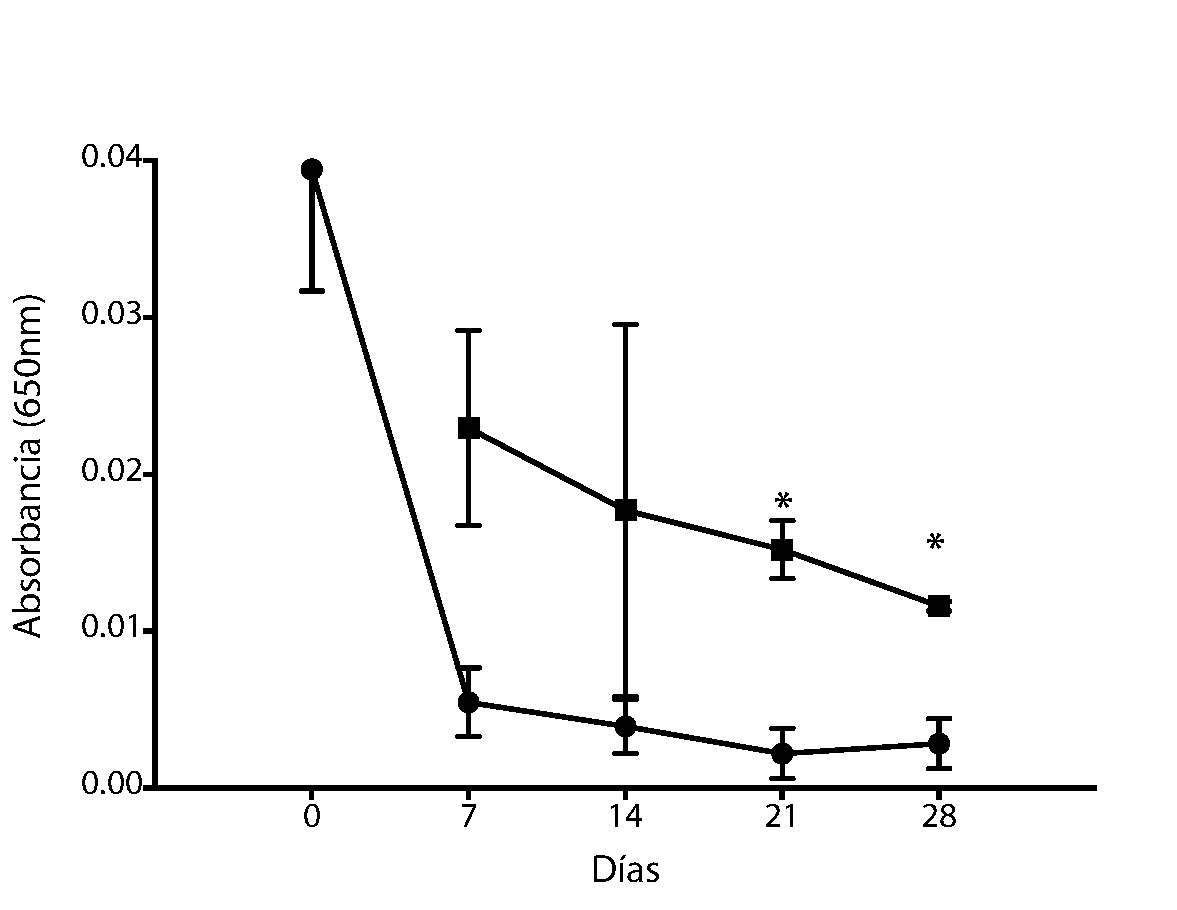
\includegraphics[width=0.9\textwidth]{eps/ELISA/pdf/eil1b}
        \caption{IL-1$\beta$}
        \label{fig:elisa:il1b}
    \end{subfigure}
    \begin{subfigure}{0.5\textwidth}
        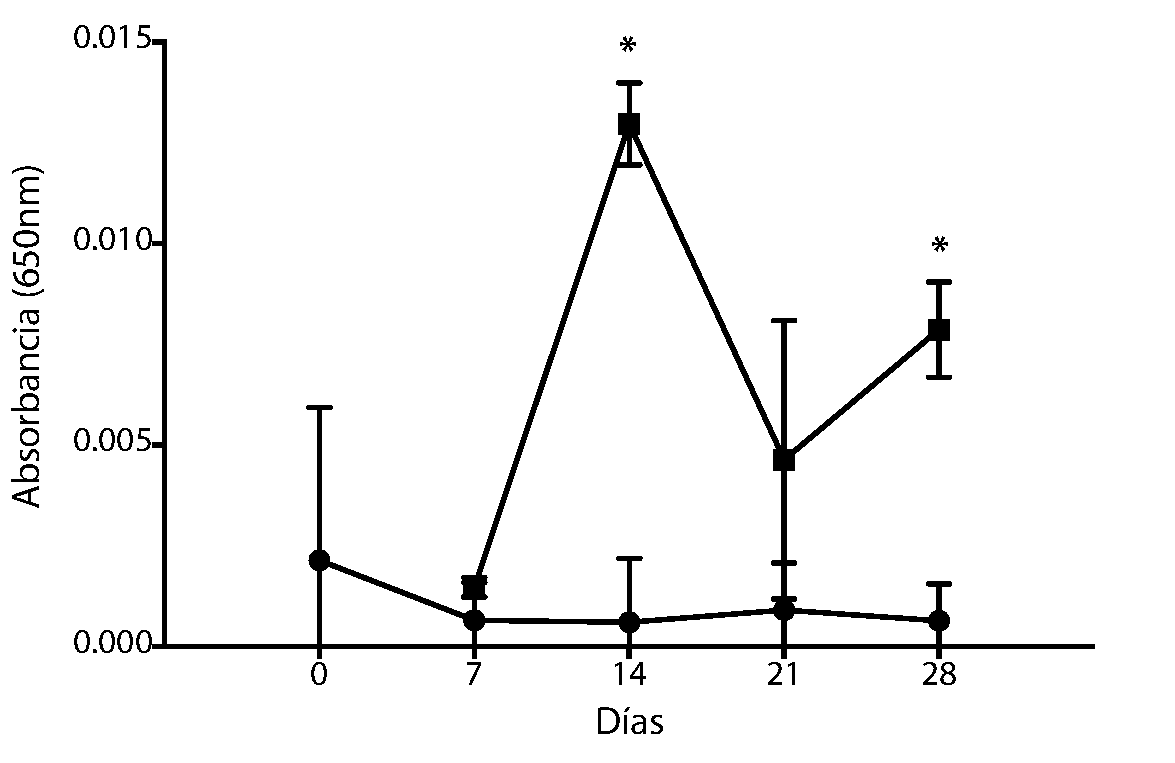
\includegraphics[width=0.9\textwidth]{eps/ELISA/pdf/einos12}
        \caption{iNOS}
        \label{fig:elisa:inos}
    \end{subfigure}
    \begin{subfigure}{0.5\textwidth}
        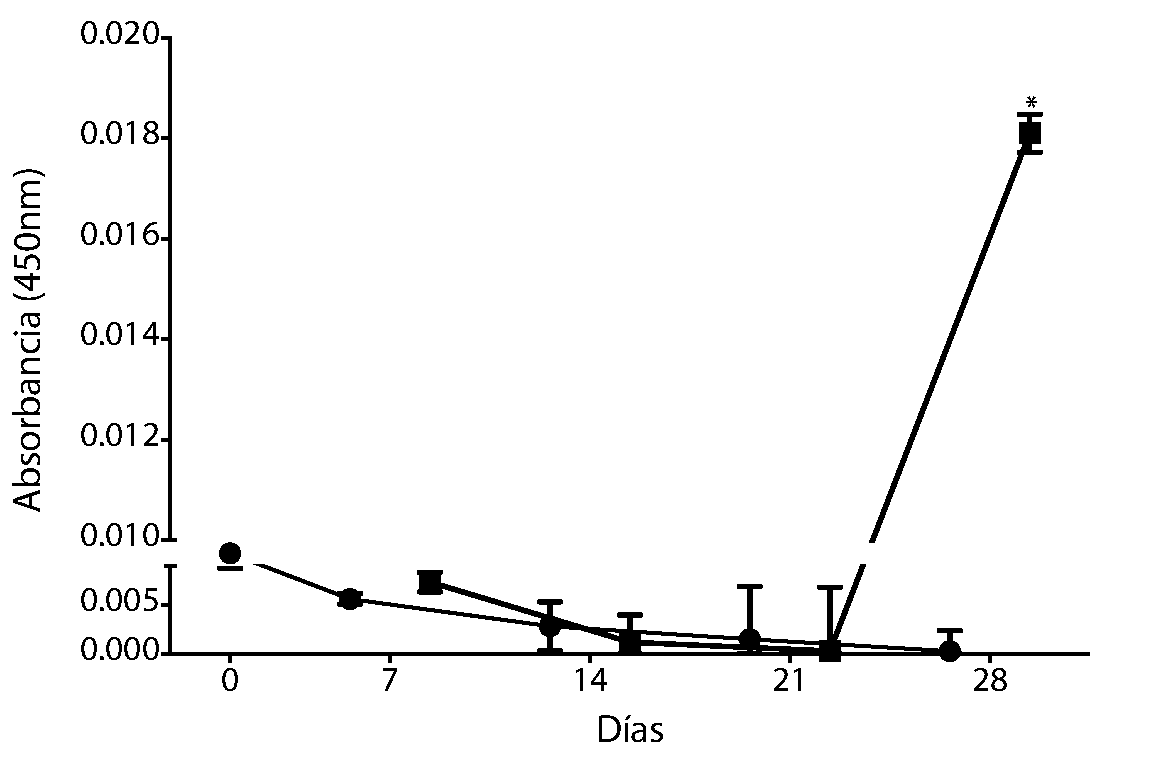
\includegraphics[width=0.9\textwidth]{eps/ELISA/pdf/eil12}
        \caption{IL-12}
        \label{fig:elisa:il12}
    \end{subfigure}
    \begin{subfigure}{0.5\textwidth}
        \includegraphics[width=0.9\textwidth]{eps/qPCR/leyenda}
    \end{subfigure}
    \caption{Detección mediante ELISA indirecto de las moléculas en estudio}
    \label{fig:elisa}
\end{figure}

\subsection{TNF-$\alpha$}

Para TNF-\(\alpha\) (Figura \ref{fig:elisa} \subref{fig:elisa:tnfa}),
respecto a su control inicial, evidenció un aumento paulatino de su
biodisponibilidad partiendo del día 7 al día 14, un aumento de
aproximadamente 4 veces el día 21 y finalmente un leve aumento el día
28, este ultimo dia siendo significativo respecto a su control
(\(p \leq 0,05\)).

\subsection{IFN-$\gamma$}

Esta molécula (Figura \ref{fig:elisa} \subref{fig:elisa:ifng}) tuvo un
leve aumento en los días 7 y 14 con respecto a su control,
evidenciandose el mayor aumento al día 21, el cual es significativo
(\(p \leq 0,05\)) con respecto a su control, para finalmente disminuir
su biodisponibilidad el día 28.

\subsection{IL-1$\beta$}

Para Interleuquina 1-\(\beta\) (Figura \ref{fig:elisa}
\subref{fig:elisa:il1b}) se observó una gran biodisponibilidad de esta
molécula en el control al inicio del tratamiento, pero esta alta
biodisponibilidad baja y se estabiliza rápidamente al día 7, en el caso
de los peces alimentados con Zimosán A se observaron desde el día 7
biodisponibilidades mayores a sus controles del día, siendo el día 21 y
28 diferentes significativamente (\(p \leq 0,05\)).

\subsection{iNOS}

Para la enzima Oxido Nítrico Sintasa inducible (Figura \ref{fig:elisa}
\subref{fig:elisa:inos}) se obtuvo el día 14 un súbito y significativo
aumento de su biodisponibilidad comparado con todo el grupo control
(\(p \leq 0,05\)), bajó el día 21 para finalmente subir paulatina y
significativamente el día 28 con respecto a su control
(\(p \leq 0,05\)).

\subsection{IL-12}

La Interleuquina 12 (Figura \ref{fig:elisa} \subref{fig:elisa:il12}) en
los peces tratados como los inducidos se obtuvo una baja en la
biodisponibilidad de esta molécula de los primeros 21 días, finalmente
después de esta medición, al día 28, hubo un aumento significativo de
aproximadamente 20 veces con respecto al control del día
(\(p \leq 0,05\)).

\subsection{Síntesis comparada del estudio}

Los anticuerpos reconocen sus respectivos epítopes (Figura
\ref{fig:pep}).

Las 5 moléculas en estudio presentaron un aumento en su disponibilidad
entre los días 21 y 28, incluso una presenta aumento el día 14.

La mayor disponibilidad de proteína se observo a nivel de IFN-\(\gamma\)
el día 21 y la menor fue para el caso de iNOS el día 28, aún así ambas
disponibilidades mayores que su control significativamente

El día con mayor disponibilidad de las proteínas en estudio fue el día
28, donde TNF-\(\alpha\), IL-1\(\beta\), iNOS e IL-12 aumentaron su
disponibilidad con respecto a sus controles sin tratamiento, mientras
que el día 21 fue el día con menor disponibilidad de las moléculas
estudiadas, en las cuales encontramos a IFN-\(\gamma\) e IL-1\(\beta\)

\clearpage

\section{Tinción Hematoxilina-eosina}

\begin{figure}[h!]
    \centering
\includegraphics[width=1\textwidth]{gills}
    \caption[Microfotografías de branquias de trucha arcoiris]{Microfotografías de branquias de trucha arcoiris con tinción Hematoxilina-eosina: A) Opérculo abierto exponiendo las branquias a extraer; B,C) Día 0; D) Día 14 Control; E) Día 14 Tratado; F) Día 21 Control; G) Día 21 Tratado; H) Día 28 Control; I) Día 28 Tratado. AB = Arco Branquial, B = Branquias, LP = Laminilla primaria, LS = Laminilla secundaria, CE = Células epiteliales CP = Células pilares}
    \label {fig:gills}
\end{figure}

Al realizar la tinción de Hematoxilina-eosina se pudo apreciar la
integridad de los distintos cortes histológicos, los tejidos que los
componen y así como también los distintos tipos celulares que se
pudieron encontrar (Figura \ref{fig:gills}). La branquia se observa
completa, sin su arco branquial, demostrando una consistencia entre sus
laminillas primarias y secundarias (Figura \ref{fig:gills} D,E), así
como también la presencia de células pilares (Figura \ref{fig:gills} C)
y células epiteliales (Figura \ref{fig:gills} F).

\section{Inmunofluorescencia}

Habiendo comprobado la integridad de los tejidos muestreados se procedió
a localizar las moléculas en estudio, usando los cortes cortes
histológicos y la técnica de inmunofluorescencia descrita en la sección
\ref{sec:ifat}, se observaron los siguientes resultados.

\subsection{TNF-$\alpha$}

Se observa un marcaje positivo en células de la laminilla secundaria las
cuales mostraban producción de TNF-\(\alpha\) (Figura
\ref{fig:gills:tnfa}).

\begin{figure}[h!]
    \centering
    \includegraphics[width=0.8\textwidth]{ifat/z/tnfa}
    \caption[Microscopía Confocal para TNF-$\alpha$]{Microscopía confocal para TNF-$\alpha$ en cortes histológicos de branquias de trucha arcoiris tratadas con Zimosán A liberado en dieta: A) Control con tinción Syto9; B) Control con tinción Alexa Fluor; C) \emph{Merge} entre ambos canales; D) Tratado con tinción Syto9; E) Tratado con tinción Alexa Fluor; F) \emph{Merge} entre ambos canales. Flechas ($\leftarrow$) = Marcaje del anticuerpo}
    \label {fig:gills:tnfa}
\end{figure}

\subsection{IFN-$\gamma$}

Se observa un marcaje positivo en células de la laminilla secundaria,
las cuales mostraban producción de interferón gamma (Figura
\ref{fig:gills:ifng}).

\begin{figure}[h!]
    \centering
    \includegraphics[width=0.8\textwidth]{ifat/z/ifng}
    \caption[Microscopía Confocal para IFN-$\gamma$]{Microscopía confocal para IFN-$\gamma$ en cortes histológicos de branquias de trucha arcoiris tratadas con Zimosán A liberado en dieta:  A) Control con tinción Syto9; B) Control con tinción Alexa Fluor; C) \emph{Merge} entre ambos canales; D) Tratado con tinción Syto9; E) Tratado con tinción Alexa Fluor; F) \emph{Merge} entre ambos canales. Flechas ($\leftarrow$) = Marcaje del anticuerpo}
    \label {fig:gills:ifng}
\end{figure}

\subsection{IL-1$\beta$}

Se observa un marcaje positivo en células de la laminilla secundaria,
las cuales mostraban producción de IL-1\(\beta\) (Figura
\ref{fig:gills:il1b}).

\begin{figure}[h!]
    \centering
    \includegraphics[width=0.8\textwidth]{ifat/z/il1b}
    \caption[Microscopía Confocal para IL-1$\beta$]{Microscopía confocal para IL-1$\beta$ en cortes histológicos de branquias de trucha arcoiris tratadas con Zimosán A liberado en dieta:  A) Control con tinción Syto9; B) Control con tinción Alexa Fluor; C) \emph{Merge} entre ambos canales; D) Tratado con tinción Syto9; E) Tratado con tinción Alexa Fluor; F) \emph{Merge} entre ambos canales. Flechas ($\leftarrow$) = Marcaje del anticuerpo}
    \label {fig:gills:il1b}
\end{figure}

\subsection{iNOS}

Se observa un marcaje positivo para la producción de iNOS en células de
la laminilla secundaria (Figura \ref{fig:gills:inos}).

\begin{figure}[h!]
    \centering
    \includegraphics[width=0.8\textwidth]{ifat/inos}
    \caption[Microscopía Confocal para iNOS]{Microscopía confocal para iNOS en cortes histológicos de branquias de trucha arcoiris tratadas con Zimosán A liberado en dieta:  A) Control con tinción Syto9; B) Control con tinción Alexa Fluor; C) \emph{Merge} entre ambos canales; D) Tratado con tinción Syto9; E) Tratado con tinción Alexa Fluor; F) \emph{Merge} entre ambos canales. Flechas ($\leftarrow$) = Marcaje del anticuerpo}
    \label {fig:gills:inos}
\end{figure}

\clearpage

\section{Correlación}

\begin{table}[h!]
\centering
\caption[Matrices de correlación de las moléculas en estudio]{Matrices de correlación de las moléculas en estudio, para qPCR y ELISA}\label{tab:corr}
\begin{subtable}{.5\textwidth}
\centering

\begin{tabular}{lrrrr}
\toprule
   & TNF-$\alpha$ & iNOS & IL-1$\beta$ & IL-12 \\ 
  \midrule
TNFa &  &  &  &  \\ 
  iNOS &  {\color{OliveGreen}0,81}  &  &  &  \\ 
  IL-1$\beta$ &  {\color{OliveGreen}0,98}  &  0,72  &  &  \\ 
  IL-12 &  {\color{OliveGreen}0,94}  &  {\color{OliveGreen}0,87}  &  {\color{OliveGreen}0,86}  &  \\ 
  IFN-$\gamma$ &  {\color{OliveGreen}0,99} &  {\color{OliveGreen}0,85}  &  {\color{OliveGreen}0,95}  &  {\color{OliveGreen}0,97}  \\ 
   \bottomrule
   \end{tabular}

\caption{qPCR}
\end{subtable}%
\begin{subtable}{.5\textwidth}
\centering

\begin{tabular}{lrrrr}
\toprule
        & TNF-$\alpha$ & iNOS & IL-1$\beta$ & IL-12 \\ 
  \midrule
  TNF-$\alpha$ & & & & \\
  iNOS &  0,31  &  &  &  \\ 
  IL-1$\beta$ & {\color{red}-0,81}  & -0,55  &  &  \\ 
  IL-12 &  0,20  & -0,15  & -0,02  &  \\ 
  IFN-$\gamma$ &  {\color{OliveGreen}0,89}  &  0,30  & -0,75  & -0,25  \\ 
   \bottomrule
   \end{tabular}

\caption{ELISA}
\end{subtable}
\end{table}

Se obtuvo una correlación muy alta (\textgreater{}0.8) para el caso de
los ensayos de qPCR (Tabla \ref{tab:corr}A), siendo la mayor correlación
positiva la dupla IFN-\(\gamma\)/TNF-\(\alpha\) con un R=0,99 y por el
contrario, la dupla con menor correlación positiva fue
IL-1\(\beta\)/iNOS.

En el caso de los ensayos de ELISA indirecto la dupla que obtuvo mayor
correlación positiva fue IFN-\(\gamma\)/TNF-\(\alpha\) con un R=0,89
mientras que para el caso de la dupla IL-1\(\beta\)/TNF-\(\alpha\) se
obtuvo una correlación negativa con un R=-0,82 (Tabla \ref{tab:corr}B).

Finalmente con el fin de saber qué marcadores se pueden usar
indistintamente del ensayo que se ocupe (en este caso qPCR y ELISA) se
correlacionaron los datos obtenidos por cada molécula en cada ensayo.

\begin{table}[h!]
\centering
\begin{threeparttable}
\caption{Correlación de Pearson para una misma molécula y distintos ensayos}\label{r.pcr}\label{tab:corrtotal}
\begin{tabularx}{10cm}{X r}
  \toprule
    Dupla   &  R \\
  \midrule
qTNF-$\alpha$/eTNF-$\alpha$ & {\color{OliveGreen}0,96} \\
qIFN-$\gamma$/eIFN-$\gamma$ & {\color{OliveGreen}0,83} \\
qIL-12/eIL-12 & 0,52 \\
qiNOS/eiNOS & 0,02 \\
qIL-1$\beta$/eIL-1$\beta$ & 0,6 \\
 \bottomrule
   \end{tabularx}
   \begin{tablenotes}
    \item q = qPCR; e = ELISA
\end{tablenotes}
\end{threeparttable}
\end{table}

Para los casos de las moléculas TNF-\(\alpha\) e IFN-\(\gamma\) se
obtuvieron correlaciones positivas \textgreater{} a 0,8 (Tabla
\ref{tab:corrtotal}). \chapter{Discusion}

La perdida del equilibrio
Ambiente\(\Leftrightarrow\)Patógeno\(\Leftrightarrow\)Hospedero es la
causa de la mayoría de las enfermedades presentes en la acuicultura, y
es por eso que es estrictamente necesario cimentar las bases de una
comprensión íntegra del sistema inmune, para así, poder generar
tecnología que pueda sobreponerse a estos paradigmas. Esto tiene suma
importancia sobretodo en la industria acuícola, la cual produce
anualmente, y con un crecimiento constante, 148 millones de toneladas de
pescado (FAO, 2012), las cuales se traducen aproximadamente en 217.500
millones de dólares (USD), mas aún, de toda esa producción, 128 millones
de toneladas fueron exclusivamente destinados a consumo humano, por lo
que las perdidas por un brote de alguna enfermedad ascienden a millones
de dólares, brotes que amenazan las año a año las operaciones acuícolas
al rededor del mundo.

Varios autores describen un aumento en la transcripción de los genes
evaluados en esta tesis, Lokesh et al (2012) observan esto en la
expresión de IFN-\(\gamma\) en \emph{G.morhua} usando una concentración
de \(\beta\)-glucano al 1\% aunque este estudio fue evaluado en
intestino. Skov et al (2012) demuestra la sobre-expresión de
IFN-\(\gamma\) de hasta 111 veces de cambio con respecto a su control
posterior a 59 días de tratamiento de inmersión con \(\beta\)-glucanos.
En el caso de la expresión de la Interleukina 1-\(\beta\) Zhang et al.
(2009) demostró en \emph{O.mykiss} que se produce una sobre expresión de
este gen a partir del dia 7 luego de tratar vía inmersión con
\(\beta\)-glucanos. En \emph{D.rerio} inyectados con \(\beta\)-glucanos
Rodriguez et al. (2009) describe una sobreexpresión de IL-1\(\beta\) de
hasta 60 veces con respecto a su control sin tratar. Finalmente, Zhang
et al (2009) demostró la sobre-expresión del gen que codifica para
TNF-\(\alpha\) luego de 14 días de inmersión con \(\beta\)-glucanos.

El primer par de partidores en estandarizar fue el de referencia, el
cual tuvo una eficiencia de 96,9\% y solo un peak en la curva de
disociación lo que nos corrobora que el primer, a 58ºC como temperatura
de annealing, genera un solo producto y que cada ciclo dobla su cantidad
inicial de templado (Figura \ref{fig:ef1a}). Para las demás parejas de
partidores correspondientes a los genes en estudio se observó la misma
tendencia, generándose eficiencias de 105,5\% para el par de partidores
que amplifican para IL-12 a 58ºC (Figura \ref{fig:il12}), 115\% para el
el par de partidores que amplifican para TNF-\(\alpha\) a 58ºC (Figura
\ref{fig:tnfa}), 120,9\% para el par de partidores que amplifican para
IFN-\(\gamma\) a 61,5ºC (Figura \ref{fig:ifng}), 105,9\% para el par de
partidores que amplifican para IL-1\(\beta\) a 58ºC (Figura
\ref{fig:il1b}) y finalmente 102\% para la pareja de partidores que
amplifican para iNOS a 58ºC (Figura \ref{fig:inos}).

Todas las eficiencias son similares, la única que se escapa levemente
del promedio es la eficiencia del par de partidores que amplifican para
IFN-\(\gamma\), esto puede deberse a que el producto o amplicón que
producen es muy pequeño (\textasciitilde{}51pb) (Tabla
\ref{tabla:partidores}) y está en el limite de lo recomendado para la
cuantificación por el método \(\Delta\Delta C_T\) (Pfaffl, 2001; Bustin
et~al., 2009).

Teniendo ya estandarizados todos los partidores se procedió a evaluar
las muestras biológicas del ensayo, en las cuales la tendencia demostró
que la respuesta inmune empieza a aumentar pasado el día 14, ya que
todos los peak de expresión se observaron en los días 21 y 28 según
corresponda. (Figura \ref{fig:qpcr}), esto se corrobora con varios
estudios donde los tiempos de respuesta frente a \(\beta\)-glucanos en
tratamientos \emph{in vivo} rondan dentro o después de los 21 días
(Casadei et~al., 2012; Skov et~al., 2012; Dobšíková et~al., 2013).

Para el caso de varios controles en distintas moléculas también se
observo un aumento pasado este día, esto puede deberse a un estrés en
los peces, el cual haya gatillado un aumento en la respuesta inmune como
se ha demostrado en estudios anteriores (Bricknell y Dalmo, 2005;
Magnadóttir, 2006; Barandica y Tort, 2008; Bowden, 2008), pero aún
teniendo controles altos en los ensayos de transcripción, por ejemplo
para TNF-\(\alpha\) (Figura \ref{fig:qpcr}A), IFN-\(\gamma\) (Figura
\ref{fig:qpcr}B) e IL-1\(\beta\) (Figura \ref{fig:qpcr}C) estas
diferencias entre tratamientos siguen siendo estadísticamente
significativas (\(p < 0,05\)).

Teniendo estos datos en cuenta se puede deducir que el suplementar la
alimentación de los peces con \emph{Zimosán A} liberado en dieta
promovería la expresión de los genes que codifican para distintas
citoquinas pro-inflamatorias y moléculas efectoras de inmunidad.

Para los 5 anticuerpos usados en el estudio se obtuvieron curvas
logarítmicas con un coeficiente \(R^2 > 0,97\), esto significa que a
mayor concentración de inmunógeno (péptido sintético) el anticuerpo se
va saturando, mientras que al inicio de la curva hay una linealidad en
la reacción. Con estos resultados se aprobó el uso de estos anticuerpos
en ensayos de ELISA indirectos con muestra biológica como antígeno.

Todas las moléculas en estudio aumentaron su biodisponibilidad con
respecto a sus controles, observando una tendencia similar a lo
demostrado por Morales-Lange et al (2014) en su estudio usando el
\(\beta\)-glucano Laminarín. Chansue et al (2000). demostró en tilapia
la disponibilidad luego del día 5 de tratamiento de TNF-\(\alpha\)
usando \(\beta\)-glucanos en una concentración al 2\% entregados por vía
oral. Tomando en cuenta el dogma de la biología molecular debiese haber
obtenido los peak de biodisponibilidad de Proteínas posteriormente a los
de transcrito, y hubieron casos, en que hubo peaks al mismo día que en
lo visto por PCR en tiempo real(Figuras \ref{fig:elisa} y
\ref{fig:qpcr}). Esto se puede deber a que exista un intervalo de tiempo
anterior al medido en que se pueda apreciar la diferencia entre ambas
condiciones y la biodisponibilidad de proteínas que estamos observando
corresponde a una traducción de transcrito de algún día anterior no
evaluado, y finalmente, otra razón de este fenómeno sería la documentada
presencia de leucocitos circulantes en las branquias (Castro et~al.,
2014) los cuales estarían produciendo estas distintas moléculas
reguladoras y efectoras de inmunidad.

Cabe destacar que la baja absorbancia obtenida en los ensayos se debe a
que el efecto del \emph{Zimosán A} a esa concentración produce solo un
leve aumento en la respuesta inmune, lo cual está diseñado de esa forma,
ya que en este estudio tampoco se esperaba un estallido inflamatorio a
nivel sistémico en el pez.

Sin embargo, a pesar de lo anteriormente mencionado, en los muestreos
posteriores al día 14 se aprecia un aumento sostenido en la
biodisponibilidad de todas las moléculas, con diferencias significativas
frente a sus controles, lo que corrobora lo visto a nivel de transcrito,
la liberación de Zimosán A en dieta genera una respuesta inmune
detectable a nivel de mRNA y proteínas.

Los resultados planteados en esta tesis sentarían las bases para
plantear que el receptor de \(\beta\)-glucanos descrito para
\emph{Salmo salar} (Guselle et~al., 2006; Morales-Lange et~al., 2014)
podría estar conservado dentro de la familia de los salmónidos.
\chapter{Conclusiones}

Los análisis desarrollados en esta tesis demuestran que al tratar a
\emph{O.mykiss} con \emph{Zimosan A} liberado en dieta, hay una
respuesta inmune en su tejido branquial, detectable y cuantificable a
nivel de transcrito y proteína, lo cual permite generar un modelo
molecular preliminar asociado a estos eventos (Figura \ref{fig:modelo}),
por lo cual se da por aceptada la hipótesis planteada en este trabajo.

Sintetizando:

\begin{itemize}
\item Se observa una respuesta inmune en tejido branquial de \emph{O.mykiss} al ser tratados con \emph{Zimosán A} liberado en dieta.
\item Esta respuesta es cuantificable y detectable a nivel de transcrito y proteínas.
\item Usando una concentración de 0,3\% de \emph{Zimosán A} esta respuesta puede ser detectada desde el día 21 de su tratamiento
\item Si bien los 5 marcadores propuestos en este ensayo, se sugiere utilizar específicamente (por su coeficiente de correlación de Pearson) TNF-$\alpha$ e IFN-$\gamma$, ya sea a nivel de transcrito o proteína
\item Los anticuerpos policlonales mono-específicos producidos por el Grupo de Marcadores Inmunológicos en Organismos Acuáticos del GIM-PUCV son una alternativa viable y económica para medir estos marcadores usando una pequeña cantidad de tejido.
\end{itemize}

El aumento de moléculas efectoras y reguladoras de inmunidad deben dotar
al pez de una mejor respuesta inmune frente a los distintos patógenos a
los que podrían estar enfrentados en el cultivo de esta especie.

Este trabajo sienta las bases concretas para que futuras investigaciones
se puedan centrar en el uso de \(\beta\)-glucanos, en especial
\emph{Zimosán A}, como inmunoestimulantes en distintas etapas de
crecimiento del pez, así como también la prueba de distintas
concentraciones y vías de liberación de estos compuestos.

\begin{figure}[h!]
\centering
    \includegraphics[width=0.8\textwidth]{modelo}
    \caption[Modelo molecular propuesto de respuesta inmune]{\textbf{Modelo molecular propuesto de respuesta inmune:} Generado a partir de los resultados obtenidos en tejido branquial de truchas arcoiris tratadas con \emph{Zimosán A} liberado en dieta, inmunoestimulante que llegaría a su receptor (¿$\beta$-glucano?, ¿Dectin-1 \emph{like}?), el cual generaría la cascada de señalización para promover una respuesta inmune sintetizando citoquinas como TNF-$\alpha$, IL-1$\beta$, IL-12 e IFN-$\gamma$ y a su vez promover un ambiente oxidativo con la síntesis de iNOS en células tipo NK}
    \label{fig:modelo}
\end{figure}

\chapter{Bibliografía}

Abarca, A. (2011). \emph{Implementación de un modelo in vitro para
determinar el poder inmunoestimulante de b-glucanos en macrofagos de
trucha arcoiris} (PhD thesis). Pontificia Universidad Catolica de
Valparaiso.

Abarca, A., Bethke, J., Narváez, E., Flores, R., \& Mercado, L. (2012).
Parameters to evaluate the immunostimulant effect of Zymosan A in head
kidney leucocytes ( HKL ) of salmonids Parámetros para la evaluación del
efecto de Zimosán A como inmunoestimulante sobre leucocitos de riñón
cefálico ( HKL ) de salmónidos, \emph{40}(3), 545-552.

Aghaallaei, N., Bajoghli, B., Schwarz, H., Schorpp, M., \& Boehm, T.
(2010). Characterization of mononuclear phagocytic cells in medaka fish
transgenic for a cxcr3a:gfp reporter. \emph{Proceedings of the National
Academy of Sciences of the United States of America}, \emph{107}(42),
18079-84.

Ai, Q., Mai, K., Zhang, L., Tan, B., Zhang, W., Xu, W., \& Li, H.
(2007). Effects of dietary beta-1, 3 glucan on innate immune response of
large yellow croaker, Pseudosciaena crocea. \emph{Fish \& shellfish
immunology}, \emph{22}(4), 394-402.

Akramiene, D., Kondrotas, A., Didziapetriene, J., \& Kevelaitis, E.
(2007). Effects of beta-glucans on the immune system. \emph{Medicina
(Kaunas, Lithuania)}, \emph{43}(8), 597-606.

Alvarez-Pellitero, P. (2008). Fish immunity and parasite infections:
from innate immunity to immunoprophylactic prospects. \emph{Veterinary
immunology and immunopathology}, \emph{126}(3-4), 171-98.

Athanasopoulou, S., Marioli, D., Mikrou, A., Papanastasiou, A. D., \&
Zarkadis, I. K. (2009). Cloning and characterization of the trout
perforin. \emph{Fish \& shellfish immunology}, \emph{26}(6), 908-12.

Athman, R., \& Philpott, D. (2004). Innate immunity via Toll-like
receptors and Nod proteins. \emph{Current opinion in microbiology},
\emph{7}(1), 25-32.

Bagni, M., Romano, N., Finoia, M. G., Abelli, L., Scapigliati, G.,
Tiscar, P. G., \ldots{} Marino, G. (2005). Short- and long-term effects
of a dietary yeast beta-glucan (Macrogard) and alginic acid (Ergosan)
preparation on immune response in sea bass (Dicentrarchus labrax).
\emph{Fish \& shellfish immunology}, \emph{18}(4), 311-25.

Barandica, L., \& Tort, L. (2008). Neuroendocrinología e inmunologia de
la respuesta al estres en peces. \emph{Revista de la Academia Colombiana
de Ciencias Exactas, Físicas y Naturales}, \emph{32}(123), 267-284.

Bei, J.-X., Suetake, H., Araki, K., Kikuchi, K., Yoshiura, Y., Lin,
H.-R., \& Suzuki, Y. (2006). Two interleukin (IL)-15 homologues in fish
from two distinct origins. \emph{Molecular immunology}, \emph{43}(7),
860-9.

Bengtén, E., Quiniou, S. M.-A., Stuge, T. B., Katagiri, T., Miller, N.
W., Clem, L. W., \ldots{} Wilson, M. (2002). The IgH Locus of the
Channel Catfish, Ictalurus punctatus, Contains Multiple Constant Region
Gene Sequences: Different Genes Encode Heavy Chains of Membrane and
Secreted IgD. \emph{The Journal of Immunology}, \emph{169}(5),
2488-2497.

Bethke, J., Rojas, V., Berendsen, J., Cárdenas, C., Guzmán, F.,
Gallardo, J. a, \& Mercado, L. (2012). Development of a new antibody for
detecting natural killer enhancing factor (NKEF)-like protein in
infected salmonids. \emph{Journal of fish diseases}, \emph{35}(5),
379-88.

Bilen, S., Bulut, M., \& Bilen, A. M. (2011). Immunostimulant effects of
Cotinus coggyria on rainbow trout (Oncorhynchus mykiss). \emph{Fish \&
shellfish immunology}, \emph{30}(2), 451-5.

Bird, S., Zou, J., Kono, T., Sakai, M., Dijkstra, J. M., \& Secombes, C.
(2005a). Characterisation and expression analysis of interleukin 2
(IL-2) and IL-21 homologues in the Japanese pufferfish, Fugu rubripes,
following their discovery by synteny. \emph{Immunogenetics},
\emph{56}(12), 909-23.

Bird, S., Zou, J., Savan, R., Kono, T., Sakai, M., Woo, J., \& Secombes,
C. (2005b). Characterisation and expression analysis of an interleukin 6
homologue in the Japanese pufferfish, Fugu rubripes. \emph{Developmental
and comparative immunology}, \emph{29}(9), 775-89.

Boehm, U., Klamp, T., Groot, M., \& Howard, J. C. (1997). Cellular
responses to interferon-gamma. \emph{Annual review of immunology},
\emph{15}, 749-95.

Bogdan, C. (2001). Nitric oxide and the immune response. \emph{Nature
immunology}, \emph{2}(10), 907-16.

Boltaña, S., Roher, N., Goetz, F. W., \& Mackenzie, S. A. (2011). PAMPs,
PRRs and the genomics of gram negative bacterial recognition in fish.
\emph{Developmental and comparative immunology}, \emph{35}(12),
1195-203.

Boschi, I., Randelli, E., Buonocore, F., Casani, D., Bernini, C.,
Fausto, a M., \& Scapigliati, G. (2011). Transcription of T cell-related
genes in teleost fish, and the European sea bass (Dicentrarchus labrax)
as a model. \emph{Fish \& shellfish immunology}, \emph{31}(5), 655-62.

Boshra, H., Li, J., Peters, R., Hansen, J., Matlapudi, A., \& Sunyer, J.
O. (2004). Cloning, expression, cellular distribution, and role in
chemotaxis of a C5a receptor in rainbow trout: the first identification
of a C5a receptor in a nonmammalian species. \emph{Journal of immunology
(Baltimore, Md. : 1950)}, \emph{172}(7), 4381-90.

Bowden, T. J. (2008). Modulation of the immune system of fish by their
environment. \emph{Fish \& shellfish immunology}, \emph{25}(4), 373-83.

Bricknell, I., \& Dalmo, R. a. (2005). The use of immunostimulants in
fish larval aquaculture. \emph{Fish \& shellfish immunology},
\emph{19}(5), 457-72.

Brown, G. D., \& Gordon, S. (2001). Immune recognition. A new receptor
for beta-glucans. \emph{Nature}, \emph{413}(6851), 36-7.

Bustin, S. a, Benes, V., Garson, J. a, Hellemans, J., Huggett, J.,
Kubista, M., \ldots{} Wittwer, C. T. (2009). The MIQE guidelines:
minimum information for publication of quantitative real-time PCR
experiments. \emph{Clinical chemistry}, \emph{55}(4), 611-22.

Casadei, E., Bird, S., González, J. L., Wadsworth, S., \& Secombes, C.
J. (2012). Fish \& Shell fi sh Immunology The effect of peptidoglycan
enriched diets on antimicrobial peptide gene expression in rainbow trout
( Oncorhynchus mykiss ). \emph{Fish and Shellfish Immunology},
(December), 1-9.

Castro, R., Bernard, D., Lefranc, M. P., Six, a, Benmansour, a, \&
Boudinot, P. (2011). T cell diversity and TcR repertoires in teleost
fish. \emph{Fish \& shellfish immunology}, \emph{31}(5), 644-54.

Castro, R., Bromage, E., Abós, B., Pignatelli, J., {González Granja},
A., Luque, A., \& Tafalla, C. (2014). CCR7 is mainly expressed in
teleost gills, where it defines an IgD+IgM- B lymphocyte subset.
\emph{Journal of immunology (Baltimore, Md. : 1950)}, \emph{192}(3),
1257-66.

Chang, M., Collet, B., Nie, P., Lester, K., Campbell, S., Secombes, C.
J., \& Zou, J. (2011). Expression and functional characterization of the
RIG-I-like receptors MDA5 and LGP2 in Rainbow trout (Oncorhynchus
mykiss). \emph{Journal of virology}, \emph{85}(16), 8403-12.

Chansue, N., Endo, M., Kono, T., \& Sakai, M. (2000). The Stimulation of
Cytokine-like Proteins in Tilapia ( Oreochromis niloticus ) Orally
Treated, \emph{13}, 271-278.

Chettri, J. K., Kania, P. W., \& Buchmann, K. (2013). Immunomodulation
of rainbow trout ( Oncorhynchus mykiss ) fry by bath exposure to a
\(\beta\)-glucan from Euglena gracilis. \emph{Aquaculture Research},
\emph{44}(9), 1407-1415.

Dalmo, R. a, \& Bøgwald, J. (2008). Beta-glucans as conductors of immune
symphonies. \emph{Fish \& shellfish immunology}, \emph{25}(4), 384-96.

Dobšíková, R., Blahová, J., Mikulíková, I., Modrá, H., Prášková, E.,
Svobodová, Z., \ldots{} Siwicki, A.-K. (2013). The effect of oyster
mushroom \(\beta\)-1.3/1.6-D-glucan and oxytetracycline antibiotic on
biometrical, haematological, biochemical, and immunological indices, and
histopathological changes in common carp (Cyprinus carpio L.).
\emph{Fish \& shellfish immunology}, \emph{35}(6), 1813-23.

Engstad, R. E., \& Robertsen, B. (1994). Specificity of a beta-glucan
receptor on macrophages from Atlantic salmon (Salmo salar L.).
\emph{Developmental and comparative immunology}, \emph{18}(5), 397-408.

Falco, A., Frost, P., Miest, J., Pionnier, N., Irnazarow, I., \& Hoole,
D. (2012). Reduced inflammatory response to Aeromonas salmonicida
infection in common carp (Cyprinus carpio L.) fed with \(\beta\)-glucan
supplements. \emph{Fish \& shellfish immunology}, \emph{32}(6), 1051-7.

Falco, A., Miest, J. J., Pionnier, N., Pietretti, D., Forlenza, M.,
Wiegertjes, G. F., \& Hoole, D. (2014). \(\beta\)-Glucan-supplemented
diets increase poly(I:C)-induced gene expression of Mx, possibly via
Tlr3-mediated recognition mechanism in common carp (Cyprinus carpio).
\emph{Fish \& shellfish immunology}, \emph{36}(2), 494-502.

FAO. (2012). \emph{El estado mundial de la pesca y la acuicultura -
2012} (p. 251).

Fernández, A., Ruiz, I., \& Blas, I. D. (2002). El sistema inmune de los
teleósteos (I): Células y órganos. \emph{Revista AquaTIC}, \emph{16}.

Fields, B. N., Knipe, D. M., \& Howley, P. M. (2007). \emph{Fields'
Virology}. Wolters Kluwer Health/Lippincott Williams \& Wilkins.

Fischer, U., Koppang, E. O., \& Nakanishi, T. (2013). Teleost T and NK
cell immunity. \emph{Fish \& shellfish immunology}, \emph{35}(2),
197-206.

Fornshell, G. (2002). Rainbow Trout --- Challenges and Solutions.
\emph{Reviews in Fisheries Science}, \emph{10}(3-4), 545-557.

Georgiadis, M., Gardner, I., \& Hedrick, R. (2001). The role of
epidemiology in the prevention, diagnosis, and control of infectious
diseases of fish. \emph{Preventive Veterinary Medicine}, \emph{48}(4),
287-302.

Gomez, D., Sunyer, J. O., \& Salinas, I. (2013). The mucosal immune
system of fish: the evolution of tolerating commensals while fighting
pathogens. \emph{Fish \& shellfish immunology}, \emph{35}(6), 1729-39.

Gordon, S. (2002). Pattern recognition receptors: doubling up for the
innate immune response. \emph{Cell}, \emph{111}(7), 927-30.

Groot, C., \& Margolis, L. (1991). \emph{Pacific Salmon Life Histories}.
University of British Columbia Press.

Gunimaladevi, I., Savan, R., \& Sakai, M. (2006). Identification,
cloning and characterization of interleukin-17 and its family from
zebrafish. \emph{Fish \& shellfish immunology}, \emph{21}(4), 393-403.

Guselle, N. J., Markham, R. J. F., \& Speare, D. J. (2006). Short
communication to rainbow trout , Oncorhynchus mykiss ( Walbaum ),
protects against Loma salmonae, 375-381.

Hong, S., Zou, J., Collet, B., Bols, N. C., \& Secombes, C. J. (2004).
Analysis and characterisation of IL-1beta processing in rainbow trout,
Oncorhynchus mykiss. \emph{Fish \& shellfish immunology}, \emph{16}(3),
453-9.

Huising, M. O., Meulen, T. van der, Flik, G., \& {Verburg-van Kemenade},
B. M. L. (2004). Three novel carp CXC chemokines are expressed early in
ontogeny and at nonimmune sites. \emph{European journal of biochemistry
/ FEBS}, \emph{271}(20), 4094-106.

Huising, M. O., Schijndel, J. E. van, Kruiswijk, C. P., Nabuurs, S. B.,
Savelkoul, H. F. J., Flik, G., \& {Verburg-van Kemenade}, B. M. L.
(2006). The presence of multiple and differentially regulated
interleukin-12p40 genes in bony fishes signifies an expansion of the
vertebrate heterodimeric cytokine family. \emph{Molecular immunology},
\emph{43}(10), 1519-33.

Jault, C., Pichon, L., \& Chluba, J. (2004). Toll-like receptor gene
family and TIR-domain adapters in Danio rerio. \emph{Molecular
immunology}, \emph{40}(11), 759-71.

Kawai, T., \& Akira, S. (2005). Pathogen recognition with Toll-like
receptors. \emph{Current opinion in immunology}, \emph{17}(4), 338-44.

Kawai, T., \& Akira, S. (2010). The role of pattern-recognition
receptors in innate immunity: update on Toll-like receptors.
\emph{Nature immunology}, \emph{11}(5), 373-84.

Kono, T., Bird, S., Sonoda, K., Savan, R., Secombes, C. J., \& Sakai, M.
(2008). Characterization and expression analysis of an interleukin-7
homologue in the Japanese pufferfish, Takifugu rubripes. \emph{The FEBS
journal}, \emph{275}(6), 1213-26.

Kumari, J., \& Sahoo, P. K. (2006). Dietary immunostimulants influence
specific immune response and resistance of healthy and immunocompromised
Asian catfish Clarias batrachus to Aeromonas hydrophila infection.
\emph{Diseases of aquatic organisms}, \emph{70}(1-2), 63-70.

Kühlwein, H., Merrifield, D. L., Rawling, M. D., Foey, a D., \& Davies,
S. J. (2014). Effects of dietary \(\beta\)-(1,3)(1,6)-D-glucan
supplementation on growth performance, intestinal morphology and
haemato-immunological profile of mirror carp (Cyprinus carpio L.).
\emph{Journal of animal physiology and animal nutrition}, \emph{98}(2),
279-89.

Lazado, C. C., \& Caipang, C. M. A. (2014). Mucosal immunity and
probiotics in fish. \emph{Fish \& shellfish immunology}, \emph{39}(1),
78-89.

Lee, M. S., \& Kim, Y.-J. (2007). Signaling pathways downstream of
pattern-recognition receptors and their cross talk. \emph{Annual review
of biochemistry}, \emph{76}, 447-80.

Li, J.-H., Shao, J.-Z., Xiang, L.-X., \& Wen, Y. (2007). Cloning,
characterization and expression analysis of pufferfish interleukin-4
cDNA: the first evidence of Th2-type cytokine in fish. \emph{Molecular
immunology}, \emph{44}(8), 2078-86.

Lin, S., Pan, Y., Luo, L., \& Luo, L. (2011). Effects of dietary
\(\beta\)-1,3-glucan, chitosan or raffinose on the growth, innate
immunity and resistance of koi (Cyprinus carpio koi). \emph{Fish \&
shellfish immunology}, \emph{31}(6), 788-94.

Lokesh, J., Fernandes, J. M. O., Korsnes, K., Bergh, O., Brinchmann, M.
F., \& Kiron, V. (2012). Transcriptional regulation of cytokines in the
intestine of Atlantic cod fed yeast derived mannan oligosaccharide or
\(\beta\)-glucan and challenged with Vibrio anguillarum. \emph{Fish \&
shellfish immunology}, \emph{33}(3), 626-31.

Lucas, J. S., \& Southgate, P. C. (2012). \emph{Aquaculture: Farming
Aquatic Animals and Plants} (2.ª ed.). Wiley-Blackwell.

Løvoll, M., Fischer, U., Mathisen, G. S., Bøgwald, J., Ototake, M., \&
Dalmo, R. a. (2007). The C3 subtypes are differentially regulated after
immunostimulation in rainbow trout, but head kidney macrophages do not
contribute to C3 transcription. \emph{Veterinary immunology and
immunopathology}, \emph{117}(3-4), 284-95.

MacMicking, J., Xie, Q. W., \& Nathan, C. (1997). Nitric oxide and
macrophage function. \emph{Annual review of immunology}, \emph{15},
323-50.

Magnadóttir, B. (2006). Innate immunity of fish (overview). \emph{Fish
\& shellfish immunology}, \emph{20}(2), 137-51.

Medzhitov, R., \& Janeway, C. A. (2000). How does the immune system
distinguish self from nonself? \emph{Seminars in immunology},
\emph{12}(3), 185-8; discussion 257-344.

Misra, C. K., Das, B. K., Mukherjee, S. C., \& Pattnaik, P. (2006).
Effect of multiple injections of beta-glucan on non-specific immune
response and disease resistance in Labeo rohita fingerlings. \emph{Fish
\& shellfish immunology}, \emph{20}(3), 305-19.

Morales-Lange, B., Bethke, J., Schmitt, P., \& Mercado, L. (2014).
Phenotypical parameters as a tool to evaluate the immunostimulatory
effects of laminarin in Oncorhynchus mykiss. \emph{Aquaculture
Research}, n/a-n/a.

Mulero, I., {Pilar Sepulcre}, M., Roca, F. J., Meseguer, J.,
García-Ayala, A., \& Mulero, V. (2008). Characterization of macrophages
from the bony fish gilthead seabream using an antibody against the
macrophage colony-stimulating factor receptor. \emph{Developmental and
comparative immunology}, \emph{32}(10), 1151-9.

Narváez, E., Berendsen, J., Guzmán, F., Gallardo, J. a, \& Mercado, L.
(2010). An immunological method for quantifying antibacterial activity
in Salmo salar (Linnaeus, 1758) skin mucus. \emph{Fish \& shellfish
immunology}, \emph{28}(1), 235-9.

Oikawa, B. Y. S., \& Itazawa, Y. (1985). Gill and Body Surface Areas of
the Carp in relation to Body Mass, With Special Reference To The
Metabolism-Size Relationship. \emph{The Journal of experimental
biology}, \emph{14}(117), 1-14.

Olabuenaga, S. E. (2000). Sistema inmune en peces. \emph{Gayana
(Concepción)}, \emph{64}(2).

Ooi, V. E., \& Liu, F. (2000). Immunomodulation and anti-cancer activity
of polysaccharide-protein complexes. \emph{Current medicinal chemistry},
\emph{7}(7), 715-29.

Palić, D., Beck, L. S., Palić, J., \& Andreasen, C. B. (2011). Use of
rapid cytochemical staining to characterize fish blood granulocytes in
species of special concern and determine potential for function testing.
\emph{Fish \& shellfish immunology}, \emph{30}(2), 646-52.

Peddie, S., Zou, J., \& Secombes, C. J. (2002). Immunostimulation in the
rainbow trout (Oncorhynchus mykiss) following intraperitoneal
administration of Ergosan. \emph{Veterinary Immunology and
Immunopathology}, \emph{86}(1-2), 101-113.

Pfaffl, M. W. (2001). A new mathematical model for relative
quantification in real-time RT-PCR. \emph{Nucleic acids research},
\emph{29}(9), e45.

Pietretti, D., Vera-Jimenez, N. I., Hoole, D., \& Wiegertjes, G. F.
(2013). Oxidative burst and nitric oxide responses in carp macrophages
induced by zymosan, MacroGard(®) and selective dectin-1 agonists suggest
recognition by multiple pattern recognition receptors. \emph{Fish \&
shellfish immunology}, \emph{35}(3), 847-57.

Pionnier, N., Falco, A., Miest, J. J., Shrive, A. K., \& Hoole, D.
(2014). Feeding common carp Cyprinus carpio with \(\beta\)-glucan
supplemented diet stimulates C-reactive protein and complement immune
acute phase responses following PAMPs injection. \emph{Fish \& shellfish
immunology}.

Pulcini, D., Wheeler, P. A., Cataudella, S., Russo, T., \& Thorgaard, G.
H. (2013). Domestication shapes morphology in rainbow trout Oncorhynchus
mykiss. \emph{Journal of fish biology}, \emph{82}(2), 390-407.

Razquin, B. E., Castillo, A., Lopez-Fierro, P., Alvarez, F., Zapata, A.,
\& Villena, A. J. (1990). Ontogeny of IgM-producing cells in the
lymphoid organs of rainbow trout, Salmo gairdneri Richardson: an immuno-
and enzyme-histochemical study. \emph{Journal of Fish Biology},
\emph{36}(2), 159-173.

Reis, M. I. R., Vale, A. do, Pereira, P. J. B., Azevedo, J. E., \& {Dos
Santos}, N. M. S. (2012). Caspase-1 and IL-1\(\beta\) processing in a
teleost fish. \emph{PloS one}, \emph{7}(11), e50450.

{Reyes Cerpa}, S., Maisey, K., Reyes-Lopez, F., Toro-Ascuy, D., Sandino,
A. M., {Felipe Reyes-López, Daniela Toro-Ascuy}, A. M., \& Imarai, M.
(2012). Fish Cytokines and Immune Response. En H. Turker (ed.),
\emph{New advances and contributions to fish biology} (pp. 3-58).
InTech.

Roach, J. C., Glusman, G., Rowen, L., Kaur, A., Purcell, M. K., Smith,
K. D., \ldots{} Aderem, A. (2005). The evolution of vertebrate Toll-like
receptors. \emph{Proceedings of the National Academy of Sciences of the
United States of America}, \emph{102}(27), 9577-82.

Rodríguez, I., Chamorro, R., Novoa, B., \& Figueras, A. (2009).
beta-Glucan administration enhances disease resistance and some innate
immune responses in zebrafish (Danio rerio). \emph{Fish \& shellfish
immunology}, \emph{27}(2), 369-73.

Rojas, V., Guzman, F., \& Morales-lange, B. (2012). Immunological
strategy for detecting the pro-inflammatory cytokine TNF-alpha in
salmonids. \emph{Electronic Journal of Biotechnology}, \emph{15}.

Rombout, J. H. W. M., Abelli, L., Picchietti, S., Scapigliati, G., \&
Kiron, V. (2011). Teleost intestinal immunology. \emph{Fish \& shellfish
immunology}, \emph{31}(5), 616-26.

Rondon-Barragan, I. (2010). Receptores similares a Toll en peces : el
inicio de la divergencia. \emph{Investigación Veterinaria},
\emph{11}(1), 15-30.

Russell, S., \& Lumsden, J. S. (2005). Function and heterogeneity of
fish lectins. \emph{Veterinary immunology and immunopathology},
\emph{108}(1-2), 111-20.

Salinas, I., Zhang, Y.-A., \& Sunyer, J. O. (2011). Mucosal
immunoglobulins and B cells of teleost fish. \emph{Developmental and
comparative immunology}, \emph{35}(12), 1346-65.

Santana, P., Palacios, C., Narváez, E., \& Guzmán, F. (2012).
Anti-peptide antibodies : A tool for detecting IL-8 in salmonids,
\emph{15}.

Santos, N. M. dos, Taverne-Thiele, J. J., Barnes, A. C., Muiswinkel, W.
B. van, Ellis, A. E., \& Rombout, J. H. (2001). The gill is a major
organ for antibody secreting cell production following direct immersion
of sea bass (Dicentrarchus labrax, L.) in a Photobacterium damselae ssp.
piscicida bacterin: an ontogenetic study. \emph{Fish \& shellfish
immunology}, \emph{11}(1), 65-74.

Savan, R., \& Sakai, M. (2006). Genomics of fish cytokines.
\emph{Comparative biochemistry and physiology. Part D, Genomics \&
proteomics}, \emph{1}(1), 89-101.

Scapigliati, G., Romano, N., \& Abelli, L. (1999). Monoclonal antibodies
in fish immunology : identification , ontogeny and activity of T- and
B-lymphocytes. \emph{Aquaculture}, \emph{172}, 3-28.

Secombes, C. J., Wang, T., \& Bird, S. (2011). The interleukins of fish.
\emph{Developmental and comparative immunology}, \emph{35}(12), 1336-45.

Selvaraj, V., Sampath, K., \& Sekar, V. (2005). Administration of yeast
glucan enhances survival and some non-specific and specific immune
parameters in carp (Cyprinus carpio) infected with Aeromonas hydrophila.
\emph{Fish \& shellfish immunology}, \emph{19}(4), 293-306.

Sernapesca. (2012). Anuario desembarques. Santiago de Chile: Gobierno de
Chile.

Shao, Z. J. (2001). Aquaculture pharmaceuticals and biologicals: current
perspectives and future possibilities. \emph{Advanced Drug Delivery
Reviews}, \emph{50}(3), 229-243.

Sharpey-Schäfer, E. A., \& Carleton, H. M. (1938). Schafer's essentials
of histology: descriptive and practical for the use of students. London
; New York: Longmans, Green.

Skov, J., Kania, P. W., Holten-Andersen, L., Fouz, B., \& Buchmann, K.
(2012). Immunomodulatory effects of dietary \(\beta\)-1,3-glucan from
Euglena gracilis in rainbow trout (Oncorhynchus mykiss) immersion
vaccinated against Yersinia ruckeri. \emph{Fish \& shellfish
immunology}, \emph{33}(1), 111-20.

Smith, P. K., Krohn, R. I., Hermanson, G. T., Mallia, A. K., Gartner, F.
H., Provenzano, M. D., \ldots{} Klenk, D. C. (1985). Measurement of
protein using bicinchoninic acid. \emph{Analytical biochemistry},
\emph{150}(1), 76-85.

Stein, C., Caccamo, M., Laird, G., \& Leptin, M. (2007). Conservation
and divergence of gene families encoding components of innate immune
response systems in zebrafish. \emph{Genome biology}, \emph{8}(11),
R251.

Subpesca. (2013). Cuenta Pública de Estado de los Recursos. Santiago de
Chile: Gobierno de Chile.

Taechavasonyoo, A., Kondo, H., Nozaki, R., Suzuki, Y., \& Hirono, I.
(2013). Identification of novel interleukin 1 beta family genes in
Japanese flounder Paralichthys olivaceus. \emph{Fish \& shellfish
immunology}, \emph{34}(1), 393-6.

Teles, M., Mackenzie, S., Boltaña, S., Callol, a, \& Tort, L. (2011).
Gene expression and TNF-alpha secretion profile in rainbow trout
macrophages following exposures to copper and bacterial
lipopolysaccharide. \emph{Fish \& shellfish immunology}, \emph{30}(1),
340-6.

Uribe, C., Folch, H., Enriquez, R., \& Moran, G. (2011). Innate and
adaptive immunity in teleost fish : a review, \emph{2011}(10), 486-503.

Volman, J. J., Ramakers, J. D., \& Plat, J. (2008). Dietary modulation
of immune function by beta-glucans. \emph{Physiology \& behavior},
\emph{94}(2), 276-84.

Wang, T., \& Secombes, C. J. (2013). The cytokine networks of adaptive
immunity in fish. \emph{Fish \& shellfish immunology}, \emph{35}(6),
1703-18.

Wang, T., Holland, J. W., Bols, N., \& Secombes, C. J. (2005). Cloning
and expression of the first nonmammalian interleukin-11 gene in rainbow
trout Oncorhynchus mykiss. \emph{The FEBS journal}, \emph{272}(5),
1136-47.

Wang, T., Johnson, N., Zou, J., Bols, N., \& Secombes, C. J. (2004).
Sequencing and expression of the second allele of the interleukin-1beta1
gene in rainbow trout (Oncorhynchus mykiss): identification of a novel
SINE in the third intron. \emph{Fish \& shellfish immunology},
\emph{16}(3), 335-58.

Wang, W.-S., Hung, S.-W., Lin, Y.-H., Tu, C.-Y., Wong, M.-L., Chiou,
S.-H., \& Shieh, M.-T. (2007). The effects of five different glycans on
innate immune responses by phagocytes of hybrid tilapia and Japanese
eels Anguilla japonica. \emph{Journal of aquatic animal health},
\emph{19}(1), 49-59.

Whyte, S. K. (2007). The innate immune response of finfish--a review of
current knowledge. \emph{Fish \& shellfish immunology}, \emph{23}(6),
1127-51.

Wilson, J. M., \& Laurent, P. (2002). Fish gill morphology: inside out.
\emph{The Journal of experimental zoology}, \emph{293}(3), 192-213.

Wittwer, C. T., Herrmann, M. G., Moss, A. a, \& Rasmussen, R. P. (1997).
Continuous fluorescence monitoring of rapid cycle DNA amplification.
1997. \emph{BioTechniques}, \emph{54}(6), 314-20.

Wu, F., Tyml, K., \& Wilson, J. X. (2008). iNOS expression requires
NADPH oxidase-dependent redox signaling in microvascular endothelial
cells. \emph{Journal of cellular physiology}, \emph{217}(1), 207-14.

Yang, K., Zhang, S., Chen, D., Zhang, A., Wang, X., \& Zhou, H. (2013).
IFN-\(\gamma\)-activated lymphocytes boost nitric oxide production in
grass carp monocytes/macrophages. \emph{Fish \& shellfish immunology},
\emph{35}(5), 1635-41.

Yoshiura, Y., Kiryu, I., Fujiwara, A., Suetake, H., Suzuki, Y.,
Nakanishi, T., \& Ototake, M. (2003a). Identification and
characterization of Fugu orthologues of mammalian interleukin-12
subunits. \emph{Immunogenetics}, \emph{55}(5), 296-306.

Yoshiura, Y., Kiryu, I., Fujiwara, A., Suetake, H., Suzuki, Y.,
Nakanishi, T., \& Ototake, M. (2003b). Identification and
characterization of Fugu orthologues of mammalian interleukin-12
subunits. \emph{Immunogenetics}, \emph{55}(5), 296-306.

Zhang, J., Kong, X., Zhou, C., Li, L., Nie, G., \& Li, X. (2014a).
Toll-like receptor recognition of bacteria in fish: Ligand specificity
and signal pathways. \emph{Fish \& shellfish immunology}, \emph{41}(2),
380-388.

Zhang, L., Li, Y.-y., Chen, T., Xia, W., Zhou, Y., Wan, Y.-j., \ldots{}
Xu, S.-q. (2011). Abnormal development of motor neurons in
perfluorooctane sulphonate exposed zebrafish embryos.
\emph{Ecotoxicology (London, England)}, \emph{20}(4), 643-52.

Zhang, L., Zhang, B.-C., \& Hu, Y.-H. (2014b). Rock bream (Oplegnathus
fasciatus) IL-12p40: identification, expression, and effect on bacterial
infection. \emph{Fish \& shellfish immunology}.

Zhang, Z., Swain, T., Bøgwald, J., Dalmo, R. a, \& Kumari, J. (2009).
Bath immunostimulation of rainbow trout (Oncorhynchus mykiss) fry
induces enhancement of inflammatory cytokine transcripts, while repeated
bath induce no changes. \emph{Fish \& shellfish immunology},
\emph{26}(5), 677-84.

Zhao, K., Huang, Z., Lu, H., Zhou, J., \& Wei, T. (2010). Induction of
inducible nitric oxide synthase increases the production of reactive
oxygen species in RAW264.7 macrophages. \emph{Bioscience reports},
\emph{30}(4), 233-41.

Zhu, L.-Y., Nie, L., Zhu, G., Xiang, L.-X., \& Shao, J.-Z. (2012).
Advances in research of fish immune-relevant genes: A comparative
overview of innate and adaptive immunity in teleosts.
\emph{Developmental and comparative immunology}.

Zou, J., Clark, M. S., \& Secombes, C. J. (2003a). Characterisation,
expression and promoter analysis of an interleukin 10 homologue in the
puffer fish, Fugu rubripes. \emph{Immunogenetics}, \emph{55}(5), 325-35.

Zou, J., Grabowski, P. S., Cunningham, C., \& Secombes, C. J. (1999).
Molecular cloning of interleukin 1beta from rainbow trout Oncorhynchus
mykiss reveals no evidence of an ice cut site. \emph{Cytokine},
\emph{11}(8), 552-60.

Zou, J., Peddie, S., Scapigliati, G., Zhang, Y., Bols, N., Ellis, \&
Secombes, C. (2003b). Functional characterisation of the recombinant
tumor necrosis factors in rainbow trout, Oncorhynchus mykiss.
\emph{Developmental \& Comparative Immunology}, \emph{27}(9), 813-822.

Zou, J., Yoshiura, Y., Dijkstra, J. M., Sakai, M., Ototake, M., \&
Secombes, C. (2004). Identification of an interferon gamma homologue in
Fugu, Takifugu rubripes. \emph{Fish \& shellfish immunology},
\emph{17}(4), 403-9.

Zwollo, P., Ray, J. C., Sestito, M., Kiernan, E., Wiens, G. D.,
Kaattari, S., \ldots{} Epp, L. (2014). B cell signatures of
BCWD-resistant and susceptible lines of rainbow trout: A shift towards
more EBF-expressing progenitors and fewer mature B cells in resistant
animals. \emph{Developmental and comparative immunology}, \emph{48}(1),
1-12.

\end{document}
